% Options for packages loaded elsewhere
\PassOptionsToPackage{unicode}{hyperref}
\PassOptionsToPackage{hyphens}{url}
%
\documentclass[landscape, 20pt]{extreport}
%
%\documentclass[
%]{book}
\usepackage{amsmath,amssymb}
\usepackage{lmodern}
\usepackage{iftex}
\ifPDFTeX
  \usepackage[T1]{fontenc}
  \usepackage[utf8]{inputenc}
  \usepackage{textcomp} % provide euro and other symbols
\else % if luatex or xetex
  \usepackage{unicode-math}
  \defaultfontfeatures{Scale=MatchLowercase}
  \defaultfontfeatures[\rmfamily]{Ligatures=TeX,Scale=1}
\fi
% Use upquote if available, for straight quotes in verbatim environments
\IfFileExists{upquote.sty}{\usepackage{upquote}}{}
\IfFileExists{microtype.sty}{% use microtype if available
  \usepackage[]{microtype}
  \UseMicrotypeSet[protrusion]{basicmath} % disable protrusion for tt fonts
}{}
\makeatletter
\@ifundefined{KOMAClassName}{% if non-KOMA class
  \IfFileExists{parskip.sty}{%
    \usepackage{parskip}
  }{% else
    \setlength{\parindent}{0pt}
    \setlength{\parskip}{6pt plus 2pt minus 1pt}}
}{% if KOMA class
  \KOMAoptions{parskip=half}}
\makeatother
\usepackage{xcolor}
\IfFileExists{xurl.sty}{\usepackage{xurl}}{} % add URL line breaks if available
\IfFileExists{bookmark.sty}{\usepackage{bookmark}}{\usepackage{hyperref}}
\hypersetup{
  pdftitle={SCMA329 Practical Mathematical Financial Modeling},
  pdfauthor={Pairote Satiracoo},
  hidelinks,
  pdfcreator={LaTeX via pandoc}}
\urlstyle{same} % disable monospaced font for URLs
\usepackage[margin=1in]{geometry}
\usepackage{longtable,booktabs,array}
\usepackage{calc} % for calculating minipage widths
% Correct order of tables after \paragraph or \subparagraph
\usepackage{etoolbox}
\makeatletter
\patchcmd\longtable{\par}{\if@noskipsec\mbox{}\fi\par}{}{}
\makeatother
% Allow footnotes in longtable head/foot
\IfFileExists{footnotehyper.sty}{\usepackage{footnotehyper}}{\usepackage{footnote}}
\makesavenoteenv{longtable}
\usepackage{graphicx}
\makeatletter
\def\maxwidth{\ifdim\Gin@nat@width>\linewidth\linewidth\else\Gin@nat@width\fi}
\def\maxheight{\ifdim\Gin@nat@height>\textheight\textheight\else\Gin@nat@height\fi}
\makeatother
% Scale images if necessary, so that they will not overflow the page
% margins by default, and it is still possible to overwrite the defaults
% using explicit options in \includegraphics[width, height, ...]{}
\setkeys{Gin}{width=\maxwidth,height=\maxheight,keepaspectratio}
% Set default figure placement to htbp
\makeatletter
\def\fps@figure{htbp}
\makeatother
\setlength{\emergencystretch}{3em} % prevent overfull lines
\providecommand{\tightlist}{%
  \setlength{\itemsep}{0pt}\setlength{\parskip}{0pt}}
\setcounter{secnumdepth}{5}
\usepackage{booktabs}
\usepackage{amsthm}
%\usepackage{LectureNoteMacro}
\usepackage{actuarialangle}
\usepackage{bbm}
\usepackage{mathtools}
\makeatletter
\def\thm@space@setup{%
  \thm@preskip=8pt plus 2pt minus 4pt
  \thm@postskip=\thm@preskip
}
\makeatother
\ifLuaTeX
  \usepackage{selnolig}  % disable illegal ligatures
\fi
\usepackage[]{natbib}
\bibliographystyle{apalike}

\title{SCMA329 Practical Mathematical Financial Modeling}
\author{Pairote Satiracoo}
\date{2021-10-11}

\usepackage{amsthm}
\newtheorem{theorem}{Theorem}[chapter]
\newtheorem{lemma}{Lemma}[chapter]
\newtheorem{corollary}{Corollary}[chapter]
\newtheorem{proposition}{Proposition}[chapter]
\newtheorem{conjecture}{Conjecture}[chapter]
\theoremstyle{definition}
\newtheorem{definition}{Definition}[chapter]
\theoremstyle{definition}
\newtheorem{example}{Example}[chapter]
\theoremstyle{definition}
\newtheorem{exercise}{Exercise}[chapter]
\theoremstyle{definition}
\newtheorem{hypothesis}{Hypothesis}[chapter]
\theoremstyle{remark}
\newtheorem*{remark}{Remark}
\newtheorem*{solution}{Solution}
\begin{document}
\maketitle

{
\setcounter{tocdepth}{1}
\tableofcontents
}
\hypertarget{cashflows-interest-and-the-time-value-of-money}{%
\chapter{Cashflows, Interest and the Time Value of Money}\label{cashflows-interest-and-the-time-value-of-money}}

\hypertarget{introduction-to-financial-modelling}{%
\section{Introduction to Financial Modelling}\label{introduction-to-financial-modelling}}

A financial model is a financial representation of a real world
financial situation, which is either a mathematical or statistical model
that describes the relationship among the variables of the financial
problem. Here are some types of financial models.

\begin{itemize}
\item
  \textbf{Financial statement model:} The model includes three main
  components including income statement, cash flow statement and
  balance sheet. These are accounting reports issued by a company
  quarterly and annually that are used for decision making and
  performing financial analysis. (see
  \url{https://corporatefinanceinstitute.com/resources/knowledge/accounting/three-financial-statements/})
\item
  \textbf{Project finance models:} The model incorporates two main elements
  of the project including loans and debt repayment. It can be used to
  assess the risk-reward of lending to or investing in a long-term
  project, i.e.~it can be used to tell whether the project has enough
  cash to cover the debt in the long term. (see
  \url{https://www.wallstreetprep.com/knowledge/project-finance-model-structure/})
\item
  \textbf{Discounted cashflow model:} It is the model to value a company
  using the net present value of the business's future cashflows, or
  to estimate the value of an investment based on its future cash
  flows. (see
  \url{https://corporatefinanceinstitute.com/resources/templates/excel-modeling/dcf-model-template/})
\item
  \textbf{Pricing models:} This models the way prices are set within a
  market in order to maximise profits.
\end{itemize}

\hypertarget{cashflows}{%
\section{Cashflows}\label{cashflows}}

Cashflows are amounts of money which are received (or income, positive
cashflows) or paid (or outgo, negative cashflows) at particular times.
Those payments arise from a financial transaction, e.g

\begin{itemize}
\item
  a bank account,
\item
  a loan,
\item
  an equity,
\item
  a zero-coupon bond: A bond is a fixed income instrument that
  represents a loan from an investor to a debtor either a government
  or a corporation. A zero-coupon bond is a bond that pays no interest
  during its life.
\item
  a fixed interest security: A fixed-income security is a debt
  instrument such as a bond or debenture that investors use to lend
  money to a company in exchange for interest payments.
\item
  an index-linked security: An index-linked bonds pay interest that is
  tied to an underlying index, such as the consumer price index (CPI).
  Index-linked bonds are issued by governments to mitigate the effects
  of inflation by paying a real return plus accrued inflation.
\item
  an annuity: An annuity is a contract issued and sold by financial
  institutions in which funds are invested for the purpose of paying
  out a fixed income later.
\item
  a capital project etc.
\end{itemize}

Cash received represents inflows, income or also called \textbf{positive
cashflows}, while money spent represents outflows, outgo or \textbf{negative
cashflows}. The net cashflow at a given point in time is the difference
between expenses and income.

\newpage \begin{example}
\protect\hypertarget{exm:unlabeled-div-1}{}\label{exm:unlabeled-div-1}

\emph{A series of payments into and out of a bank account is
given as follows:}

\begin{itemize}
\item
  \emph{payments into the account : ฿1000 on 1 January 2014 and ฿100 on 1
  January 2016}
\item
  \emph{payments out of the account : ฿200 on 1 July 2015, ฿300 on 1 July
  2016, and ฿400 on 1 January 2018}
\end{itemize}

\end{example}

In practice, cashflows can be represented by a timeline as can be
illustrated in this example.

\hypertarget{interest-and-the-time-value-of-money}{%
\section{Interest and the Time Value of Money}\label{interest-and-the-time-value-of-money}}

This section introduces the time value of money using the concepts of
compound interest and discounting. The effect of interest rates on the
present value of future cash flows is discussed. The value of distant
cash flows in the present and current cash flows in the future are then
considered.

We illustrate the time value of money by considering the following
examples.

\newpage \begin{example}
\protect\hypertarget{exm:egpv}{}\label{exm:egpv}

\emph{An investor want to make a payment of ฿10000 in 2
years. Suppose that a bank pays compound interest at 4\% per annum
effective. How much should the initial investment?}

\end{example}

\textbf{Note} The amount we need to invest now (i.e.~the initial investment
in this example) is called the \emph{present value (PV)} or \emph{discounted
value} of the payments. \textbf{Solution:} By the end of 2 years an initial
payment of ฿X will have accumulated to: \[X  \cdot  1.04^2 = 10000.\]
Hence, \(X = 9245.56213\).

\newpage \begin{example}
\protect\hypertarget{exm:unlabeled-div-2}{}\label{exm:unlabeled-div-2}

\emph{Consider the following arguments}

\begin{itemize}
\item
  \emph{It is obvious that you would prefer to have ฿1100 now than ฿1000
  now.}
\item
  \emph{Is it obvious that your would be better off with ฿1100 in 2 years
  than ฿1000 now?}
\item
  \emph{If we receive and hold ฿1 now, then it is worth more than receiving
  and holding ฿1 at some time in the future? Why is this?}
\end{itemize}

\end{example}

\textbf{Notes} From the above example,

\begin{enumerate}
\def\labelenumi{\arabic{enumi}.}
\item
  One can deposit or invest ฿1 now and will receive ฿1 back and a
  reward called \emph{interest} at some point in the future. Because of its
  potential earning power, money in the present is worth more than an
  equal amount in the future. This is a fundamental financial
  principle known as \textbf{the time value of money}.
\item
  At a given point of time, cash has a monetary value, but also has a
  \emph{time value}.
\item
  The amount deposited or invested is called \emph{capital} or \emph{principal}.
\end{enumerate}

\hypertarget{simple-interest}{%
\subsection{Simple interest}\label{simple-interest}}

Simple interest is a calculation of interest that does not take into
account the effect of compounding. Suppose an amount \(C\) is deposited in
an account that pays simple interest at the rate of \(i\)\% per annum. Then
after \(n\) years the deposit will have accumulated to
\[C( 1 + i \cdot n).\] Hence, the interest accrued over \(n\) years is
\[\text{Simple Interest}  = C \cdot i \cdot n.\]

\textbf{Note} Auto loans and short-term personal loans are usually simple
interest loans.

\newpage \begin{example}
\protect\hypertarget{exm:unlabeled-div-3}{}\label{exm:unlabeled-div-3}

\emph{An investor deposits ฿10000 in a bank account that
pays simple interest at a rate of 5\% per annum. Calculate}

\begin{enumerate}
\def\labelenumi{\arabic{enumi}.}
\item
  \emph{interest he will earn after the first two years.}
\item
  \emph{interest he will earn after the first three months.}
\end{enumerate}

\end{example}

\textbf{Note} When \(n\) is not an integer, interest is paid on a pro-rate
basis (in proportion). \textbf{Solution:}

\begin{enumerate}
\def\labelenumi{\arabic{enumi}.}
\item
  At the end of 2 years the interest earned is
  \[10000 \cdot 0.05 \cdot 2 = 1000.\]
\item
  At the end of 3 months the interest earned is
  \[10000 \cdot 0.05 \cdot \frac{3}{12} = 125.\] Alternatively, the
  interest per month is 5\%/12 = 0.4167\% and hence the interest earned
  can be calculated as \[10000 \cdot 0.004167 \cdot 3 = 125.\]
\end{enumerate}

\hypertarget{effective-rate-of-interest}{%
\subsection{Effective rate of interest}\label{effective-rate-of-interest}}

The effective rate of interest of \(i\) per time unit is the amount of
interest received at the end of one time unit per ฿1 invested at the
start of that time unit.

\newpage \begin{example}
\protect\hypertarget{exm:unlabeled-div-4}{}\label{exm:unlabeled-div-4}

\emph{An investor invests ฿1 at 7.5\% p.a. (per annum)
effective. Then \(i = 0.075\). Calculate the value of investment after one
year.}

\end{example}

\textbf{Solution:} The value of investment after one year at this rate is
\[1 \times ( 1 + 0.075) = 1.075.\]

\newpage \begin{example}
\protect\hypertarget{exm:unlabeled-div-5}{}\label{exm:unlabeled-div-5}

\emph{An investor invests ฿1000 at 5.25\% per half-year
effective. Then \(i = 0.0525\). Calculate the value of investment after
half a year.}

\end{example}

\textbf{Solution:} The value of investment after half year at this rate is
\[1000 \times ( 1 + 0.0525) = 1052.5.\]

\textbf{Note} The time unit is an \textbf{essential part of the definition}.

\newpage \begin{example}
\protect\hypertarget{exm:unlabeled-div-6}{}\label{exm:unlabeled-div-6}

\emph{An investor invests ฿1 at effective rate \(i\)\% per time
unit for \(n\) time units. Calculate the value of investment after two,
three, \(\ldots\), \(n\) time units.}

\end{example}

\textbf{Note} Here we assume that we can take money out and reinvest it as
new capital (see the timeline).

\newpage \begin{example}
\protect\hypertarget{exm:unlabeled-div-7}{}\label{exm:unlabeled-div-7}

\emph{An investor invests ฿200 at \(3\)\% pa effective. What
will be the deposit have accumulated to after 5 years.}

\end{example}

\textbf{Solution:} The deposit accumulates to
\(200 \cdot (1.03)^5 = 231.854815\) after 5 years.

\textbf{Note} We refer to the amount to which the capital accumulates with
the addition of interest as \emph{accumulation} or \emph{accumulating value}.

\newpage \begin{example}
\protect\hypertarget{exm:unlabeled-div-8}{}\label{exm:unlabeled-div-8}

\begin{enumerate}
\def\labelenumi{\arabic{enumi}.}
\item
  \emph{An investor invests ฿500 at \(2.75\)\% per quarter effective. What
  will be the deposit have accumulated to after 9 months.}
\item
  \emph{An investor invests ฿2000 at \(6\)\% per half-year effective. What
  will be the deposit have accumulated to after 2 years.}
\end{enumerate}

\end{example}

\textbf{Solution:}

\begin{enumerate}
\def\labelenumi{\arabic{enumi}.}
\item
  Accumulating the 500 for 9 months at this rate gives
  \[500 \cdot (1.0275)^3 = 542.394773.\]
\item
  After 2 years the accumulation is
  \[2000 \cdot (1.06)^4 = 2524.95392.\]
\end{enumerate}

\textbf{Note} The model under the effective rate of interest condition is a
model of \emph{compound interest}, where interest is earned on interest
previously earned. Unless state otherwise, we shall assume that \(i\) is
the compound interest rate.

\hypertarget{compounding-over-any-number-of-time-units}{%
\subsection{Compounding over any number of time units}\label{compounding-over-any-number-of-time-units}}

Suppose an amount ฿1 is invested at the rate of \(i\)\% per time unit. At
time \(t\) the accumulation is \((1 + i)^t\).

\newpage \begin{example}
\protect\hypertarget{exm:unlabeled-div-9}{}\label{exm:unlabeled-div-9}

\begin{enumerate}
\def\labelenumi{\arabic{enumi}.}
\item
  \emph{An investor invests ฿4000 at \(8.5\)\% per quarter effective. What
  will be the deposit have accumulated to after 1 month.}
\item
  \emph{An investor invests ฿800 at \(6\)\% per half-year effective. What will
  be the deposit have accumulated to after 2.6 years.}
\end{enumerate}

\end{example}

\textbf{Solution:}

\begin{enumerate}
\def\labelenumi{\arabic{enumi}.}
\item
  The accumulation after 1 month is
  \(4000 \cdot 1.085^{1/3} = 4110.265768.\)
\item
  The accumulation after 2.6 years is
  \(800 \cdot 1.06^{5.2} = 1083.129754.\)
\end{enumerate}

\hypertarget{changing-the-time-period-of-the-effective-rates-of-interest}{%
\subsection{Changing the time period of the effective rates of interest}\label{changing-the-time-period-of-the-effective-rates-of-interest}}

It is often very useful to change the effective rate of interest per
time period to another. For example, if the effective rate of interest
is defined per annum but cashflows occur monthly.

Let \(i\) be the effective rate of interest per \(t_i\) years (which can be
any positive number, for e.g.~\(t_i = 1/2\)). Here \(t_i\) years can be
regarded as one time unit. Let \(j\) be the effective rate of interest per
\(t_j\) years.

\newpage \begin{example}
\protect\hypertarget{exm:unlabeled-div-10}{}\label{exm:unlabeled-div-10}

\emph{Find the condition under which the two effective
rates of interest \(i\) and \(j\) are equivalent.}

\end{example}

\textbf{Solution:} Suppose we invest 1 for one year. Then at the end of the
year under each rate of interest, we will have
\[(1+i)^{1/t_i} \text{ and } (1+j)^{1/t_j}.\] Two rates of interest are
equivalent if the given amount of principal invested for the same length
of time produces the same accumulated value, i.e.
\[(1+i)^{1/t_i} = (1+j)^{1/t_j}.\] Solving the equation for \(j\) yields
\[j = (1+i)^{t_j/t_i} - 1.\]

\newpage \begin{example}
\protect\hypertarget{exm:unlabeled-div-11}{}\label{exm:unlabeled-div-11}

\begin{enumerate}
\def\labelenumi{\arabic{enumi}.}
\item
  \emph{If the effective rate of interest is 6\% per annum, what is the
  effective rate of interest per half-year?}
\item
  \emph{If the effective rate of interest is 12\% per two-years effective,
  what is the effective rate of interest per quarter-year?}
\item
  \emph{If the effective rate of interest is 2\% per month effective, what
  is the effective rate of interest per 1.5-years?}
\end{enumerate}

\end{example}

\textbf{Solution:}

\begin{enumerate}
\def\labelenumi{\arabic{enumi}.}
\item
  \(i = 6\%\) p.a. Then
  \[j = (1.06)^{1/2} -1 = 0.029563 \text{ per half-year}.\]
\item
  \(i = 12\%\) per two-years. Then
  \[j = (1.12)^{1/(2\times4)} -1 = 0.0142669 \text{ per quarter-year}.\]
\item
  \(i = 2\%\) per month. Then
  \[j = (1.02)^{1.5/(1/12)} -1 = 0.428246 \text{ per 1.5-years}.\]
\end{enumerate}

\hypertarget{non-constant-interest-rates}{%
\subsection{Non-constant interest rates}\label{non-constant-interest-rates}}

The effective rate may not be the same during every time period. We
shall assume that the rates in every future time periods are known in
advance.

\newpage \begin{example}
\protect\hypertarget{exm:unlabeled-div-12}{}\label{exm:unlabeled-div-12}

\emph{The effective rate of interest per annum was 4\%
during 2015, 4.5\% during 2016 and 5\% during 2017. Calculate the
accumulation of ฿200 invested on}

\begin{enumerate}
\def\labelenumi{\arabic{enumi}.}
\item
  \emph{01/01/2015 for 3 years}
\item
  \emph{01/07/2015 for 2 years}
\item
  \emph{01/04/2016 for 1.5 years}
\end{enumerate}

\end{example}

\textbf{Solution:}

\begin{enumerate}
\def\labelenumi{\arabic{enumi}.}
\item
  Accumulating the ฿200 for the first year at the rate of 4\% p.a.
  gives \[200 \cdot 1.04.\] The accumulated value was then invested at
  the rate of 4.5\% p.a. for another year, and its value at after 2
  years was \[200 \cdot 1.04 \cdot 1.045.\] At the rate of 5\% in the
  final year, the value after 3 years was
  \[200 \cdot 1.04 \cdot 1.045 \cdot 1.05 = 228.228.\]
\item
  The accumulation is
  \[200 \cdot 1.04^{1/2} \cdot 1.045 \cdot 1.05^{1/2} = 218.4025.\]
\item
  The accumulation is
  \[200 \cdot 1.045^{9/12} \cdot 1.05^{3/4} = 214.416986.\]
\end{enumerate}

\hypertarget{accumulation-factors}{%
\subsection{Accumulation factors}\label{accumulation-factors}}

Let \(i\) be the effective rate of interest per one time unit and \(s < t\).
We define

\begin{itemize}
\item
  the accumulation factor per one time unit \[A(0,1) = (1 + i).\]
\item
  the accumulation factor per \(t\) time units \[A(0,t) = (1 + i)^t.\]
\item
  the accumulation factor at time \(t\) of 1 unit invested at time \(s\)
  \[A(s,t).\]
\end{itemize}

\newpage \begin{example}
\protect\hypertarget{exm:unlabeled-div-13}{}\label{exm:unlabeled-div-13}

\emph{The effective rate of interest per annum was 6\%
during 2015, 8\% during 2016 and 10\% during 2017. Calculate the following
accumulation factors.}

\begin{enumerate}
\def\labelenumi{\arabic{enumi}.}
\item
  \emph{\(A(01/01/15, 01/01/18),\) i.e.~the accumulation at 01/01/18 of an
  investent of 1 at 01/01/15}
\item
  \emph{\(A(01/07/15, 01/07/17)\)}
\item
  \emph{\(A(01/04/16, 01/10/17)\)}
\end{enumerate}

\end{example}

\textbf{Solution:}

\begin{enumerate}
\def\labelenumi{\arabic{enumi}.}
\item
  \(A(01/01/15, 01/01/18) = (1.06)(1.08)(1.1) = 1.25928\)
\item
  \(A(01/07/15, 01/07/17) = (1.06)^{1/2}(1.08)(1.1)^{1/2} = 1.166200\)
\item
  \(A(01/04/16, 01/10/17) = (1.08)^{3/4}(1.1)^{3/4} = 1.137922\)
\end{enumerate}

\hypertarget{present-values-and-discount-factors}{%
\subsection{Present values and discount factors}\label{present-values-and-discount-factors}}

Recall from Example \ref{exm:egpv} that the amount \(\displaystyle{\frac{10000}{1.04^2}}\)
we need to invest now to obtain ฿10000 in two years is called the
\emph{present value (PV)} or \emph{discounted value} of the payments.

We define the discount factor \(v\) per annum, at rate \(i\) p.a. effective
to be the present value of a payment of 1 due in 1 year?s time, i.e.
\[v = \frac{1}{1+i}.\]

\newpage \begin{example}
\protect\hypertarget{exm:unlabeled-div-14}{}\label{exm:unlabeled-div-14}

\emph{Calculate the present of ฿25000 due in 3 years at an
effective rate of interest of 6\% per annum.}

\end{example}

\textbf{Solution:} The present value is
\[25000 \cdot \frac{1}{1.06^3} = 20990.482076.\] It is the discounted
value of 25000 due in 3 years.

\newpage \begin{example}
\protect\hypertarget{exm:unlabeled-div-15}{}\label{exm:unlabeled-div-15}

\emph{How much should we invest now to meet a liability of
฿50000 in 5 years at an effective rate of interest of 3\% per half-year.}

\end{example}

\textbf{Solution:} The amount we need to invest now to meet the future
liability of 50000 in 5 years is the present value
\[50000 \cdot \frac{1}{1.03^{10}} = 37204.695745.\]

\textbf{Note} It follows that the \(PV\) of ฿1 in \(t\) time units at \(i\)
effective rate of interest per time unit is
\[PV = \frac{1}{(1+i)^t} = v^t.\]

\newpage \begin{example}
\protect\hypertarget{exm:unlabeled-div-16}{}\label{exm:unlabeled-div-16}

\emph{Given the discount factor per year \(v = 0.9\),
calculate}

\begin{enumerate}
\def\labelenumi{\arabic{enumi}.}
\item
  \emph{the effective rate of interest per year.}
\item
  \emph{the equivalent discount factor per half-year.}
\end{enumerate}

\end{example}

\textbf{Solution:}

\begin{enumerate}
\def\labelenumi{\arabic{enumi}.}
\item
  From \(\displaystyle{ v= \frac{1}{1+i} = 0.9}\), solving the equation
  for \(i\) gives \[i = \frac{1}{v} - 1 = 0.111111 \text{ per year}.\]
\item
  Let \(j\) be the effective rate of interest per half-year. Then
  \[j = (1+ i)^{1/2} -1 = 0.054093.\] Then, the discount factor per
  half-year is \[v = \frac{1}{1+j} = \frac{1}{1.054093} = 0.948683.\]
\end{enumerate}

Similarly, we define

\begin{itemize}
\item
  the discount factor per one time unit \[V(0,1) = 1/(1 + i).\]
\item
  the discount factor per \(t\) time units \[V(0,t) = 1/(1 + i)^t.\]
\item
  for \(s < t\), the discount factor at time \(s\) of 1 unit receivable at
  time \(t\) \[V(s,t) =  (1 + i)^{s - t}.\]
\end{itemize}

\textbf{Notes}

\begin{enumerate}
\def\labelenumi{\arabic{enumi}.}
\item
  \(V(s,t) = A(s,t)^{-1}\)
\item
  For \(r < s < t\), the following holds:

  \begin{itemize}
  \item
    \(A(r,t) = A(r,s) A(s,t)\)
  \item
    \(V(r,t) = V(r,s) V(s,t)\)
  \end{itemize}
\end{enumerate}

\hypertarget{cashflows-and-annuities}{%
\section{Cashflows and Annuities}\label{cashflows-and-annuities}}

Consider a series of cashflows defined by (see the timeline)

\begin{enumerate}
\def\labelenumi{\arabic{enumi}.}
\item
  the times of payments (cashflows), denoted by \(t_1, t_2, \ldots,\)
  and
\item
  the amount of payments, denoted by \(C_{r}\) (or \(C_{t_r}\)), which
  will be paid at time \(t_r\), for \(r = 1,2, \ldots\). The amounts can
  be positive or negative
\end{enumerate}

The present value at any time \(t\) of this series of cashflow is
\[PV(t) = \sum_{r=1}^\infty C_r (1 + i)^{t - t_r} = \sum_{r=1}^\infty C_r v^{t _r - t}\]
where \(i\) is the effective rate of interest.

The above formula can be obtained by summing these two components:

\begin{itemize}
\item
  for all \(t_r < t\), adding up the accumulations of these individual
  cashflows up to time \(t\), and
\item
  for all \(t_r > t\) , adding up the discounted values of these
  individual cashflows back to time \(t\).
\end{itemize}

\textbf{Notes}

\begin{enumerate}
\def\labelenumi{\arabic{enumi}.}
\item
  At a fixed effective rate of interest, the original series of
  cashflows is equivalent to a single payment of amount \(PV(t)\) at
  time \(t\).
\item
  If two different series of cashflows have the same \(PV\) at one time
  at a given effective rate of interest, then they have the same \(PV\)
  at any time at that effective rate of interest.
\end{enumerate}

\newpage \begin{example}
\protect\hypertarget{exm:unlabeled-div-17}{}\label{exm:unlabeled-div-17}

\emph{Let \(i = 4\%\) effective per time unit. Cashflows are
given as follows:}

\begin{itemize}
\item
  \emph{\(C_1 = 200\) at time \(t_1 = 1\).}
\item
  \emph{\(C_2 = 300\) at time \(t_2 = 3\).}
\item
  \emph{\(C_3 = -100\) at time \(t_3 = 5\).}
\item
  \emph{\(C_4 = -50\) at time \(t_4 = 6\).}
\end{itemize}

\emph{Calculate}

\begin{enumerate}
\def\labelenumi{\arabic{enumi}.}
\item
  \emph{the accumulation at time \(t = 7\).}
\item
  \emph{the present value at time \(t = 0\).}
\item
  \emph{the present value at time \(t = 4\).}
\end{enumerate}

\end{example}

\textbf{Solution:}

\begin{enumerate}
\def\labelenumi{\arabic{enumi}.}
\item
  The series of cashflows is shown in the following timeline. The
  accumulation at time \(t = 7\) is \[\begin{aligned}
      \sum_{r=1}^4 A(t_r,7) &= 200 \cdot A(1,7) +  300 \cdot A(3,7) -  100 \cdot A(5,7) -  50 \cdot A(6,7) \\
      &= 200 \cdot 1.04^6 + 300 \cdot 1.04^4 - 100 \cdot 1.04^2 - 50 \cdot 1.04 \\
      & = 443.861372\end{aligned}\]
\item
  The present value at time \(t = 0\) can be obtained by discounting the
  accumulation at time \(t = 7\) back to time \(t = 0\), which is
  \[443.861372  \cdot V(0,7) = 443.861372  \cdot \frac{1}{1.04^7} = 337.298163.\]
\item
  The present value at time \(t = 4\) is
  \[443.861372  \cdot V(4,7) = 443.861372  \cdot \frac{1}{1.04^3} = 394.591143.\]
\end{enumerate}

\hypertarget{level-annuities-certain}{%
\subsection{Level Annuities certain}\label{level-annuities-certain}}

\textbf{Annuities} are financial products that provide a guaranteed income
stream and are primarily used for retirement savings. They are regular
series of payments (cashflows). When they are specific payments to be
made for a specific period of time, they are called \emph{annuity certain}.

\begin{itemize}
\item
  If the payments are made at the end of each time period, they are
  paid \emph{in arrears}.
\item
  Otherwise, payments are made at the beginning of each time period,
  they are pain \emph{in advance}.
\item
  An annuity paid in advance is also known as an \emph{annuity due}
\item
  If each payment is for the same amount, this is a \emph{level} annuity.
\end{itemize}

\newpage \begin{example}
\protect\hypertarget{exm:unlabeled-div-18}{}\label{exm:unlabeled-div-18}

\emph{Let \(i\) be the constant effective rate of interest
per time unit. Show that the accumulated value of a level annuity
certain having cashflow of 1 unit at the end of each of the next \(n\)
time units is \[\frac{(1+i)^n -1 }{i}.\] Such accumulated value of the
annuity is denoted by \(s_\angl{n}\) (pronounced "S.N.")}

\end{example}

\textbf{Solution:} Based on the first principles,

\begin{align} 
 s_\angl{n} &= \sum_{r=1}^n C_r \cdot A(t_r,n) \\
    &= (1+i)^{n-1} + (1+i)^{n-2} + \ldots + (1+i) + 1. \label{eq:firstEq} 
\end{align}

Multiplying Eq.\eqref{eq:firstEq}
through by (1+i) gives
\begin{equation}
    (1+i) \cdot s_\angl{n}  = (1+i)^{n} + (1+i)^{n-1} + \ldots + (1+i)^2 + (1+i). 
\end{equation} Subtracting the two equations results in
\[\begin{aligned}
    i \cdot s_\angl{n} &= (1+i)^{n} - 1\\
        s_\angl{n} &= \frac{(1+i)^{n} - 1}{i}.\end{aligned}\]

\newpage \begin{example}
\protect\hypertarget{exm:unlabeled-div-19}{}\label{exm:unlabeled-div-19}

\emph{Let \(i\) be the constant effective rate of interest
per time unit. Show that the present value at time 0 of a level annuity
certain, denoted by \(a_\angl{n}\) (pronounced "A.N.") , having cashflow
of 1 unit at the end of each of the next \(n\) time units is
\[a_\angl{n} = \frac{1 - v^n }{i}.\]}

\end{example}

\textbf{Solution:} Taking the accumulated value at time \(n\) and discounting
back to time 0 gives \[\begin{aligned}
    a_\angl{n} &= s_\angl{n} \cdot v^n \\
            &= \frac{(1+i)^{n} - 1}{i} \cdot v^n \\
            &=  \frac{1 - v^n }{i}.\end{aligned}\]

\newpage \begin{example}
\protect\hypertarget{exm:unlabeled-div-20}{}\label{exm:unlabeled-div-20}

\emph{Given the effective rate of interest of \(8\%\) p.a.,
calculate}

\begin{enumerate}
\def\labelenumi{\arabic{enumi}.}
\item
  \emph{the accumulation at 12 years of ฿500 payable yearly in arrears for
  the next 12 years.}
\item
  \emph{the present value now of ฿2,000 payable yearly in arrears for the
  next 6 years.}
\item
  \emph{the present value now of ฿1,000 payable half-yearly in arrears for
  the next 12.5 years.}
\end{enumerate}

\end{example}

\textbf{Solution:}

\begin{enumerate}
\def\labelenumi{\arabic{enumi}.}
\item
  The timeline of this transaction is shown in the figure below.

  The accumulation of the payments is
  \[500 \cdot s_\angl{12}  = 500 \cdot \frac{1.08^{12} - 1 }{0.08 } = 9488.563230.\]
\item
  The present value of the payments is
  \[2000\cdot a_\angl{6}  = 2000 \cdot \frac{1 - 1.08^{-6} }{0.08 } = 9245.759328.\]
\item
  An interest rate of 8\% p.a. is equivalent to an effective
  half-yearly interest rate, denoted by \(j\), of
  \[j = 1.08^{1/2} -1 = 0.039230.\] There are 25 payments of 1000
  each, starting in six months' time.

  Working in terms of half year, the present value of the payment is
  \[1000 \cdot a^j_\angl{25} = 1000 \cdot \frac{1 - 1.039230^{-25} }{0.039230 } = 15750.003911.\]
\end{enumerate}

\hypertarget{level-annuities-due}{%
\subsection{Level Annuities Due}\label{level-annuities-due}}

An \emph{annuity-due} is an annuity where the payments made at the start of
each time period (instead of a the end), i.e.~the payments are paid \emph{in
advance}.

In order to calculate the present value or accumulation of an annuity
due, we first introduce the concept of the rate of discount.

\hypertarget{the-rate-of-discount}{%
\subsubsection*{The rate of discount}\label{the-rate-of-discount}}
\addcontentsline{toc}{subsubsection}{The rate of discount}

As opposed to the interest rate where the accumulation of initial
investment can be obtained by multiplying it by the accumulation factor
\((1+i)^n\), we can obtain the discounted value of payment by using
discount rates.

Suppose an amount of ฿1 is due after 1 year with an effective rate of
\(i \%\) p.a. (see the timeline below). What is the amount of money
required to invested now to accumulate to 1?

The amount of money required now to accumulate to ฿1 in one year is
\[v =  \frac{1}{1+i}.\] Note that \[\frac{1}{1+i} = 1 - \frac{i}{1+i}.\]
We define the effective rate of discount \(d\) per annum
as\[d = \frac{i}{1+i}.\] It follows that
\[v = \frac{1}{1+i} = 1 - \frac{i}{1+i} =  1 - d\] represents the
discount of ฿1 for 1 year using the effective rate of interest of \(i \%\)
p.a.

Similarly, suppose an amount of ฿1 is due after \(n\) year with an
effective rate of \(i \%\) p.a. The amount of money required to invested
now to accumulate to 1 in \(n\) year is \[\frac{1}{(1+i)^n} = (1-d)^n.\]
See the timeline below for illustration.

\newpage \begin{example}
\protect\hypertarget{exm:unlabeled-div-21}{}\label{exm:unlabeled-div-21}

\emph{Discount ฿2,000 for 3 years using the effective rate
of discount of 5\% per annum.}

\end{example}

\textbf{Solution:} After 1 year the discount will be \(0.05 \cdot 2000 = 100,\)
and the discounted value of the payment will be
\[2000 \cdot (1 - d) = 2000 \cdot (1 - 0.05) = 1900 .\] Similarly, after
2 years, the discounted value will be
\[2000 \cdot (1 - d)^2 = 2000 \cdot (1 - 0.05)^2 = 1805 .\] After 3
years, the discounted value of the payment will be
\[2000 \cdot (1 - d)^3 = 2000 \cdot (1 - 0.05)^3 = 1714.75 .\]

\newpage \begin{example}
\protect\hypertarget{exm:unlabeled-div-22}{}\label{exm:unlabeled-div-22}

\emph{The effective rate of discount \(d\) per time unit can
be regarded as the interest paid in advance at time 0, which is
equivalent to the effective rate of interest \(i\) payable in arrears.}

\end{example}

\textbf{Solution:} To show this, suppose that the bank added interest of \(x\)
to an account of an amount of 1 unit at the start of the period. Assume
that the interest amount of \(x\) can be withdrawn and invested in another
bank that earn the rate of interest \(i\%\) effective per time unit. The
principle of 1 unit is still in the first bank.

At the end of the year, we have

\begin{itemize}
\item
  the principle of 1 unit in the first bank, and
\item
  the interest paid in advance which accumulates to \(x(1+i)\) in the
  second bank.
\end{itemize}

For this to be equivalent to the interest paid in arrears, we can find
\(x\) which solves \[\begin{aligned}
     1 + x(1+i) &= 1 + i,\\
     x &= \frac{i}{1+i} = \frac{1+i}{1+i} - \frac{1}{1+i}  = 1-v = d.\end{aligned}\]
Therefore, the effective rate of discount \(d\) per time unit can be
regarded as the interest paid in advance at time 0, which is equivalent
to the effective rate of interest \(i\) payable in arrears.

\newpage \begin{example}
\protect\hypertarget{exm:unlabeled-div-23}{}\label{exm:unlabeled-div-23}

\emph{Let \(i\) be the constant effective rate of interest
per time unit. Show that the accumulated value of a level annuity due,
denoted by \(\ddot{s}_\angl{n}\) (pronounced "S-due N", having cashflow
of 1 unit at the start of each of the next \(n\) time units is
\[\ddot{s}_\angl{n} = \frac{(1+i)^n -1 }{d}.\]}

\end{example}

\textbf{Solution:} Using the previous results, it follows that
\[\begin{aligned}
 \ddot{s}_\angl{n} &= (1+i)^n + (1+i)^{n-1} + \cdots + (1+i)^2 + (1+i) \\
            &= (1+i) \cdot \left[(1+i)^{n-1} + \cdots + (1+i)^1 + 1\right] \\
            &= (1+i) \cdot {s}_\angl{n} \\
            &= (1+i) \cdot \frac{(1+i)^n -1 }{i}\\
            &=  \frac{(1+i)^n -1 }{i/(1+i)}\\
            &=  \frac{(1+i)^n -1 }{d}.\end{aligned}\]

\newpage \begin{example}
\protect\hypertarget{exm:unlabeled-div-24}{}\label{exm:unlabeled-div-24}

\emph{Let \(i\) be the constant effective rate of interest
per time unit. Show that the present value at time 0 of a level annuity
due having cashflow of 1 unit at the start of each of the next \(n\) time
units is \[\ddot{a}_\angl{n} =  \frac{1 - v^n }{d}.\]}

\end{example}

\textbf{Solution:} The present values of the payments can be obtained by
discounting \(\ddot{a}_\angl{n}\) back to time 0, i.e.~\[\begin{aligned}
 \ddot{a}_\angl{n} &= v^n  \cdot  \ddot{s}_\angl{n} \\
            &= v^n  \frac{(1+i)^n -1 }{d} \\
            &=\frac{1 - v^n}{d}.\end{aligned}\]

\newpage \begin{example}
\protect\hypertarget{exm:unlabeled-div-25}{}\label{exm:unlabeled-div-25}

\emph{Given the effective rate of interest of \(8\%\) p.a.,
calculate}

\begin{enumerate}
\def\labelenumi{\arabic{enumi}.}
\item
  \emph{the accumulation at 12 years of ฿500 payable yearly in advance for
  the next 12 years.}
\item
  \emph{the present value now of ฿2,000 payable yearly in advance for the
  next 6 years.}
\item
  \emph{the present value now of ฿1,000 payable half-yearly in advance for
  the next 12.5 years.}
\end{enumerate}

\end{example}

\textbf{Solution:}

\begin{enumerate}
\def\labelenumi{\arabic{enumi}.}
\item
  The accumulation of the annuity-due of 12 years is
  \[500 \cdot \ddot{s}_\angl{12} = 500 \cdot \frac{1.08^{12} -1}{0.08/1.08} = 10247.648289.\]
\item
  The present value of the annuity-due of 6 years is
  \[2000 \cdot \ddot{a}_\angl{6} = 2000 \cdot \frac{1- 1.08^{-6}}{0.08/1.08} = 9985.420074.\]
\item
  An interest rate of 8\% p.a. is equivalent to an effective
  half-yearly interest rate, denoted by \(j\), of
  \[j = 1.08^{1/2} -1 = 0.039230.\] There are 25 payments of 1000
  each, starting in six months' time.

  Working in terms of half year, the present value of the payment is
  \[1000 \cdot \ddot{a}^j_\angl{25} = 1000 \cdot \frac{1 - 1.039230^{-25} }{0.039230/1.039230 } = 16367.876564.\]
\end{enumerate}

\hypertarget{deferred-annuities}{%
\subsection{Deferred annuities}\label{deferred-annuities}}

An annuity whose first payment is made during the first time period
(either in arrears or in advance) is called \emph{immediate annuity}.
Otherwise, the annuity is known as \emph{deferred} annuity, i.e.~the first
payment starts some time in the future.

To calculate the present value of the annuity of a series of \(n\)
payments deferred for \(m\) time units (the first payment is due at time
\(m+1\)), denoted by \(_{m \textbar}a_\angl{n}\), we first calculate the
present value at the end of the deferred period and then discount back
to the start of the period.

\[\begin{aligned}
    _{m \textbar} a_\angl{n}  &= v^{m+1} + v^{m+2} + \cdots +v^{m+n}  \\
    &= v^m  \left( v + v^2 + \cdots + v^n  \right) \\
    &= v^m \cdot  a_\angl{n}.\end{aligned}\]

\newpage \begin{example}
\protect\hypertarget{exm:unlabeled-div-26}{}\label{exm:unlabeled-div-26}

\emph{Calculate the present value at time 0 of an annuity
of 1 p.a. in arrears for 6 years and deferred for 10 at 6\% effective
rate p.a.}

\end{example}

This is an annuity with 6 unit payments for which the first payment is
at time 11. Hence the present values of such payments is
\[\begin{aligned}
    _{10 \textbar}a_\angl{6}
  &= v^{11} + v^{12} + \cdots +v^{16}  \\
    &= v^{10}  \left( v + v^2 + \cdots + v^6  \right) \\
    &= v^{10} \cdot  a_\angl{6} \\
    &= \left(\frac{1}{1.06}\right)^{10} \cdot \left( \frac{1- 1.06^{-6}}{0.06} \right)
    &= 2.745808.\end{aligned}\]

\newpage \begin{example}
\protect\hypertarget{exm:unlabeled-div-27}{}\label{exm:unlabeled-div-27}

\emph{Give the reason or show that the present value of a
series of \((n+m)\) payments of one unit payable at the end of each time
period is equal to the sum of}

\begin{enumerate}
\def\labelenumi{\arabic{enumi}.}
\item
  \emph{present value of \(m\) payments of one units payable at the end of
  each time period (denoted by \(a_\angl{m}\)) and}
\item
  \emph{present value of \(n\) payments of one units payable at the end of
  each time period deferred for \(m\) years (denoted by
  \(_{m \textbar}a_\angl{n}\)).}
\end{enumerate}

\end{example}

\textbf{Solution:} The present value of a series of (m+n) payments is
\[\begin{aligned}
a_\angl{m+n} &=  \left( v + v^2 + \cdots  v^m\right) + \left( v^{m+1} + v^{m+2} + \cdots +v^{m+n} \right) \\
&= a_\angl{m} + _{m \textbar}a_\angl{n}.\end{aligned}\] It follows that
\(_{m \textbar}a_\angl{n} = a_\angl{m+n} - a_\angl{m}.\)

\hypertarget{increasing-annuities}{%
\subsection{Increasing annuities}\label{increasing-annuities}}

An annuity in which the \(i\)th payment of the amount \(i\) is made at time
\(t_i = i\) is called an \emph{(simple) increasing} annuity. The present and
accumulated value of this annuity can be obtained from the first
principles. For example, the present value of the increasing annuity can
be evaluated by \[\sum_{i=1}^n X_i v^{t_i} = \sum_{i=1}^n i v^{t_i},\]
where the \(i\)th payment of amount \(X_i = i\) at time \(t_i = i\).

\newpage \begin{example}
\protect\hypertarget{exm:unlabeled-div-28}{}\label{exm:unlabeled-div-28}

\emph{Derive the formula for the present value of a simple
increasing annuity payable yearly in arrears with the effective rate
\(i\%\) p.a. for \(n\) years.}

\end{example}

\textbf{Solution:} The cashflows of the simple increasing annuity payable
yearly in arrears is illustrated below. The present value of payments of
1 at time 1, 2 at time 2, \(\ldots, n\) at time \(n\) denoted by
\((Ia)_\angl{n}\) is given by
\[(Ia)^{i}_\angl{n}   = \frac{\ddot{a}^{i}_{\actuarialangle{n}} - nv^n}{i}.\]

\textbf{Notes}

\begin{enumerate}
\def\labelenumi{\arabic{enumi}.}
\item
  An increasing annuity but with payments in advance is given by
  \[(I\ddot{a})^{i}_\angl{n}   = \frac{\ddot{a}^{i}_{\actuarialangle{n}} - nv^n}{d}.\]
\item
  The formulas for the accumulated values are
  \[(Is)^{i}_\angl{n} = \frac{\ddot{s}^{i}_{\actuarialangle{n}} - n}{i} \quad\text{(in arrears)}\]
  \[(I\ddot{s})^{i}_\angl{n} = \frac{\ddot{s}^{i}_{\actuarialangle{n}} - n}{d} \quad\text{(in advance)}\]
\end{enumerate}

\hypertarget{compound-increasing-annuities}{%
\subsection{Compound increasing annuities}\label{compound-increasing-annuities}}

The following example considers the value of compound increasing
annuities where the payments increase by a constant factor each time.

\newpage \begin{example}
\protect\hypertarget{exm:unlabeled-div-29}{}\label{exm:unlabeled-div-29}

\emph{Assume that the effective rate of interest is 6\% p.a.
Calculate the present value as at 1 January 2010 of an annuity payable
annually in arrears for 8 years. The first payment is ฿10 and subsequent
payments increase by 2\% per annum compound.}

\end{example}

\textbf{Solution:}

At 1/1/2010, the present value of the payment is given by
\[\begin{aligned}
    PV &= 10 \cdot \frac{1}{1.06} + 10 \cdot \frac{1.02}{(1.06)^2} + \cdots +  10 \cdot \frac{(1.02)^7}{(1.06)^8} \\
        &= \frac{10}{1.02} \left(  \frac{1.02}{1.06} +  \left(  \frac{1.02}{1.06}  \right)^2 + \cdots +
    \left(  \frac{1.02}{1.06}  \right)^8  \right)\end{aligned}\] The
above equation can be arranged so that the annuity formula can be
applied. We can define \(j\) such that \(1 + j = 1.06/1.02\), and hence,
\[\begin{aligned}
    PV &= \frac{10}{1.02} \left(  \frac{1}{1 + j} +  \left(  \frac{1}{1+j}  \right)^2 + \cdots +
    \left(  \frac{1}{1+j}  \right)^8  \right)  \\
    &=   \frac{10}{1.02}  a_\angl{8} \quad  \text{ at } j\% \\
    &=  \frac{10}{1.02} \left(   \frac{1 - \left(\frac{1.02}{1.06}\right)^8   }{\left(   \frac{1.06}{1.02}   - 1 \right)}  \right) \\
    &= 66.2216\end{aligned}\]

\hypertarget{annuities-payable-more-than-once-per-time-unit}{%
\subsection{Annuities payable more than once per time unit}\label{annuities-payable-more-than-once-per-time-unit}}

Consider the value of an annuity payable in arrears \(m\) times per time
unit at an effective rate of interest \(i\) per time unit. The annuity is
still payable for \(n\) time units and a total amount of 1 unit per time
unit. The present and accumulated values of the corresponding annuity
are denoted by \(a^{(m)i}_\angl{n}\) and \(s^{(m)i}_\angl{n}\),
respectively.

To calculate either the present or accumulation value of this annuity,
we can simply apply the first principles by using the effective rate of
interest per \(1/m\) time unit. In particular, we have
\[a^{(m)i}_\angl{n}   = \frac{1}{m}  a^j_\angl{n\cdot m},\] and
\[s^{(m)i}_\angl{n}   = \frac{1}{m}  s^j_\angl{n\cdot m},\] where \(j\) is
the effective rate per \(1/m\) time unit.

\newpage \begin{example}
\protect\hypertarget{exm:unlabeled-div-30}{}\label{exm:unlabeled-div-30}

\emph{Calculate the accumulation at 1 January 2020 of an
annuity of ฿100 per month, payable in arrears from 1 January 2010 at an
effective rate of interest of 4\% p.a.}

\end{example}

\textbf{Solution:} The annual payment is 1200 and the effective rate per
month equivalent to 4\% p.a. is \(j = (1.04)^{1/12} - 1 = 0.003274\) per
month. Hence,
\[1200 s^{(12)4\%}_\angl{10}   = 100  s^j_\angl{12\cdot 10} = 14669.59.\]

\hypertarget{nominal-rates-of-interest}{%
\section{Nominal Rates of Interest}\label{nominal-rates-of-interest}}

Nominal interest rates are the interest rates before taking inflation
into account. They may also refer to the advertised (in bank accounts)
or stated rates of interest on a loan, without regard to fees or
compound interest. Throughout this section, the time unit used is
assumed to be \textbf{one year}.

\begin{itemize}
\item
  \textbf{Effective rate of interest} is the interest \(i\) paid at the end
  of the year on an amount ฿1 at the start of the year.
\item
  \textbf{Nominal interest rate payable \(p\) times per period}, denoted by
  \(i^{(p)}\) is an effective rate of interest of \(i^{(p)}/p\) applied
  for each \(p\)th of a period. The interest is paid more frequently
  than once per measurement period.
\end{itemize}

The nominal rate of interest payable \(p\) times per period is also known
as \textbf{the rate of interest convertible \(p\)thly or compounded \(p\)thly.}

\newpage \begin{example}
\protect\hypertarget{exm:unlabeled-div-31}{}\label{exm:unlabeled-div-31}

\emph{A nominal rate of interest of \(i^{(4)} = 10\%\) p.a.
convertible quarterly means an interest rate of 10/4 = 2.5\% per quarter
effective. Calculate the accumulated value in 1 year of a payment of
฿100 at the given nominal rate.}

\end{example}

\textbf{Solution:} When working with the nominal interest rate, the nominal
interest rate is often converted to an effective interest rate. In this
example, the nominal interest rate \(i^{(4)} = 10\%\) is equivalent to an
effective interest rate of \(2.5\%\) per quarter. The accumulated value in
1 year is \(100 (1 + 2.5\%)^4 = 110.3813\). After compound interest is
taken into account, the interest income of an investor at the quarterly
convertible nominal interest rate of 10\% p.a. is 10.3813 (or 10.3813\%.
p.a. effective)

\textbf{Nominal} is used where interest is paid more frequently than once per
unit year.

\newpage \begin{example}
\protect\hypertarget{exm:unlabeled-div-32}{}\label{exm:unlabeled-div-32}

\emph{At a rate of 12\% p.a. effective, draw a timeline to
show cashflows if ฿100 is invested at the start of the year.}

\end{example}

\textbf{Solution:} The accumulated value of ฿100 at the end of the year is
\(100 (1 + 12\%) = 112\).

\newpage \begin{example}
\protect\hypertarget{exm:unlabeled-div-33}{}\label{exm:unlabeled-div-33}

\emph{At a rate of 12\% p.a. compounding quarterly, draw a
time line to show cashflows if ฿100 is invested at the start of the
year.}

\end{example}

\textbf{Solution:} The nominal interest rate \(i^{(4)} = 12\%\) is equivalent
to an effective interest rate of \(3\%\) per quarter. The accumulated
value in 1 year is \(100 (1 + 3\%)^4 = 112.55\). After compound interest
is taken into account, the interest income of an investor at the
quarterly convertible nominal interest rate of 10\% p.a. is 12.55 (or
12.55\%. p.a. effective)

\(i^{(p)}\) is an effective rate of interest of \(i^{(p)}/p\) applied for
each \(p\)th of a period. The interest is paid more \(p\) times per
measurement period (i.e.~per year). The value at time can be regarded as
the annuity having cashflow of \(i^{(p)}/p\) per each period as shown in
the figure below. Therefore, the accumulated value in 1 year can also be
calculated as \(100( 1 + 0.03 s_{\angl{4}}^{3\%})\).

\textbf{Note} In practice, it is easier to work with the effective rate of
interest which is defined in a suitable time unit.

The following formula can be used to convert between the effective rate
\(i\) p.a. and the nominal rate \(i^{(m)}\) p.a.:
\[( 1 + i) = \left( 1 + \frac{i^{(m)}}{m}\right)^m.\]

\newpage \begin{example}
\protect\hypertarget{exm:unlabeled-div-34}{}\label{exm:unlabeled-div-34}

\begin{enumerate}
\def\labelenumi{\arabic{enumi}.}
\item
  \emph{Express a nominal annual interest rate of 9\% convertible
  half-yearly as a monthly effective interest.}
\item
  \emph{Express a two-monthly effective interest of 3\% as a nominal annual
  interest rate convertible two-monthly.}
\end{enumerate}

\end{example}

\textbf{Solution:}

\begin{enumerate}
\def\labelenumi{\arabic{enumi}.}
\item
  The effective rate \(i\)\% p.a. is \[i = ( 1 + \frac{0.09}{2})^2 - 1.\]
  Hence the monthly effective rate is
  \(j = (1 + i)^{1/12} - 1 = ( 1 + \frac{0.09}{2})^{2/12} - 1 = 0.007363\).
\item
  A nominal annual interest rate convertible two-monthly is
  \(6 \cdot 3\% = 18\%\).
\end{enumerate}

\newpage \begin{example}
\protect\hypertarget{exm:unlabeled-div-35}{}\label{exm:unlabeled-div-35}

\emph{Express each of the following effective rates per
annum as a nominal rate, and vice versa.}

\begin{longtable}[]{@{}ll@{}}
\toprule
\textbf{\emph{Effective Rate}} & \textbf{\emph{Nominal Rate}} \\
\midrule
\endhead
\emph{\(i\) = 0.04} & \emph{\(i^{(4)} = 0.039412\)} \\
\emph{\(i\) = 0.10} & \emph{\(i^{(12)} = 0.095690\)} \\
\emph{\(i\) = 0.06152} & \emph{\(i^{(2)} = 0.06\)} \\
\emph{\(i\) = 0.126825} & \emph{\(i^{(12)} = 0.12\)} \\
\bottomrule
\end{longtable}

\end{example}

\hypertarget{nominal-rates-of-discount}{%
\subsection{Nominal Rates of Discount}\label{nominal-rates-of-discount}}

The effective rate of discount per annum is \(d = 1 -v\). It is the amount
of interest payable at the start of the time unit which is equivalent to
\(i\) payable at the end of the time unit.

\textbf{The nominal rate of discount payable \(p\) times per period \(d^{(m)}\)}
(or convertible \(p\)thly or compounded \(p\)thly is interest of \(d^{(m)}/m\)
paid at the start of each \(1/m\) of a year.

The relationship between the effective discount rate \(d\) p.a. and the
nominal rate of discount payable \(m\) times a year is
\[1 - d = \left(1 - \frac{d^{(m)}}{m}\right)^m.\]

\newpage \begin{example}
\protect\hypertarget{exm:unlabeled-div-36}{}\label{exm:unlabeled-div-36}

\begin{enumerate}
\def\labelenumi{\arabic{enumi}.}
\item
  \emph{Express a nominal annual discount rate of 6\% convertible
  half-yearly as an annual effective discount.}
\item
  \emph{Express an effective discount of 10\% per half year as a nominal
  annual discount rate convertible quarterly.}
\end{enumerate}

\end{example}

\textbf{Solution:}

\begin{enumerate}
\def\labelenumi{\arabic{enumi}.}
\item
  The annual effective discount \(d\) is
  \[d = 1-  \left(1 - \frac{d^{(m)}}{m}\right)^m = 1-  \left(1 - \frac{6\%}{2}\right)^2 = 0.0591 = 5.91\% \text{ per annum}.\]
\item
  We know that the discount factor \(v\) and the rate of discount \(d\)
  satisfy the following equation. \[v =  1- d.\] Hence the discount
  factor over half-year is \(1 - 0.1 = 0.9\). The discount factor \(v\)
  for one year (or 2 half-year) is \[(1-0.1)^2 = 0.9^2 = 0.81.\] It
  follows that the discount rate per annum is \(d = 1- 0.81 = 0.19\),
  and the nominal annual discount rate convertible quarterly \(d^{(4)}\)
  is given by \[\begin{aligned}
       d^{(m)} &= m \cdot \left( 1-      (1 - d)^{1/m}  \right) \\
       d^{(4)} &= 4 \cdot \left( 1-      (1 - 0.19)^{1/4}  \right) = 0.205267.
      \end{aligned}\]
\end{enumerate}

\hypertarget{principle-of-equivalence-yields-and-equation-of-value}{%
\section{Principle of Equivalence, Yields and Equation of Value}\label{principle-of-equivalence-yields-and-equation-of-value}}

The principle of equivalence is used to compare two different cashflows
whether one is worth more than the other.

Consider two sequences of cashflows

\begin{itemize}
\item
  \(C_1, C_2, \ldots\) with payments at times \(t_1, t_2, \ldots\) and
\item
  \(D_1, D_2, \ldots\) with payments at times \(s_1, s_2, \ldots\).
\end{itemize}

Assume that the interest rates are given and apply to both of them. The
two sequences of cashflows are said to be \textbf{equivalent} (or equal in
value) if their values at any time \(t\) are the same, i.e.~there exists
\(t \in \mathbb{R}\) such that \[PV^C(t)  = PV^D(t).\]

\textbf{Notes}

\begin{enumerate}
\def\labelenumi{\arabic{enumi}.}
\item
  If two sequences of cashflows have the same value at time \(s\), then
  they have the same value at any time \(t\) since

  \begin{itemize}
  \item
    for \(t \le s\),

    \(\text{(Value at time t)} = \text{(Value at time s)} \times V(t,s),\)
  \item
    for \(t \ge s\)

    \(\text{(Value at time t)} = \text{(Value at time s)} \times A(s,t).\)
  \end{itemize}
\item
  The two sequences of cashflows are \textbf{indifferent} if their present
  values are the same.
\item
  The principle of equivalent can be applied for \textbf{pricing a financial
  security}, for example, a price \(P\) which will be paid by the
  investor in return for a series of future cashflows.
\end{enumerate}

\newpage \begin{example}
\protect\hypertarget{exm:unlabeled-div-37}{}\label{exm:unlabeled-div-37}

\emph{Calculate the maximum price an investor wish to pay
in return for an investment that will pay ฿500 at the end of each of the
next 15 months given that the interest rate is 0.2\% per month.}

\end{example}

The present value of these payments of 500 at the end of the next 15
months is
\[PV(0) = 500 a^{0.002}_{\angl{15}} =  500 \cdot \left(  \frac{1 - (1.002)^{-15}}{0.002}  \right)   = 7381.35.\]
Therefore, the investor would be willing to pay a maximum of 7381.35.

\newpage \begin{example}
\protect\hypertarget{exm:unlabeled-div-38}{}\label{exm:unlabeled-div-38}

\emph{Determine whether the following series of cashflows
are equivalent given that an interest rate is 6\% per annum effective.}

\begin{enumerate}
\def\labelenumi{\arabic{enumi}.}
\item
  \emph{One single payment of amount 6,691.127888 at year 5.}
\item
  \emph{a level annuity of 300 payable yearly in arrears for the next 5
  years plus a lump sum of 5,000.}
\item
  \emph{a level annuity of 1,186.982002 payable yearly in arrears for the
  next 5 years.}
\end{enumerate}

\end{example}

\textbf{Solution:}

\begin{enumerate}
\def\labelenumi{\arabic{enumi}.}
\item
  The present value is \(6,691.127888 \times (1.06)^{-5} = 5000\).
\item
  The present value is
  \[300 a^{0.06}_{\angl{5}}   + 5000 \times (1.06)^{-5}  = 5000.\]
\item
  The present value is \[1186.982002 a^{0.06}_{\angl{5}}     = 5000.\]
\end{enumerate}

Therefore, the three series of cashflows are \textbf{indifferent}.

\hypertarget{equation-of-value-and-yields}{%
\subsection{Equation of value and yields}\label{equation-of-value-and-yields}}

Consider a transaction from an investment that offers

\begin{itemize}
\item
  to pay an investor of amounts (i.e.~money received)
  \(B_1, B_2, \ldots, B_n\) at time \(t_1, t_2, \ldots ,t_n\)
\item
  in return for outlays (i.e.~money paid out) of amounts
  \(A_1, A_2, \ldots, A_n\) at these times, respectively.
\end{itemize}

Only one of \(A_i\) and \(B_i\) will be non-zero in general.

\textbf{An equation of value} equates the present value of money received to
the present value of money paid out, which can be written as
\[\sum_{i=1}^n A_i v^i = \sum_{i=1}^n B_i v^i.\] The equation of value
can also be written in terms of the \textbf{net cashflow} at time \(t_i\), i.e.
\(C_t = B_t - A_t\), \[PV_i(0) = \sum_{i=1}^n C_i v^i =0.\]

Equations of value are used throughout actuarial work. Some examples are
as follows:

\begin{itemize}
\item
  The \textbf{fair price} to pay for an investment such as a fixed interest
  security or an equity (ie, \(PV\) outgo) equals the present value of
  the proceeds from the investment, discounted at the rate of interest
  required by the investor.
\item
  The \textbf{premium} for an insurance policy is calculated by equating
  the present value of the expected amounts received in premiums to
  the present value of the expected benefits and other outgo.
\end{itemize}

We shall be concerned mainly with the question:

At what rate of interest does the series of amounts paid out have the
same value as the series of amounts received? The corresponding rate of
interest is called the \textbf{yield of the cashflows} (or \textbf{internal rate of
return, money-weighted rate of return}).

\textbf{Notes}

\begin{enumerate}
\def\labelenumi{\arabic{enumi}.}
\item
  Equations of values may have no roots, a unique root or multiple
  roots.
\item
  In most practice situations, there is a unique positive real root.
\end{enumerate}

\newpage \begin{example}
\protect\hypertarget{exm:unlabeled-div-39}{}\label{exm:unlabeled-div-39}

\emph{An investor pays ฿1,000 in order to receive ฿600 back
in 2 years and ฿800 back in 4 years. Calculate the annual effective rate
of interest earned on this investment (or the yield on the investment).}

\end{example}

\textbf{Solution:} The yield of the investment \(i\%\) satisfies the equation
of value \[PV_i(0) =  -1000 + 600(1+i)^{-2} + 800(1+i)^{-4} = 0.\] To
solve the equation for \(i\), we define \(z = (1+i)^{-2}\), resulting in
\[8z^2 + 6z - 10 = 0.\] Therefore \(z = 0.804248\) and \(i = 0.115078.\)

\newpage \begin{example}
\protect\hypertarget{exm:exampleYield}{}\label{exm:exampleYield}

\emph{An investor pays ฿1,000 in order to receive ฿300 back
at the end of the first 2 years and ฿400 back at the end of the third,
forth and fifth year. Calculate the annual effective rate of interest
earned on this investment (or the yield on the investment).}

\end{example}

\textbf{Solution:} The yield of the investment \(i\%\) p.a. satisfies the
equation of value
\[PV_i(0) =  -1000 + \frac{300}{(1+i)} + \frac{300}{(1+i)^{2}} + \frac{400}{(1+i)^{3}} +  \frac{400}{(1+i)^{4}} + \frac{400}{(1+i)^{5}}.\]
In our next section, we will learn how to approximate the yield of the
above equation.

\hypertarget{the-method-to-estimate-the-yield}{%
\subsection{The method to estimate the yield}\label{the-method-to-estimate-the-yield}}

By using linear interpolation, the yield can be estimated as follows.
Let \(P_1\) and \(P_2\) be the present values calculated at interest rates
\(i_1\) and \(i_2\), respectively. Then the interest rate corresponding to a
present value of \(P\) can be approximated by
\[i \approx i_1 + (i_2 - i_1) \frac{P - P_1}{P_2 - P_1}.\] In order to
apply this method to calculate the yield \(i\), we simply set \(P = 0\), and
hence \[i \approx i_1 + (i_2 - i_1) \frac{ - P_1}{P_2 - P_1}.\]

From the figure above, the yield \(i\) can be approximated by \(i^*\), which
is the \(x\)-intercept of the straight line joining the points \((i_1,P_1)\)
and \((i_2,P_2)\). From
\[\frac{i^* -i_1}{i_2 - i_1} = \frac{P_{i^*} - P_1}{P_2 - P_1},\] we
have \(P_{i^*} = 0\) and
\[i \approx i^* =  i_1 + (i_2 - i_1) \frac{ - P_1}{P_2 - P_1}.\] Note
that one can get a good approximation by taking values that are either
side of the true value and about 1\% apart.

\newpage \begin{example}
\protect\hypertarget{exm:unlabeled-div-40}{}\label{exm:unlabeled-div-40}

\emph{Approximate the yield of the transaction in Example \ref{exm:exampleYield}.}

\end{example}

\textbf{Solution:} Here, When \(i_1 = 0.21\), \(P_1 = PV_{0.21}(0) = 19.448\) and
when \(i_1 = 0.22\), \(P_2 = PV_{0.22}(0) = -3.698.\) The yield is
approximately equal to \[\begin{aligned}
 i &\approx 0.21 - (0.22 - 0.21) \left(  \frac{19.448}{-3.698 - 19.448} \right) \\
   &= 0.218402 \text{ p.a. effective.}\end{aligned}\]

\hypertarget{loan-schedules}{%
\section{Loan schedules}\label{loan-schedules}}

In this section, we describe how a loan may be repaid. A schedule of
repayment together with the interest and capital components of an
annuity payment will be discussed.

Suppose that a lender lends an individual of amount \(L\) for \(n\) years
with an effective rate of interest \(i\) per annum. We say that the
\textbf{term} of the loan is \(n\) years with the loan \textbf{amount} of \(L\). How
could we repay the loan?

\hypertarget{repay-as-late-as-possible}{%
\subsection*{Repay as late as possible:}\label{repay-as-late-as-possible}}
\addcontentsline{toc}{subsection}{Repay as late as possible:}

After \(n\) year, the borrower repays the entire loan and all interest
that accrued over the period. The total amount to be repaid is equal to

\hypertarget{repay-interest-only-during-the-term-and-repay-the-capital-at-the-end-of-the-term}{%
\subsection*{Repay interest only during the term and repay the capital at the end of the term:}\label{repay-interest-only-during-the-term-and-repay-the-capital-at-the-end-of-the-term}}
\addcontentsline{toc}{subsection}{Repay interest only during the term and repay the capital at the end of the term:}

These types of loan where the borrower is a government or a company are
\textbf{bonds} or \textbf{fixed interest securities}.

\hypertarget{repay-loan-by-regular-instalments-of-interest-and-capital-throughout-term-of-loan}{%
\subsection*{Repay loan by regular instalments of interest and capital throughout term of loan:}\label{repay-loan-by-regular-instalments-of-interest-and-capital-throughout-term-of-loan}}
\addcontentsline{toc}{subsection}{Repay loan by regular instalments of interest and capital throughout term of loan:}

Each repayment must pay first for interest due and the remainder is used
to repay some of the capital outstanding.

\newpage \begin{example}
\protect\hypertarget{exm:unlabeled-div-41}{}\label{exm:unlabeled-div-41}

\emph{You borrow ฿5,000 for a term of 3 years at a fixed
interest rate of 10\% pa. The loan is to be repaid by 3 level annual
repayments of ฿2,010.57 at the end of each year. Calculate the interest
content, capital content from each repayment and capital outstanding
after such repayment.}

\end{example}

\textbf{Note} The loan payments can be expressed in the form of a \textbf{Loan
Schedule} as follows:

\begin{longtable}[]{@{}ccccc@{}}
\toprule
Time & Repayment & Intest content & Capital content & Capital outstanding \\
\midrule
\endhead
0 & & & & 5000 \\
1 & 2010.57 & 500 & 1510.57 & 3489.43 \\
2 & 2010.57 & 348,943 & 1661.627 & 1827.80 \\
3 & 2010.57 & 182.780 & 1827.79 & 0.01 \\
\bottomrule
\end{longtable}

\hypertarget{the-loan-schedule}{%
\subsection{The loan schedule}\label{the-loan-schedule}}

A more general form of loan payments can be expressed as follows: Let

\begin{itemize}
\item
  \(L_t\) be the amount of the loan outstanding at time \(t\).
\item
  \(X_t\) be the instalment at time \(t\) (all instalments may not be the
  same amount).
\item
  \(i\) be the effective rate of interest per time unit charged on the
  loan.

  \begin{longtable}[]{@{}llllc@{}}
  \toprule
  ime Rep & ayment Int & est content Ca & pital content & Capital outstanding \\
  \midrule
  \endhead
  0 & & & & \(L_0\) \\
  1 \$ & X\_1\$ & \(iL_0\) \$ & (X\_1 - iL\_0)\$ & \(L_1 = L_0 - (X_1 - iL_0)\) \\
  2 \$ & X\_2\$ & \(iL_1\) \$ & (X\_2 - iL\_1)\$ & \(L_2 = L_1 - (X_2 - iL_1)\) \\
  \(\vdots\) & & & & \\
  t \$ & X\_t\$ \$ & iL\_\{t-1\}\$ \$(X & \emph{t - iL}\{t-1\})\$ \$L\_ & t = L\_\{t-1\} - (X\_t - iL\_\{t-1\})\$ \\
  \(\vdots\) & & & & \\
  n\$ \$ & X\_n\$ \$ & iL\_\{n-1\}\$ \$(X & \emph{n - iL}\{n-1\})\$ & 0 \\
  \bottomrule
  \end{longtable}
\end{itemize}

\textbf{Note} The capital outstanding after the \(k\)th payment is
\(X a_{\angl{n-k}}\), which is the present value of future repayments.
This holds even when the repayments and interest rates are not constant.

\newpage \begin{example}
\protect\hypertarget{exm:unlabeled-div-42}{}\label{exm:unlabeled-div-42}

\emph{A loan of ฿20,000 is repayable by equal monthly
payments for 4 years, with interest rate payable at 10\% pa effective.}

\begin{enumerate}
\def\labelenumi{\arabic{enumi}.}
\item
  \emph{Calculate the amount of each monthly payment.}
\item
  \emph{Calculate the interest and capital contents of the 25th repayment.}
\end{enumerate}

\end{example}

\textbf{Solution:}

\begin{enumerate}
\def\labelenumi{\arabic{enumi}.}
\item
  The loan is repaid by level instalments of amount \(X\) payable
  monthly. Working in months, we define \(j\%\) per month effective
  equivalent to 10\% pa effective. We have
  \[j = (1.1)^{(1/12)} - 1 = 0.007974.\] The loan equation followed
  the equation of value is given by
  \[PV_j(0) = 20000 - X a^j_{\angl{48}} = 0\] Solving for \(X\) gives
  \(X =503.12\).
\item
  The capital outstanding after 24th repayment =
  \(L_{24} = X a^j_{\angl{24}} = 10950.23.\) Hence, the interest content
  of the 25th repayment = \(j \cdot L_{24} =87.32.\) The capital content
  of the 25th repayment = \(X =503.12 - 87.32 = 415.8.\)
\end{enumerate}

\hypertarget{changing-the-term-of-a-loan}{%
\subsection{Changing the term of a loan}\label{changing-the-term-of-a-loan}}

The term of the loan can be changed in the following circumstances:

\begin{itemize}
\item
  extend or shorten the term,
\item
  miss a number of payments,
\item
  repay part of the loan early.
\end{itemize}

The repayment amount will then need to be calculated according to the
condition(s) as given in the change.

\newpage \begin{example}
\protect\hypertarget{exm:unlabeled-div-43}{}\label{exm:unlabeled-div-43}

\emph{A person takes out a loan of ฿100,000 to be repaid by
level monthly instalments in arrears over 7 years where the bank charges
an effective annual rate of interest of 6\%}

\begin{enumerate}
\def\labelenumi{\arabic{enumi}.}
\item
  \emph{Calculate the monthly repayment \textbf{Solution:} Working in months, we
  define \(j\%\) per month effective equivalent to 6\% pa effective.
  \[j = (1.06)^{(1/12)} - 1 = 0.007974.\] The loan equation followed
  the equation of value is given by
  \[PV_j(0) = 100000 - X a^j_{\angl{84}} = 0\] Solving for \(X\) gives
  \(X =1453.25\).}
\item
  \emph{Calculate the new repayment amount if the the term of loan can be
  extended by 1 year, immediately after the 60th repayment has been
  made. \textbf{Solution:} The capital outstanding after 60th repayment =
  \(L_{60} = X a^j_{\angl{24}} = 32842.48.\) Now the remaining term
  becomes 3 years (or 36 months). The new repayment amount \(X'\)
  satisfies \[PV_j(0) = 32842.48 - X' a^j_{\angl{36}} = 0.\] Solving
  for \(X'\) gives \(X' = 996.77\).}
\item
  \emph{Instead of extending the term, the person had requested to miss the
  61st and 62nd repayments. Calculate the remaining installments.
  \textbf{Solution:} After missing the 61st and 62nd repayments, the
  capital outstanding at time 62 =
  \(L_{60}\cdot (1+j)^2 = 32842.48 (1.004868)^2 = 33162.99.\) Hence, the
  remaining number of payments is 22.}
\item
  \emph{Calculate the new repayment amount if the person repaid ฿10,000 at
  the time he made the 60th repayment together with the 60th
  repayment. \textbf{Solution:} The revised capital outstanding after
  repayment of 10000 (the 60th repayment) is
  \(32842.48 - 10000 = 22842.48.\) The new repayment amount \(X''\)
  satisfies \[PV_j(0) = 22842.48 - X'' a^j_{\angl{24}} = 0.\] Solving
  for \(X''\) gives \(X'' = 1010.76\).}
\end{enumerate}

\end{example}

\hypertarget{changing-the-interest-rate}{%
\subsection{Changing the interest rate}\label{changing-the-interest-rate}}

The interest rates for a loan can vary during the term of the loan. The
reasons for varying rates of interest could be the following:

\begin{enumerate}
\def\labelenumi{\arabic{enumi}.}
\item
  interest rates have been planned to changed during the term, for
  example the borrower would repay less during the beginning of the
  loan, or
\item
  the lender changes the rates of interest to reflect the market
  conditions.
\end{enumerate}

\newpage \begin{example}
\protect\hypertarget{exm:unlabeled-div-44}{}\label{exm:unlabeled-div-44}

\emph{You borrow ฿20,000 for a term of 20 years to be
repaid by level annual instalments. The rate of interest will be 7\% pa
effective for the first 10 years and 8\% pa effective thereafter.
Calculate the annual repayment.}

\end{example}

\textbf{Solution:} Let \(X\) be the annual repayment. Using an equation of
value, we have
\[20000 = X a^{7\%}_{\angl{10}} + (1.07)^{-10} X a^{8\%}_{\angl{10}}.\]
Then solving for \(X\) gives \(X = 1916.69\).

\newpage \begin{example}
\protect\hypertarget{exm:unlabeled-div-45}{}\label{exm:unlabeled-div-45}

\emph{You borrow ฿20,000 for a term of 15 years to be
repaid by level annual instalments where the bank charges an effective
annual rate of interest of 6\%. After the 10th repayment has been made,
the bank raises the interest rate to 6.5\% pa effective. Calculate the
new repayment amount.}

\end{example}

\textbf{Solution:} The annual repayment \(X\) \textbf{for a term of 15 years} before
the adjustment of interest rate.
\[X = \frac{20000}{a^{6\%}_{\angl{15}}} = 2059.26.\] However, after the
10th repayment has been made, the bank raises the interest rate to 6.5\%
pa effective. Therefore, the capital outstanding after the 10th
repayment = \(L_{10} = X a^{6\%}_{\angl{5}} = 8674.332.\) After the
adjustment of the interest rate, the new repayment amount \(X'\) satisfies
satisfies \[PV_{6.5\%}(0) = 8674.332 - X' a^{6.5\%}_{\angl{5}} = 0.\]
Solving for \(X'\) gives \(X' = 2087.34\).

\hypertarget{bonds-and-inflation}{%
\chapter{Bonds and Inflation}\label{bonds-and-inflation}}

\hypertarget{bonds}{%
\section{Bonds}\label{bonds}}

A government or corporation can raise money in the capital markets by
issuing \emph{fixed interest securities (FIS)}, also called \emph{bonds}. Bonds
are a form of medium and long-term securities.

This means that investors will lend money to the issuer (for e.g.~the
government or coporation) and in return will receive fixed interest
payments known as \emph{coupons} at fixed dates plus repayment of the loan at
the end of the term.

\textbf{Note} The loan is usually split into smaller units that can be traded
on a stock exchange. For example, a company raises ฿1,000,000,000 by
issuing 10,000,000 bonds, each one a loan of face value ฿100. These can
be bought and sold on a stock exchange.

\hypertarget{characteristics-of-bonds}{%
\subsection{Characteristics of Bonds}\label{characteristics-of-bonds}}

\begin{enumerate}
\def\labelenumi{\arabic{enumi}.}
\item
  The \emph{nominal amount or face value} of a bond is the amount of the
  loan it represents. The nominal amount is usually ฿1,000 (without
  further specific, we will set the nominal amount to be ฿100.)
\item
  The interest payments are called \emph{coupons}, usually expressed as a
  percentage per year of the nominal amount. The rate of interest
  denoted by \(D\) is also known as \emph{coupon rate}. They are always \textbf{in
  arrears}.
\item
  Coupons are usually expressed as the amount of interest payable in a
  year, but are paid half-yearly (twice per year) or quarterly (4
  times per year)
\item
  \emph{Coupon dates} are the dates on which the bond issuer will make
  interest payments.
\item
  Bonds have \emph{maturity dates} at which point the principal amount must
  be paid back in full.
\item
  The loan is repaid or redeemed at the end of the term. The
  redemption amount per 100 nominal is the \emph{redemption rate}, often
  expressed as a percentage.

  A loan is redeemed

  \begin{itemize}
  \item
    at a premium if redemption rate \textgreater{} 100\%
  \item
    at par if redemption rate = 100\%
  \item
    at a discount if redemption rate \textless{} 100\%
  \end{itemize}
\item
  Many corporate and government bonds are publicly traded; others are
  traded only over-the-counter (OTC) or privately between the borrower
  and lender.
\end{enumerate}

\newpage \begin{example}
\protect\hypertarget{exm:unlabeled-div-46}{}\label{exm:unlabeled-div-46}

\emph{Each bond of ฿100 nominal value carries coupons of 6\%
pa payable half-yearly.}

\end{example}

\textbf{Solution:} The coupon rate of 6\% pa payable half-yearly means that bondholders will receive
\[ \frac{6\%}{2} \times 100 = ฿ 3 \text{ every half-year}.\]

\newpage \begin{example}
\protect\hypertarget{exm:unlabeled-div-47}{}\label{exm:unlabeled-div-47}

\emph{An investor purchases ฿95 for a 5-year fixed interest
bond with face value (or nominal amount of) ฿100. The bond pays coupon
of 6\% pa half-yearly in arrear and the lump sum equal to the nominal
amount in 5 years' time. The cashflows related to the payments of the
bond can be shown as follows:}

\end{example}

\textbf{Solution:} Cashflows are given in the following table.

\begin{longtable}[]{@{}ccccccc@{}}
\toprule
Time (year) & 0 & 0.5 & 1 & 1.5 & \(\ldots\) & 5 \\
\midrule
\endhead
Cashflow & -95 & 3 & 3 & 3 & \(\ldots\) & \(3 + 100\) \\
\bottomrule
\end{longtable}

Examples of bonds include

\begin{itemize}
\item
  domestic bonds issued in the domestic currency such as gilts issued
  by UK government and treasury bonds issued by US government.
\item
  Eurobonds where an issuer sells the bond outside the domestic
  country.
\item
  debenture bonds issued by corporations.
\end{itemize}

\newpage \begin{example}
\protect\hypertarget{exm:exampleBondPrice}{}\label{exm:exampleBondPrice}

\emph{A company issues a 10-year bond, to be redeemed at
102\%, with coupon of 6\% pa payable half-yearly in arrears. The nominal
amount of each bond is ฿100. What repayments are made?}

\end{example}

\textbf{Solution:} Cashflows are given in the following table.

\begin{longtable}[]{@{}cccccccc@{}}
\toprule
Time (year) & 0 & 0.5 & 1 & 1.5 & \(\ldots\) & 9.5 & 10 \\
\midrule
\endhead
Cashflow & \(P\) & 3 & 3 & 3 & \(\ldots\) & \(3\) & \(3 + 102\) \\
\bottomrule
\end{longtable}

Here the bond price in the table above is denoted by \(P\).

The following questions may be asked:

\begin{itemize}
\item
  At what price should be paid by an investor to obtain a net yield of
  \(i\) per annum?
\item
  Given the price of the fixed interest bond, what is the net yield
  per annum will be obtained?
\end{itemize}

\hypertarget{bond-prices}{%
\subsection{Bond prices}\label{bond-prices}}

Given a yield \(i\%\), the price of a bond can be computed by discounting
all the future payments received net of any tax.

\newpage \begin{example}
\protect\hypertarget{exm:exampleBondPrice2}{}\label{exm:exampleBondPrice2}

\emph{A tax-exempt investor buy the bond in Example \ref{exm:exampleBondPrice} on its issue date. Calculate the price the
investor should pay to obtain a yield of 9\%.}

\end{example}

\textbf{Solution:}
Appplying the Principle of Equivalence: by equate the present value of the future incomes at 9\% with the unknown price \(P\).

\[P = \frac{6}{2} a^j_{\angl{20}} + 102 (\frac{1}{1.09})^{20},\]
where \(j = (1.09)^{(1/2)} - 1 = 0.044031.\)
This gives \(P = 82.44\). It should be emphasised that the price in this example differs from the nominal amount of 100.

\newpage \begin{example}
\protect\hypertarget{exm:unlabeled-div-48}{}\label{exm:unlabeled-div-48}

\emph{Refer to Examples
\ref{exm:exampleBondPrice} and
\ref{exm:exampleBondPrice2}. After the 10th coupon has been paid, the
investor sells the bond. At that time the market yield on comparable
5-year bonds is 7\% pa effective.}

\begin{enumerate}
\def\labelenumi{\arabic{enumi}.}
\item
  \emph{Calculate the price that he will obtain.}
\item
  \emph{Calculate the yield that the first investor obtains if he paid
  ฿82.44 and received 10 coupon payments of ฿3 each and sold the bond
  after 5 years at the price of ฿97.75.}
\end{enumerate}

\end{example}

\textbf{Solution:}

\begin{enumerate}
\def\labelenumi{\arabic{enumi}.}
\tightlist
\item
  The remaining payments are shown in the table below.
\end{enumerate}

\begin{longtable}[]{@{}cccccccc@{}}
\toprule
Time (half-year) & 10 & 11 & 12 & 13 & \(\ldots\) & 19 & 20 \\
\midrule
\endhead
Cashflow & \(-\) & 3 & 3 & 3 & \(\ldots\) & \(3\) & \(3 + 102\) \\
\bottomrule
\end{longtable}

Working in unit of half-year, we first calculate the effective rate per half-year, denoted by \(k\), that is equivalent to \(i = 7\%\).

\[ k = (1.07)^{(1/2)} - 1 = 0.034408. \]

The price \(P'\) that he will obtain follows from the following equation.
\[P' = 3 a^k_{\angl{10}} + 102 (\frac{1}{1.07})^{5} = 97.75.\]

\begin{enumerate}
\def\labelenumi{\arabic{enumi}.}
\setcounter{enumi}{1}
\tightlist
\item
  The payments of the investor are shown in the table below.
\end{enumerate}

\begin{longtable}[]{@{}cccccccc@{}}
\toprule
Time (half-year) & 0 & 1 & 2 & 3 & \(\ldots\) & 9 & 10 \\
\midrule
\endhead
Cashflow & -82.44 & 3 & 3 & 3 & \(\ldots\) & \(3\) & \(3 + 97.75\) \\
\bottomrule
\end{longtable}

Let \(i\) denote the yield (per half-year) that the first investor obtains.
Working at time 10, the equation of value of the cashflows is
\[ f(i) = 82.44 (1+i)^{10} - 3 s^i_{\angl{10}} - 97.75 = 0.\]
By linear interpolation, we have
\[ f(0.05) = -1.1976, \quad f(0.06) = 10.3451, \]
and hence, the approximate of \(i\) is \(i^* \approx 0.051038\). The annual yield is then approximately equal to \((1 + 0.051038)^2 - 1 = 10.468\%\)

\textbf{Notes}

\begin{enumerate}
\def\labelenumi{\arabic{enumi}.}
\item
  If the investor is not subject to taxation, the yield is called the
  \emph{gross yield}.
\item
  The yield obtained by holding the bond until redemption is called
  \emph{redemption yield}. This is quoted in financial newspapers.
\item
  If a bond is sold before redemption, the yield that the investor
  obtains is called \emph{realised yield}. This yield depends on both the
  buying and selling prices.
\end{enumerate}

\textbf{Notes}

\begin{enumerate}
\def\labelenumi{\arabic{enumi}.}
\item
  There is an inverse relationship between the bond prices and yields.
\item
  The nominal amount of the loan is just a theoretical figure on which
  the coupon and redemption rates are based.
\item
  The amount of capital the borrower can actually raise on the issue
  date is the price that investors are willing to pay for the future
  income stream and also set by supply and demand.
\item
  The investors also consider the \textbf{credit risk} of the borrower. It
  is the risk that they might default on interest and capital
  payments.
\item
  The greater the credit risk, the higher the yield they will require.
\item
  The bonds can be traded on an exchange at any time until it is
  redeemed. The prices will depend on the remaining term to redemption
  and market conditions such as the yields obtainable on other
  investments.
\end{enumerate}

\hypertarget{no-tax}{%
\subsection{No tax}\label{no-tax}}

A tax-exempt investor receives the full amount of the coupon and
redemption payments. The price of an \(n\) year fixed interest bond which
pays coupons of \(D\) per annum payable \(p\) thly in arrear and has
redemption amount \(R\) is \[P = D a_{\angln}^{(p)} + R v^n\] at rate \(i\)
per annum.

In practice, we can calculate by using a suitable time period, for
example a period of half a year as shown in the previous examples. Then
the formula can be written as
\[P = \frac{D}{2} a_{\angl{2n}} + R v^{2n}\]

\hypertarget{income-tax}{%
\subsection{Income tax}\label{income-tax}}

Suppose an investor is subject to income tax at rate \(t_1\) on the
coupons, which is due at the time that the coupons are paid. Tax will
affect both yields and bond prices. In general, the price of this bond,
an \(n\) year fixed interest bond which pays coupons of \(D\) per annum
payable \(p\) thly in arrear and has redemption amount \(R\) is
\[P = (1 - t_1) D a_{\angln}^{(p)} + R v^n\] at rate \(i\) per annum. Here
the rate is called the \emph{net yield}.

\newpage \begin{example}
\protect\hypertarget{exm:unlabeled-div-49}{}\label{exm:unlabeled-div-49}

\emph{An investor liable to income tax at 30\% buys a 15-year
fixed interest bond which is redeemable at par and pays coupons of 8\% pa
half-yearly in arrear. Calculate the price the investor should pay to
obtain a net yield of 9\% pa.}

\end{example}

\textbf{Solution:} Coupon payments after tax are
\[ (1 - t_1) D = (1 - 0.3) \frac{8\%}{2} \times 100 = 2.8.\]

The payments of the investor are shown in the table below.

\begin{longtable}[]{@{}cccccccc@{}}
\toprule
Time (half-year) & 0 & 1 & 2 & 3 & \(\ldots\) & 29 & 30 \\
\midrule
\endhead
Cashflow & \(P\) & 2.8 & 2.8 & 2.8 & \(\ldots\) & 2.8 & \(2.8 + 100\) \\
\bottomrule
\end{longtable}

The price the investor should pay to obtain a net yield of 9\% pa can be calculated from
\[P = 2.8 a^j_{\angl{30}} + 100 (\frac{1}{1+j})^{30} = 73.59,\]
where where \(j = (1.09)^{(1/2)} - 1 = 0.044031\) per half-year effective.

\hypertarget{capital-gains-tax-cgt}{%
\subsection{Capital gains tax (CGT)}\label{capital-gains-tax-cgt}}

Capital gains tax is a tax levied on the capital gain made on the
redemption of a bond (or the sale of the bond if sold earlier). The
capital gain is simply the difference between

Note that \textbf{capital gain} refers to an increase in a capital asset's value and is considered to be realized when the asset is sold. A \textbf{capital loss} is incurred when there is a decrease in the capital asset value compared to an asset's purchase price.

\newpage \begin{example}
\protect\hypertarget{exm:unlabeled-div-50}{}\label{exm:unlabeled-div-50}

\emph{An investor liable to the capital gains tax at 20\%
purchases two bonds}

\begin{itemize}
\item
  \emph{Bond A for the price of ฿102 and}
\item
  \emph{Bond B for the price of ฿98.}
\end{itemize}

\emph{Calculate the capital gains tax on each bond if the investor sells them
both one year later for ฿100 each.}

\end{example}

\textbf{Solution:}

\begin{itemize}
\item
  Bond A: Tax payment is \(0.2 \times \max\{100 - 102,0 \} = 0\) (i.e.~capital loss)
\item
  Bond B: Tax payment is \(0.2 \times \max\{100 - 98,0 \} = 0.4\) (i.e.~capital gain)
\end{itemize}

Here we assume that no `relief', i.e.~we cannot add the two bonds together and say we bought the two bonds for ฿200 and sold the bonds for ฿200.

\textbf{Notes}

\begin{enumerate}
\def\labelenumi{\arabic{enumi}.}
\item
  Similar to income tax, the price of the bond is then calculated on
  the net redemption received after tax has been deducted.
\item
  When the purchase and sale (or redemption) prices are known, it it
  easy to calculate the yield.
\item
  In contrast, as the price depends on whether there is a capital gain
  and the capital gain depends on the price, it is not easy to
  calculate the price for a given redemption yield. There is a test to
  determine whether CGT is payable.
\end{enumerate}

\newpage \begin{example}
\protect\hypertarget{exm:unlabeled-div-51}{}\label{exm:unlabeled-div-51}

\emph{An investor liable to the capital gains tax at 20\%
purchases a 10-year bond with an annual coupon of 8\% pa payable yearly
in arrear, to be redeemed at par.}

\begin{enumerate}
\def\labelenumi{\arabic{enumi}.}
\item
  \emph{Calculate the redemption yield the investor obtain if the price is
  ฿96 per ฿100 nominal.}
\item
  \emph{What price should the investor pay to obtain a yield of 7\% pa
  effective?} (see note below)
\item
  \emph{What price should the investor pay to obtain a yield of 9\% pa effective?}\\
\end{enumerate}

\end{example}

\textbf{Note} In this example, we can guess whether CGT is payable because we have calculated the price to yield 8.546\% from the above question. Then we can use the appropriate equation to calculate the bond price and check whether or not our initial guess was correct.

\hypertarget{inflation}{%
\section{Inflation}\label{inflation}}

Inflation is a measure of the rate of change in the price of consumer
goods and services, such as food and beverages, transportation and
housing.

\begin{itemize}
\item
  In Thailand or US, it is measured with reference to a \textbf{consumer
  price index} (or CPI). In UK, it is measured in terms of \textbf{retail
  price index} (RPI).
\item
  Bureau of Trade and Economic Indices reports the CPI on a monthly
  basis.
\item
  High inflation means that prices increase quickly and hence \textbf{the
  purchasing power} significantly decreases.
\end{itemize}

Let \(Q(t)\) be the CPI at time \(t\). Then the rate of inflation per year
denoted by \(q(t)\) is \[q(t) = \frac{Q(t)}{Q(t-1)} - 1.\] The average
inflation rate per year between time \(s\) and \(t\), denoted by \(\bar{q}\),
satisfies \[(1 + \bar{q})^{t-s} = \frac{Q(t)}{Q(s)},\] and hence
\[\bar{q} = \left( \frac{Q(t)}{Q(s)}  \right)^{1/(t-s)} - 1.\]

\newpage \begin{example}
\protect\hypertarget{exm:unlabeled-div-52}{}\label{exm:unlabeled-div-52}

\emph{A set of goods costs ฿98.25 in January 2013 and
฿101.44 in January 2018. Calculate the average inflation rate \(\bar{q}\)
over this period.}

\end{example}

\textbf{Solution:} The increase from Jan 2013 to Jan 2018 (5 years) is
\[\frac{101.44}{98.25}  - 1 =   0.032.\] The average of inflation rate
\(\bar{q}\) is given by \[(1  + \bar{q})^5 = 1.032.\] Therefore
\(\bar{q} = 0.64\%\).

Therefore, ฿1 in January 2013 buys as much as ฿1.032 in January 2018.

The following table shows the monthly consumer price indices from
January 2011 to December 2019. Source:
\url{http://www.price.moc.go.th/}

\begin{longtable}[]{@{}
  >{\raggedright\arraybackslash}p{(\columnwidth - 24\tabcolsep) * \real{0.08}}
  >{\raggedright\arraybackslash}p{(\columnwidth - 24\tabcolsep) * \real{0.08}}
  >{\raggedright\arraybackslash}p{(\columnwidth - 24\tabcolsep) * \real{0.08}}
  >{\raggedright\arraybackslash}p{(\columnwidth - 24\tabcolsep) * \real{0.08}}
  >{\raggedright\arraybackslash}p{(\columnwidth - 24\tabcolsep) * \real{0.08}}
  >{\raggedright\arraybackslash}p{(\columnwidth - 24\tabcolsep) * \real{0.08}}
  >{\raggedright\arraybackslash}p{(\columnwidth - 24\tabcolsep) * \real{0.08}}
  >{\raggedright\arraybackslash}p{(\columnwidth - 24\tabcolsep) * \real{0.08}}
  >{\raggedright\arraybackslash}p{(\columnwidth - 24\tabcolsep) * \real{0.08}}
  >{\raggedright\arraybackslash}p{(\columnwidth - 24\tabcolsep) * \real{0.08}}
  >{\raggedright\arraybackslash}p{(\columnwidth - 24\tabcolsep) * \real{0.08}}
  >{\raggedright\arraybackslash}p{(\columnwidth - 24\tabcolsep) * \real{0.08}}
  >{\raggedright\arraybackslash}p{(\columnwidth - 24\tabcolsep) * \real{0.08}}@{}}
\caption{\label{tab:tableCPI} The monthly consumer price indices from
January 2011 to December 2019.}\tabularnewline
\toprule
\begin{minipage}[b]{\linewidth}\raggedright
Year
\end{minipage} & \begin{minipage}[b]{\linewidth}\raggedright
1
\end{minipage} & \begin{minipage}[b]{\linewidth}\raggedright
2
\end{minipage} & \begin{minipage}[b]{\linewidth}\raggedright
3
\end{minipage} & \begin{minipage}[b]{\linewidth}\raggedright
4
\end{minipage} & \begin{minipage}[b]{\linewidth}\raggedright
5
\end{minipage} & \begin{minipage}[b]{\linewidth}\raggedright
6
\end{minipage} & \begin{minipage}[b]{\linewidth}\raggedright
7
\end{minipage} & \begin{minipage}[b]{\linewidth}\raggedright
8
\end{minipage} & \begin{minipage}[b]{\linewidth}\raggedright
9
\end{minipage} & \begin{minipage}[b]{\linewidth}\raggedright
10
\end{minipage} & \begin{minipage}[b]{\linewidth}\raggedright
11
\end{minipage} & \begin{minipage}[b]{\linewidth}\raggedright
12
\end{minipage} \\
\midrule
\endfirsthead
\toprule
\begin{minipage}[b]{\linewidth}\raggedright
Year
\end{minipage} & \begin{minipage}[b]{\linewidth}\raggedright
1
\end{minipage} & \begin{minipage}[b]{\linewidth}\raggedright
2
\end{minipage} & \begin{minipage}[b]{\linewidth}\raggedright
3
\end{minipage} & \begin{minipage}[b]{\linewidth}\raggedright
4
\end{minipage} & \begin{minipage}[b]{\linewidth}\raggedright
5
\end{minipage} & \begin{minipage}[b]{\linewidth}\raggedright
6
\end{minipage} & \begin{minipage}[b]{\linewidth}\raggedright
7
\end{minipage} & \begin{minipage}[b]{\linewidth}\raggedright
8
\end{minipage} & \begin{minipage}[b]{\linewidth}\raggedright
9
\end{minipage} & \begin{minipage}[b]{\linewidth}\raggedright
10
\end{minipage} & \begin{minipage}[b]{\linewidth}\raggedright
11
\end{minipage} & \begin{minipage}[b]{\linewidth}\raggedright
12
\end{minipage} \\
\midrule
\endhead
2011 & 91.93 & 92.3 & 92.75 & 94.03 & 94.35 & 94.47 & 94.64 & 95.05 & 94.73 & 94.91 & 95.12 & 94.66 \\
2012 & 95.03 & 95.38 & 95.95 & 96.35 & 96.73 & 96.89 & 97.22 & 97.61 & 97.93 & 98.06 & 97.71 & 98.09 \\
2013 & 98.25 & 98.46 & 98.52 & 98.68 & 98.92 & 99.07 & 99.17 & 99.16 & 99.32 & 99.49 & 99.59 & 99.73 \\
2014 & 100.15 & 100.39 & 100.6 & 101.1 & 101.51 & 101.4 & 101.32 & 101.23 & 101.06 & 100.96 & 100.84 & 100.33 \\
2015 & 99.74 & 99.86 & 100.03 & 100.05 & 100.22 & 100.32 & 100.25 & 100.03 & 99.98 & 100.18 & 99.86 & 99.47 \\
2016 & 99.21 & 99.36 & 99.57 & 100.11 & 100.68 & 100.71 & 100.36 & 100.32 & 100.36 & 100.52 & 100.46 & 100.59 \\
2017 & 100.75 & 100.79 & 100.33 & 100.49 & 100.64 & 100.66 & 100.53 & 100.64 & 101.22 & 101.38 & 101.45 & 101.37 \\
2018 & 101.44 & 101.21 & 101.12 & 101.57 & 102.14 & 102.05 & 102.00 & 102.27 & 102.57 & 102.63 & 102.40 & 101.73 \\
2019 & 101.71 & 101.95 & 102.37 & 102.82 & 103.31 & 102.94 & 103.00 & 102.80 & 102.90 & 102.74 & 102.61 & 102.62 \\
\bottomrule
\end{longtable}

Figure \ref{fig:figCPI} shows the monthly consumer price indices from January 2011
to December 2019.

\begin{figure}

{\centering 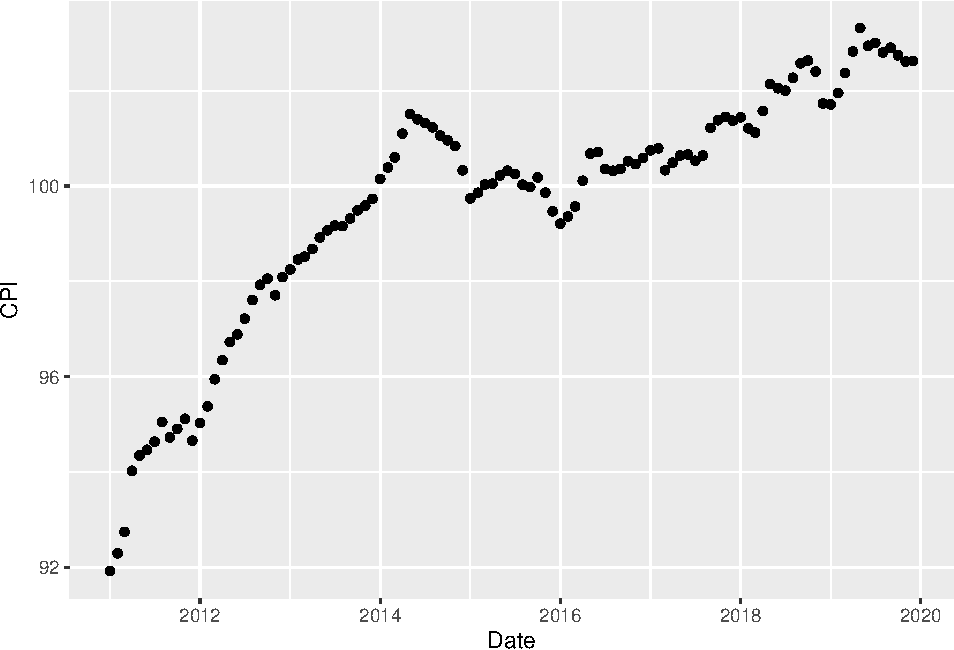
\includegraphics{figCPI-1} 

}

\caption{The monthly consumer price indices from January 2011 to December 2019}\label{fig:figCPI}
\end{figure}

\begin{figure}
\centering
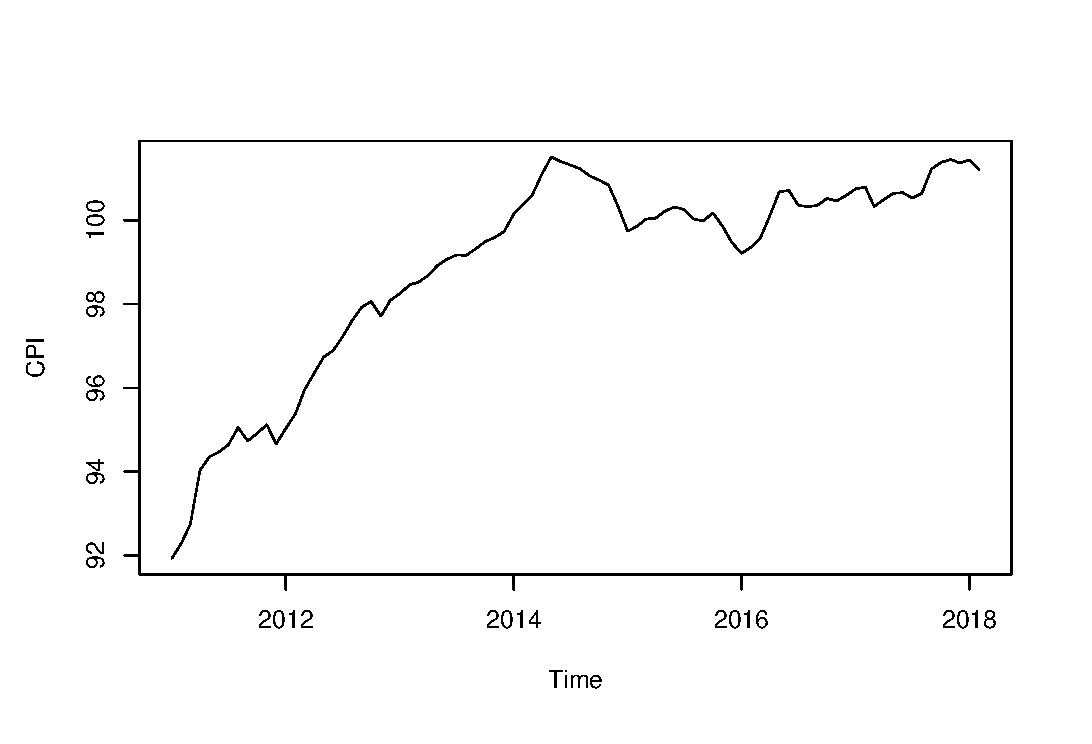
\includegraphics{CPIGraph.eps}
\caption{image}
\end{figure}

\newpage \begin{example}
\protect\hypertarget{exm:unlabeled-div-53}{}\label{exm:unlabeled-div-53}

\emph{An investment contract made on January 2018 promises
to pay an investor of ฿10,000 in 5 years' time. Assume the average
inflation rate at \(\bar{q} = 0.64\%\) for the next 5 years.}

\emph{If a bowl of noodles costs ฿100 in 2018, then ฿10,000 could buy 100
bowls. How many bowls of noodles would the payment of ฿10,000 buy in the
next 5 years?}

\emph{\textbf{Solution:} In Jan 2018, ฿100 buys as much as \(100 (1.0064)^5 =\)
฿103.2 in Jan 2023.}

\emph{So ฿10000 in Jan 2023 could buy
\[\frac{10000}{103.2} \approx 96 \text{ bowls}.\] Notice that we divide
by \((1 + \bar{q})^5\) to calculate how much your money is worth at the
end of the next five years.}

\begin{itemize}
\item
  \emph{The quantity of goods that can be bought with 10,000 in January
  2023 reduces from 100 to 96 bowls.}
\item
  \emph{The effect of inflation results in the reduction of the purchasing
  power of a unit of money in January 2023 compared to that in
  January 2018.}
\item
  \emph{The amount of ฿10,000 is referred to as the \textbf{monetary} (or
  \textbf{nominal}) payment in 5 years. This is the amount of money that
  change hands.}
\item
  \emph{The \textbf{real payment of ฿10,000 (due at time 5 years) in time 0
  unit} is \[\begin{aligned}
  10000 \frac{Q(0)}{Q(5)} &=  10000  \frac{1}{(1.0064)^5} \\
                           &=  9686.05.\end{aligned}\] Here we have
  less purchasing power with your money at the end of the five years
  than you had at the start of the year.}
\item
  \emph{The real payment (in time 0) is the purchase power of 10,000 paid
  in 5 years relative to today. \textbf{It is the amount of cash in hand at
  the end of the period reduced for the effects of inflation}.}
\item
  \emph{In general, ฿X at time \(t\) has the purchasing power relative to
  time \(s\) of \[X \cdot \frac{Q(s)}{Q(t)}.\]}
\end{itemize}

\end{example}

\hypertarget{real-rates-of-interest}{%
\subsection{Real rates of interest}\label{real-rates-of-interest}}

The rate of interest which is calculated using monetary payments is
called a \textbf{money (or monetary or nominal) rate of interest}.

The \textbf{real rate of interest} is calculated using real payments.

\newpage \begin{example}
\protect\hypertarget{exm:unlabeled-div-54}{}\label{exm:unlabeled-div-54}

\emph{An investor deposits 100 at time 0 and receives 120
after one year.}

\begin{itemize}
\item
  \emph{The monetary rate of interest effective is
  \[\frac{120}{100} - 1 = 20\%.\]}
\item
  \emph{Suppose that the inflation rate over this one year period is 4\%.
  Calculate the real payment of 120 at time 1 and the real rate of
  interest. After adjusting for the inflation rate, the real rate of
  interest can be calculated by first expressing both payments in
  units of the same purchasing power.}

  \begin{itemize}
  \item
    \emph{In term of time 0 money unit, the transaction is represented
    by}

    \emph{Here, the real payment of 120 due in 1 year in terms of time 0
    unit is \(\displaystyle{120 \cdot \frac{1}{1.04} = 115.38}\).
    Hence the real rate of interest is 15.38\%.}
  \item
    \emph{In term of time 1 money unit, the transaction is represented
    by}

    \emph{Similarly, we instead calculate the real payment of 100
    relative to time 1, which gives \(100 \cdot 1.04 = 104\). The real
    rate of interest is \[\frac{120}{104} - 1 = 15.38\%,\] which is
    the same as the previous case.}
  \end{itemize}
\end{itemize}

\end{example}

\hypertarget{real-yields}{%
\subsection{Real yields}\label{real-yields}}

It is often useful to look at the rate of return earned on an investment
after taking into account of inflation. As analogous to the real rate of
interest, a \textbf{real yield} is calculated using real payments, which can
be obtained by expressing payments in units of the same purchasing power
\textbf{at some specific date}.

\newpage \begin{example}
\protect\hypertarget{exm:unlabeled-div-55}{}\label{exm:unlabeled-div-55}

\emph{A 5-year bond with nominal value of ฿100 was issued
in January 2013. The coupon rate was 8\% p.a. payable yearly in arrears.
Redemption was at par after 5 years. The bond was issued at 100\%.
Calculate the yield to a non-tax paying investor}

\begin{enumerate}
\def\labelenumi{\arabic{enumi}.}
\item
  \emph{in monetary terms \textbf{Solution:}}

  \emph{The transaction together with the inflation indices \(Q(t)\) at time
  \(t\) is shown as follows:}

  \emph{Clearly, the monetary rate of return on this transaction is 8\%.
  This is because the investor receives the interest payment of ฿8 at
  the end of each year plus the initial capital of ฿100 at the end of
  five years.}

  \emph{Alternatively, one can solve for the monetary rate of return from
  the following equation of value
  \[f(i) = -100 + 8 a^i_{\actuarialangle{5}} + 100\frac{1}{(1+i)^5} = 0.\]}
\item
  \emph{in real terms with reference to the CPI.}

  \emph{Taking into account of the inflation rates, we calculate the real
  payment in term of time 0 unit by dividing the monetary amounts by
  the \textbf{proportional} increase in the inflation index from 0 to \(t\).}

  \emph{The real yield \(i'\) p.a. effective solve the equation of value as
  follows:
  \[f(i') = -100 + 7.85 v  + 7.88v^2 + 7.91v^3 + 7.80v^6 + 104.6v^5 = 0,\]
  which gives \(i' \approx 7.30\%\) by the linear interpolation.}
\end{enumerate}

\end{example}

In general, the real yield \(i'\) for a series of cashflows
\(C(t_1), C(t_2), \ldots, C(t_n)\), given associated inflation index
\(Q(t_k)\) for \(k = 1, \ldots, n\), can be obtained in terms of time 0
money units as
\[\sum_{k=1}^n C(t_k) \frac{Q(0)}{Q(t_k)} \frac{1}{(1 + i')^{t_k}} = 0.\]
This is equivalent to
\[\sum_{k=1}^n C(t_k) \frac{1}{Q(t_k)} \frac{1}{(1 + i')^{t_k}} = 0.\]
Therefore, \textbf{the real yield is independent of the date the payment units
are adjusted to}.

\hypertarget{calculating-real-yields-given-constant-inflation-assumptions}{%
\subsection{Calculating real yields given constant inflation assumptions}\label{calculating-real-yields-given-constant-inflation-assumptions}}

For future cashflows, the inflation index will not be known. Suppose we
assume a constant rate of inflation \(q\) p.a. The cashflows \(C(t_k)\) at
time \(t_k\) have the purchasing power at time 0 (or real payments
relative to time 0) \[\begin{aligned}
    C(t_k) \cdot \frac{Q(0)}{Q(t_k)} &=     C(t_k) \cdot \frac{Q(0)}{Q(0)(1+q)^{t_k}}  =  C(t_k) \cdot \frac{1}{(1+q)^{t_k}} , \quad k = 1, \ldots, n.\end{aligned}\]
The relation between the real yield \(i'\), the constant rate of inflation
\(q\) and the monetary yield \(i\) can be obtained as follows: From the
equation of value, \[\begin{aligned}
    0   &= \sum_{k=1}^n C(t_k) \frac{Q(0)}{Q(t_k)} \frac{1}{(1 + i')^{t_k}} \\
        &=  \sum_{k=1}^n C(t_k)  \cdot \frac{1}{(1+q)^{t_k}}\cdot \frac{1}{(1 + i')^{t_k}}\end{aligned}\]
With no inflation adjustment, the monetary rate of return \(i\) satisfies
\[0 =  \sum_{k=1}^n C(t_k)  \cdot \frac{1}{(1+i)^{t_k}}.\] Therefore, if
\textbf{we assume a constant rate of inflation} \(q\) p.a., then the following
relation holds: \[(1 +i) = ( 1 + q)(1+i').\] This provides the
relationship between the real yield \(i'\), the monetary yield \(i\) and the
inflation rate \(q\).

\hypertarget{index-linked-securities}{%
\subsection{Index-linked securities}\label{index-linked-securities}}

An index-linked security is an investment security in which interest
payments and the redemption are adjusted in line with inflation index
values by linking the payments to the Consumer Price Index (CPI). The
reasons for these types of security are

\begin{itemize}
\item
  to protect investors against inflation risk, and
\item
  to help pension funds to provide index-link benefits so that the
  index-link liability can be matched with the index-link asset.
\end{itemize}

\newpage \begin{example}
\protect\hypertarget{exm:unlabeled-div-56}{}\label{exm:unlabeled-div-56}

\emph{Consider an index-link bond of a nominal of ฿100
issued at time \(t_0\), bearing an annual coupon of \(C\%\) payable \(m\)
times a year and a redemption is at \(R\%\). Then per ฿100 nominal, the
monetary amount (actual cashflow) of an interest payment \(D(t_k)\) at
time \(t_k\) is}

\emph{The monetary amount of the redemption amount at time \(t_n\) is}

\end{example}

\newpage \begin{example}
\protect\hypertarget{exm:exampleILB}{}\label{exm:exampleILB}

\emph{An investor purchased a 3-year index-linked bond in
January 2015. The investor received payments at the end of each year
plus a final redemption amount, all of which were adjusted in line with
the CPI values reported in Table \ref{tab:tableCPI}.
Calculate the actual payments received by the investor.}

\end{example}

\textbf{Note} In practice, due to delays in calculating the index, the
payments (or cashflows) will be adjusted based on the inflation index
value from an earlier period.

Let \(s\) denote the indexation time lag. The payments are adjusted with
reference to inflation index value at time \(s\) (months) before the
payment is made. Then the monetary amount of an interest payment
\(D(t_k)\) per ฿100 nominal at time \(t_k\) is
\[\displaystyle D(t_k) = 100 \frac{C}{m} \cdot \frac{Q(t_k - \frac{s}{12})}{Q(t_0 - \frac{s}{12})}\]
and the monetary amount of redemption at time \(t_n\) is
\[D(t_n) = 100 R \cdot \frac{Q(t_n - \frac{s}{12})}{Q(t_0 - \frac{s}{12})}.\]
The term \(Q(t_0 - \frac{s}{12})\) is called the base inflation figure
(the base CPI figure).

\newpage \begin{example}
\protect\hypertarget{exm:unlabeled-div-57}{}\label{exm:unlabeled-div-57}

\emph{Repeat Example\ref{exm:exampleILB}
for a 3-year index linked bond. The indexation adjustments are made
according to the CPI three months before each payment, i.e.~\(s = 3\)
months.}

\end{example}

\newpage \begin{example}
\protect\hypertarget{exm:exampleILB2}{}\label{exm:exampleILB2}

\emph{In January 2015, the government issued an
index-linked bond of term 10 years. Coupons are payable half-yearly in
arrears, and the annual nominal coupon rate is 4\%. The coupons and
redemption amount are adjusted with reference to the inflation index
value 3 months before the payment is made.}

\emph{Assume the constant inflation rate from February 2018 is 2\% p.a.}

\begin{enumerate}
\def\labelenumi{\arabic{enumi}.}
\item
  \emph{Find the base CPI figure (i.e.~it is the October 2014 CPI which is
  3 months before the issue date).}
\item
  \emph{Calculate the actual payments received by the investor.}
\item
  \emph{Assume that the price of ฿100 nominal of this index-linked bond in
  January 2018 (after the January 2018 coupon payment) is ฿ .
  Calculate the monetary yield that an investor who purchased the bond
  in January 2018 (after the January 2018 coupon payment) will
  obtained.}
\item
  \emph{Calculate the real yield for this investor under the above
  assumptions.}
\end{enumerate}

\end{example}

\hypertarget{processes-for-stock-prices}{%
\chapter{Processes for stock prices}\label{processes-for-stock-prices}}

In this chapter, we will consider some models (or processes) that are
used to model stock price. The prices of stocks are continuous in time
and value, which are unpredictable. However, we assume that stock prices
follow a type of models (which are stochastic processes) known as
\textbf{geometric Brownian motion}. This is one of the main tools in
mathematical financial used in an analysis of derivatives. You will
study in more details in the course ``SCMA 459 Investment Science II''.

We will first begin with the brief introduction of the \textbf{force of
interest} (or \textbf{continuous compounding}). The process for a stock
price and an algorithm to simulate stock prices will be presented after
main concepts of random walks and Brownian motion are given.

\hypertarget{force-of-interest}{%
\section{Force of interest}\label{force-of-interest}}

Given an annual effective rate \(i\), a principal of 1 accumulates to
\((1 + i)\) at the end of the first year. The following formula provides
the \textbf{equivalent nominal rates}, \(i^{(n)}\), of interest convertible \(n\)
times per year, \[\left(1 + \frac{i^{(n)}}{n} \right)^n  = (1 + i),\]
which gives \[i^{(n)} = n\left( (1+ i)^{1/n} - 1  \right).\] Note that
\(\displaystyle{\frac{i^{(n)}}{n}}\) is the effect interest rate applied
for each \(n\)-th of a year. For e.g.~if \(n =2\), then
\(\displaystyle{\frac{i^{(2)}}{2}}\) is the half-yearly effect interest
rate equivalent to \(i\).

\newpage \begin{example}
\protect\hypertarget{exm:unlabeled-div-58}{}\label{exm:unlabeled-div-58}

\emph{Given the annual effective rate \(i = 4\%\),}

\begin{enumerate}
\def\labelenumi{\arabic{enumi}.}
\item
  \emph{calculate the equivalent nominal rates of interest convertible \(n\)
  times a year for \(n = 2,4,12, 52,\) and 365,}
\item
  \emph{find the limit of \(i^{(n)}\) as \(n\) tends to infinity, and}
\item
  \emph{plot the graph of \(i^{(n)}\) as a function of \(n\).}
\end{enumerate}

\end{example}

\textbf{Notes}

\begin{enumerate}
\def\labelenumi{\arabic{enumi}.}
\item
  Using the result from calculus, we can show that
  \[\lim_{n \rightarrow \infty} \left(1 + \frac{x}{n} \right)^n = \exp(x).\]
\item
  As \(n\) tends to infinity, a rate of \(i^{(n)}\) compounding \(n\) times
  a year converges to a constant, which will be denoted by \(\delta\),
  i.e.~\(i^{(n)} \rightarrow \delta\) as \(n \rightarrow \infty\).
\item
  The above observations imply following relation:
  \[\lim_{n \rightarrow \infty} \left(1 + \frac{i^{(n)}}{n} \right)^n  = \exp(i^{(\infty)}) = \exp(\delta),\]
  where we write \(i^{(\infty)} = \delta\).
\item
  The constant \(\delta\) is known as the \textbf{force of interest} or also
  known as a \textbf{continuous compounded rate}. It is the interest rate
  paid continuously throughout the period. It is a constant \textbf{force}
  that causes the initial investment to grow.
\item
  The following relationship between the force of interest and the
  annual effective rate of interest holds:
  \[1 + i = \exp(\delta) \quad \text { or } \delta = \ln(1+i).\]
\end{enumerate}

\newpage \begin{example}
\protect\hypertarget{exm:unlabeled-div-59}{}\label{exm:unlabeled-div-59}

\emph{฿200 is invested in an account which pays a force of
interest of 4\% pa. Calculate the amount in the account after 3 years.}

\end{example}

\newpage \begin{example}
\protect\hypertarget{exm:unlabeled-div-60}{}\label{exm:unlabeled-div-60}

\emph{A payment of ฿500 is due in 5 years' time. Calculate
the present value of this payment at a force of interest of 4\% pa.}

\end{example}

For a force of interest \(\delta\), the accumulation at time \(t\) of 1 unit
paid at time \(s\) is \[A(s,t) = \exp( \delta (t-s)).\] The present value
at time \(s\) of 1 unit paid at time \(t\) is
\[V(s,t) = \exp( -\delta (t-s)).\] \textbf{Notes}

\begin{enumerate}
\def\labelenumi{\arabic{enumi}.}
\item
  In general, the force of interest \(\delta(t)\) per annum at time \(t\)
  is a function of \(t\).
\item
  Given the force of interest per annum \(\delta(t)\), the accumulation
  at time \(t\) of 1 unit paid at time \(s\) is
  \[A(s,t) = \exp\left( \int_{s}^t \delta(s) \, ds  \right).\]

  Also, the present value at time \(s\) of 1 unit paid at time \(t\) is
  \[V(s,t) = \exp\left(- \int_{s}^t \delta(s) \, ds  \right).\]
\item
  The more detailed discussion regarding the force of interest and
  continuous cashflows will be given in the course SCMA 361 Theory of
  Interest.
\end{enumerate}

The diagram below shows the accumulation at time \(t\) of 1 unit paid at
time \(s\) at the annual effective rate \(i\) and the force of interest
\(\delta(t)\).

\newpage \begin{example}
\protect\hypertarget{exm:unlabeled-div-61}{}\label{exm:unlabeled-div-61}

\emph{A payment of ฿1000 is due in 1 years' time. Calculate
the accumulated amount at time 1 of this payment at a force of interest
of \(\delta(t)\) pa, where \[\delta(t) = a + b t + c t^2,\] \(a,b\) and \(c\)
are given constants.}

\end{example}

\hypertarget{stochastic-processes}{%
\section{Stochastic processes}\label{stochastic-processes}}

It is of great interest to model the behaviour of a system by describing
how different states, describe by random variables \(X\)'s, in the system
evolve with time.

Stochastic processes can be used to represent many different phenomena
from various areas including science, engineering, finance, and
economics. As opposed to a deterministic model whose outcome is fixed,
the outcome of a stochastic process is not certain, the stochastic
process is simply a collection of random variables defined as follows:

A \textbf{stochastic process} is a collection of random variables
\(\{ X_t : t \in T\}\), where

\begin{itemize}
\item
  \(t\) is a parameter running over some index set \(T\), called the
  \textbf{time domain}.
\item
  The common sample space of the random variables (the range of
  possible values for \(X_t\)) denoted by \(S\) is called the \textbf{state
  space} of the process.
\end{itemize}

\textbf{Notes}

\begin{enumerate}
\def\labelenumi{\arabic{enumi}.}
\item
  The set of random variables may be dependent or need not be
  identically distributed.
\item
  Techniques used to study stochastic processes depend on whether the
  state space or the index set (the time domain) are discrete or
  continuous.
\item
  Topics on stochastic processes will be discussed in the course ``SCMA
  469 Actuarial Statistics''.
\end{enumerate}

\hypertarget{a-simple-random-walk}{%
\subsection{A simple random walk}\label{a-simple-random-walk}}

Consider a simple model of the price of a stock measured in units of
Thai baht. For each trading day \(n = 0,1,2, \ldots\), the stock price
increases by 1 baht with probability \(p\) or decreases by 1 baht with
probability \(q = 1-p\).

Let \(X_n\) denote the stock price at day \(n\) and \(X_0 =\) ฿100. This
simple model is called a \textbf{simple random walk}.

In general, a simple random walk \(X_n\) is a discrete-time stochastic
process defined by

\begin{itemize}
\item
  \(X_0 = a\) and
\item
  for \(n \ge1\),
  \[X_n = a + \sum_{i=1}^n  Z_i, \text{ where } Z_i = \begin{cases}
      1, & \text{ with probability } p  \\
      -1, & \text{ with probability } q =  1- p.
   \end{cases}\]
\end{itemize}

\textbf{Note} When \(p = 1/2\), the value of the process increases or decreases
randomly by 1 unit with equal probability. In this case, the process is
known as a \textbf{symmetric} random walk.

\newpage \begin{example}
\protect\hypertarget{exm:unlabeled-div-62}{}\label{exm:unlabeled-div-62}

\emph{Calculate the expectation and variance of the random
variable \(Z_i\).}

\end{example}

\textbf{Solution:} \[\begin{aligned}
    \mu &= \mathrm{E}[Z_i] = 1\cdot p + (-1) \cdot q = p - q.\\\end{aligned}\]
\[\begin{aligned}
    \sigma^2 &= \mathrm{Var}[Z_i] \\
            &=\mathrm{E}[Z_i^2] - (\mathrm{E}[Z_i] )^2 \\
            &= 1 - (p-q)^2  = (p+q)^2 - (p-q)^2\\
            &= 4pq.\end{aligned}\]

\newpage \begin{example}
\protect\hypertarget{exm:unlabeled-div-63}{}\label{exm:unlabeled-div-63}

\emph{Calculate the expectation and variance of the process
\(X_n\) at time \(n\).}

\end{example}

\textbf{Solution:} \[\begin{aligned}
     \mathrm{E}[X_n] &=  \mathrm{E}[a + \sum_{i=1}^n Z_i] = a + n\mu.\end{aligned}\]
\[\begin{aligned}
    \mathrm{Var}[X_n]&= \mathrm{Var}[a + \sum_{i=1}^n Z_i]  = n \sigma^2.\end{aligned}\]
It should be noted that the variance of \(X_n\) increases with time.

The next example shows how to use a coin to simulate price paths of a
stock.

\newpage \begin{example}
\protect\hypertarget{exm:unlabeled-div-64}{}\label{exm:unlabeled-div-64}

\emph{We flip the coin once to represent each trading day.
If the coin comes up head then the stock price goes up by 1 baht; if it
comes up tail then the stock price goes down by 1 baht. Assume that the
initial stock price is \(X_0 = 100\). Let us flip the coin 20 times and
then draw the graph of the stock price against time (in day). Repeat
this process 4 more times.}

\end{example}

\textbf{Solution:} See the Excel worksheet.

\hypertarget{sample-paths}{%
\subsection{Sample paths}\label{sample-paths}}

In the simple random walk process, time is discrete (as observed at the
end of each day) and the state space is discrete. The stochastic model
has an infinite number of \textbf{stochastic realisations}. A \textbf{sample path}
is then just the sequence of a particular set of experiments. Graphs of
some stochastic realisations of the simple random walk with \(p = 0.5\)
and \(a = 100\) are shown in Figure are shown in Figure \ref{fig:FigRW}.

\begin{figure}
\centering
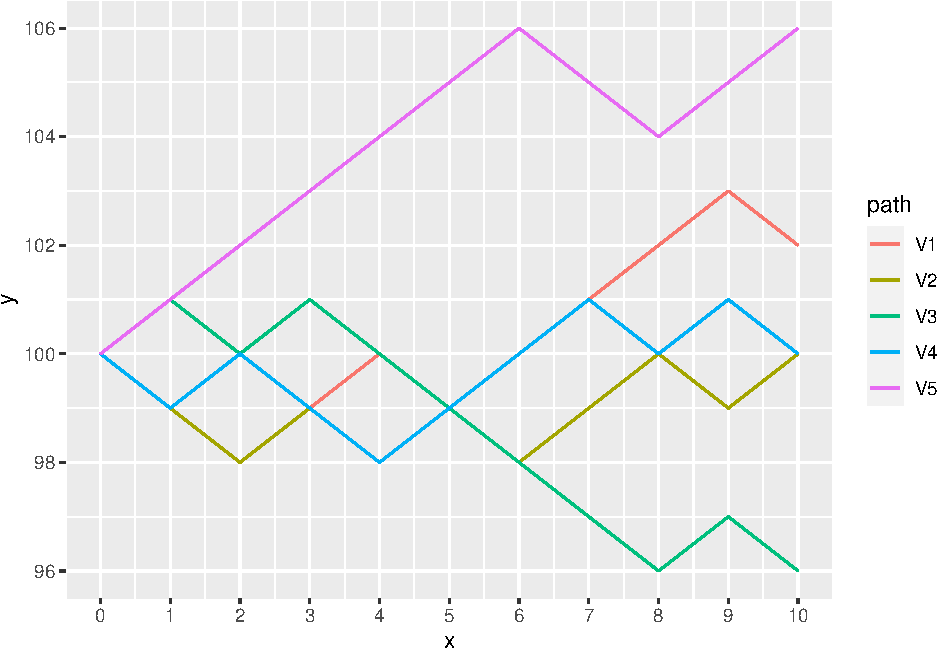
\includegraphics{FigRW-1.pdf}
\caption{\label{fig:FigRW}Some stochastic realisations of the simple random walk}
\end{figure}

\newpage \begin{example}
\protect\hypertarget{exm:unlabeled-div-65}{}\label{exm:unlabeled-div-65}

\emph{For the random process, calculate
\[\Pr(X_2 = 98, X_5 = 99 | X_0 = 100).\]}

\end{example}

\textbf{Solution:} The process \(X_n\) must decrease on the first two days,
which happens with probability \((1-p)^2\). Independently, it must then
increases on another two days and decrease on one day (not necessarily
in that order), giving three different possibilities. Each of these has
probability \(p^2(1-p)\). So
\[\Pr(X_2 = 98, X_5 = 99 | X_0 = 100) = (1-p)^2 \cdot 3 p^2(1-p) = 3p^2(1-p)^3.\]

\begin{figure}
\hypertarget{fig:SamplePaths}{%
\centering
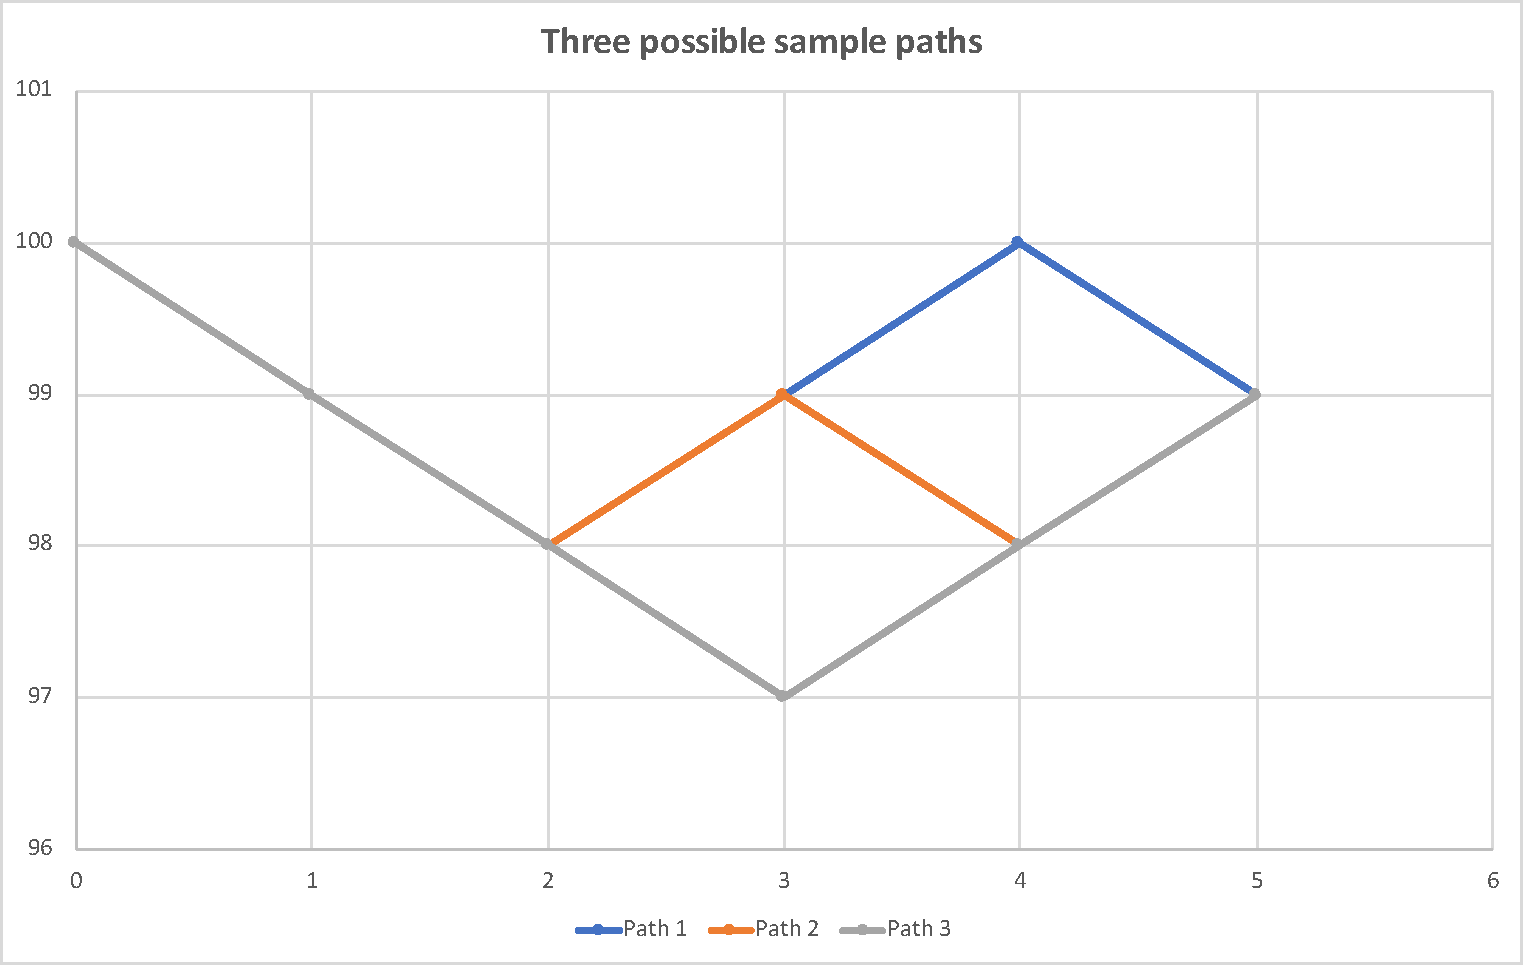
\includegraphics[width=3in,height=\textheight]{RWThreePaths.pdf}
\caption{Three possible sample paths}\label{fig:SamplePaths}
}
\end{figure}

\hypertarget{simulating-a-simple-random-walk}{%
\subsection{Simulating a simple random walk}\label{simulating-a-simple-random-walk}}

To simulate a sample path of the simple random walk process \(X_n\) for
\(n = 0,1, \ldots, N\), we proceed as follows:

\begin{enumerate}
\def\labelenumi{\arabic{enumi}.}
\item
  Generate \(N\) random samples from the discrete distribution of the
  random variable \(Z_i\), \(i = 1,\ldots, N\), as follows:

  \begin{enumerate}
  \def\labelenumii{\arabic{enumii}.}
  \item
    We first generate random numbers from the uniform distribution
    \(U(0,1)\). Denote these numbers by \(U_i\).
  \item
    If \(U_i \le p\), then set \(Z_i = 1\). Otherwise, \(Z_i = -1\)
  \end{enumerate}
\item
  The value \(X_n\) of the random walk process at time \(n\),
  \(1 \le n \le N\), can then be calculated from
  \[X_n = a + \sum_{i=1}^n  Z_i.\]
\end{enumerate}

\textbf{Notes}

\begin{enumerate}
\def\labelenumi{\arabic{enumi}.}
\item
  Excel provides two function \textbf{RAND()} and \textbf{RANDBETWEEN(a,b)} to
  generate a random number between 0 and 1 and a random integer
  between \(a\) and \(b\).
\item
  Excel also provides Random Number Generation to draw sample numbers
  from some specified distributions (to be discussed in Excel Lab).
\end{enumerate}

\begin{figure}
\hypertarget{fig:RW}{%
\centering
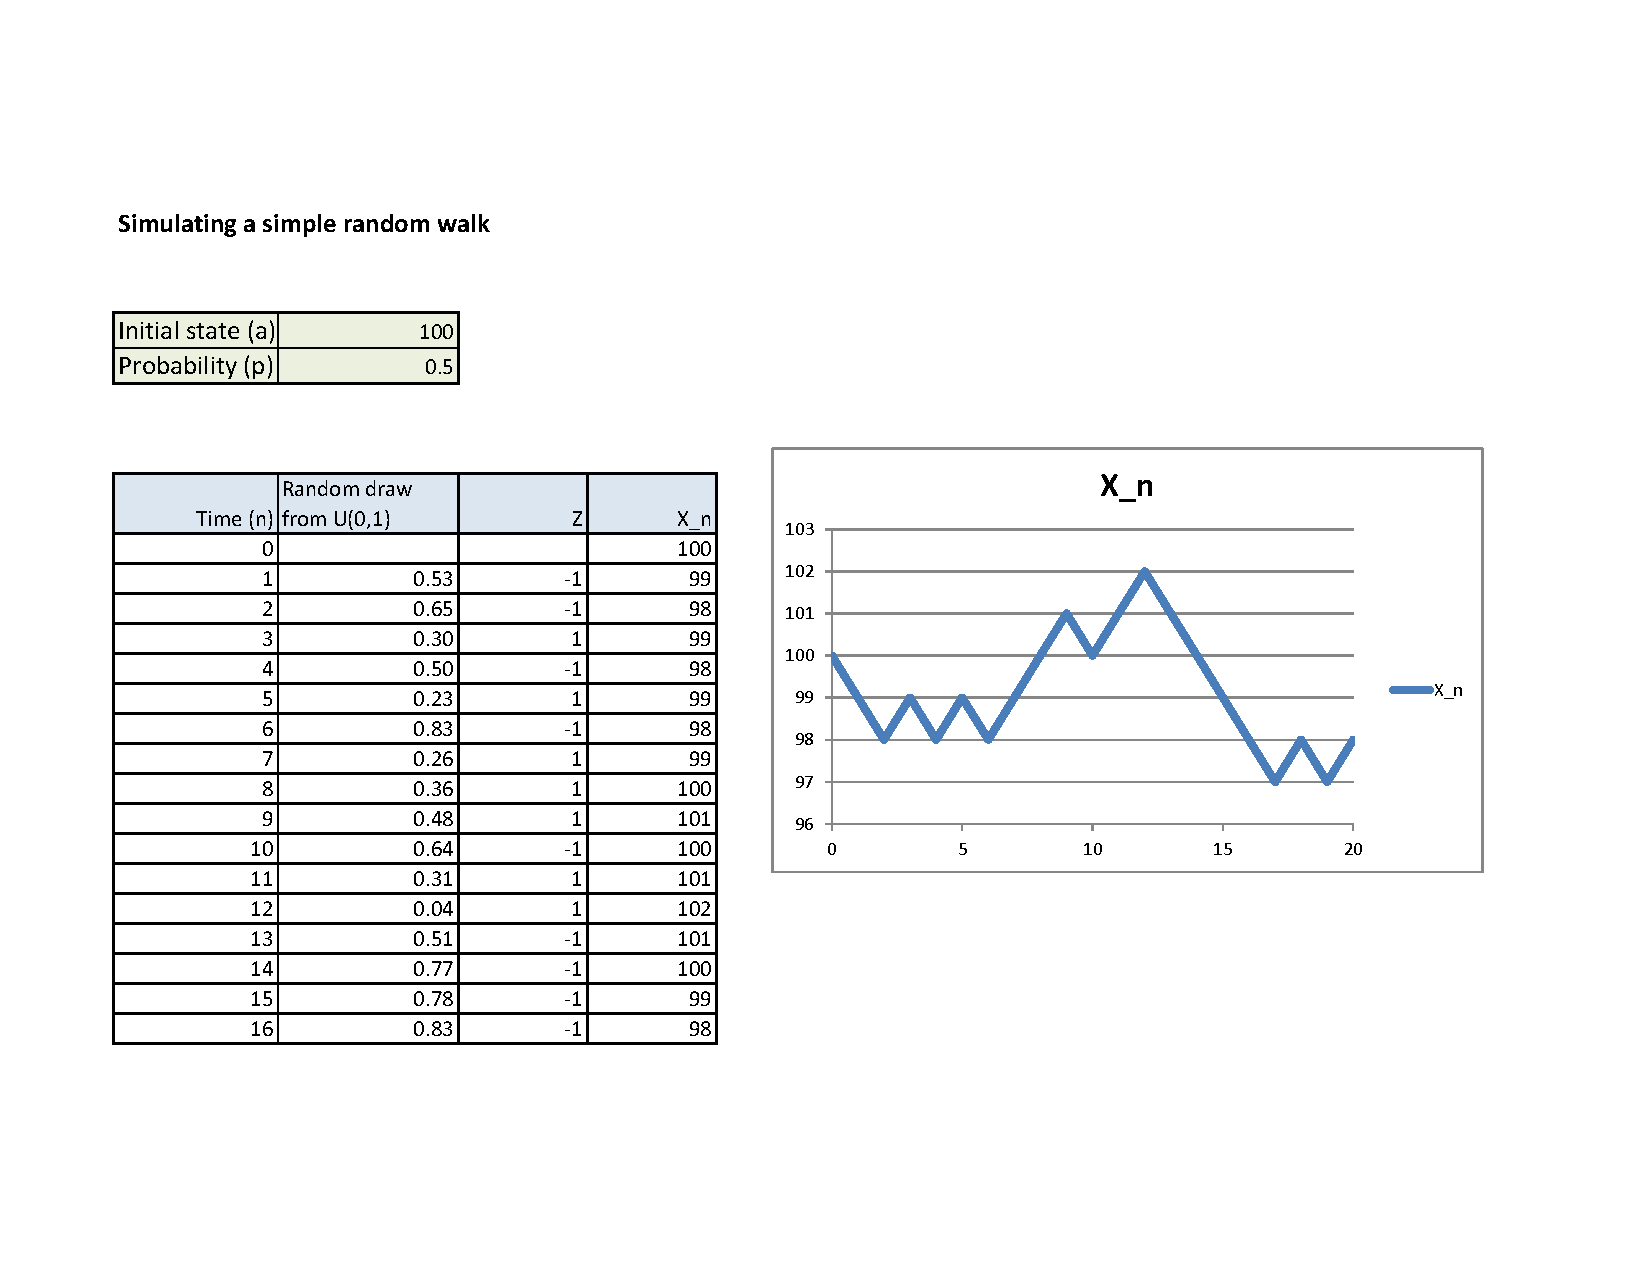
\includegraphics[width=8in,height=\textheight]{RW.pdf}
\caption{Simulating a sample path of a simple random walk}\label{fig:RW}
}
\end{figure}

\hypertarget{monte-carlo-methods}{%
\section{Monte Carlo Methods}\label{monte-carlo-methods}}

Monte Carlo methods are simulation-based algorithms that rely on
generating a large set of samples from a statistical model to obtain the
behaviour of the model and estimate the quantities of interest. For a
large sample set of a random variable representing a quantity of
interest, the law of large numbers allows to approximate the expectation
by the average value from the samples.

Consider repeated independent trials of a random experiment. We will
need to generate a large number of samples \(X_1, X_2, \ldots\) from the
model. A Monte Carlo method for estimating the expectation
\(\mathrm{E}[ X ]\) is a numerical method based on the approximation
\[\mathrm{E}[ X] \approx \frac{1}{N}\sum_{i=1}^N X_i,\] where
\(X_1, X_2, \ldots\) are i.i.d. with the same distribution as \(X\).

While computing expectations and computing probabilities at first look
like different problems, the latter can be reduced to the former: if \(X\)
is a random variable, we have
\[\Pr(X \in A) = \mathrm{E}[\mathbbm{1}_A(X)].\]

Using this equality, we can estimate \(\Pr(X \in A)\) by
\[\Pr(X \in A) = \mathrm{E}[\mathbbm{1}_A(X)] = \frac{1}{N}\sum_{i=1}^N \mathbbm{1}_A(X_i).\]

Recall that the indicator function of the set \(A\) is the defined as
\[\mathbbm{1}_A(x) =
\begin{cases*}
     1          & if $x \in A $ \\
      0        & otherwise.
\end{cases*}\]

\newpage \begin{example}
\protect\hypertarget{exm:unlabeled-div-66}{}\label{exm:unlabeled-div-66}

\emph{Using Monte Carlo estimation, approximate the
expectation \(\mathrm{E}[X]\) where \(X \sim \mathcal{N}(0,1)\), and
estimate the percent of values lie within two standard deviation of the
mean of \(X\)}

\end{example}

\textbf{Solution:} We generate samples \(X_1,X_2,...,X_N\) from the model \(X\)
for large \(N\), for example for \(N = 10000\), we can use estimates such as
\[\mathrm{E}[X] \approx \frac{1}{N}\sum_{i=1}^N X_i,\] and
\[\mathrm{Var}[X] \approx \frac{1}{N-1}\sum_{i=1}^N (X_i - \bar{X})^2.\]

\hypertarget{the-markov-property}{%
\section{The Markov Property}\label{the-markov-property}}

A Markov process is a special type of stochastic processes with the
property that the future evolution of the process depends only on its
current state and not on its past history.

That is given the value of \(X_t\), the values of \(X_s\) for \(s > t\) do not
depend on the values of \(X_u\) for \(u < t\). This property is called the
\textbf{Markov property}.

A \textbf{Markov process} is any stochastic process that satisfies the Markov
property

\textbf{Notes}

\begin{enumerate}
\def\labelenumi{\arabic{enumi}.}
\item
  Stock prices are usually assumed to follow a Markov process where
  only the current stock price is relevant for predicting future
  prices, and thus the past values are irrelevant
\item
  Predictions in the future is uncertain, and must be expressed in
  terms of probability distributions. Hence, the probability
  distribution of the future stock price is independent of the
  particular price path in the past.
\item
  \textbf{Time series models} are widely used in economics, business and
  engineering to predict the variability of a variable over time,
  where past values are used as the input variables for the model.
\end{enumerate}

\hypertarget{wiener-processes}{%
\section{Wiener processes}\label{wiener-processes}}

We start with the Markov process that is a building block for the
geometric Brownian motion. Analogously to the random walk process, it is
defined in terms of some simple intermediary processes, that is the
increment process \(Z_i\). The \textbf{Wiener process} is a Markov process
which will be used to \textbf{model the change in the stock prices}.

The Wiener process is a (\textbf{continuous-time stochastic}) process which
can be described by a variable \(W\) having the following properties:

\begin{itemize}
\item
  We assume that the current value is 0 (i.e.~\(W(0) = 0\)) and \textbf{the
  change in its value during a year} (i.e.~\(W(1) - W(0)\)) is \(N(0,1)\)
  where \(N(m,v)\) is a probability distribution normally distributed
  with mean \(m\) and variance \(v\).

  \textbf{Notes} The following properties of the normal distributions are
  useful.

  \begin{enumerate}
  \def\labelenumi{\arabic{enumi}.}
  \item
    Given \(X \sim N(\mu, \sigma^2), Y = a + bX\), it follows that
    \[Y \sim N(a + b\cdot \mu, b^2 \sigma^2).\]
  \item
    Given \(X \sim N(\mu_X, \sigma_X^2), Y \sim N(\mu_Y, \sigma_Y^2)\)
    with \(X, Y\) independent, it follows that
    \[X + Y  \sim N(\mu_X + \mu_Y, \sigma_X^2 + \sigma_Y^2).\]
  \item
    It is well known that if two i.i.d. random variables are
    normally distributed, their sum is also normally distributed.

    The converse is also true.

    That is, suppose \(X\) and \(Y\) are two i.i.d. random variables
    such that \(X + Y\) is normal. It necessarily the case that \(X\)
    and \(Y\) are also normal.
  \end{enumerate}
\item
  The probability distribution of the change in the value of the
  variable during any time period of length \(T\) is \(N(0,T)\). For
  example,

  \begin{itemize}
  \item
    The change in 2 years is the sum of two normal distributions,
    each of which has mean of 0 and variance of 1. \textbf{Solution:}
    \[\begin{aligned}
        W(2) - W(0) &= (W(2) - W(1)) +  (W(1) - W(0)) \\
                  &\sim X + Y \text{ where } X, Y \text{ are independent } N(0,1)                   \text{ distributions.}  \\
                  &\sim N(0,2).\end{aligned}\]

    The Markov property implies that the two distributions are
    \textbf{independent}. Hence the sum of two independent normal
    distributions is a normal distribution where the mean is the sum
    of the means and the variance is the sum of the variances.

    The the probability distribution of the change in the value of
    the variable in 2 years is \(N(0,2)\).
  \item
    For the change in 6 months, the variance of the change in the
    value of the variable during 1 year (which is 1) equals to the
    sum of the variance of the change in the first 6 months and the
    second 6 months. We also assume that the two distributions of
    the six-months period are the same (or \textbf{identical}). As a
    result, the the probability distribution of the change in the
    value of the variable during 6 months is \(N(0,0.5)\).

    \textbf{Solution:} \[\begin{aligned}
        W(1) - W(0) &= (W(1) - W(0.5)) +  (W(0.5) - W(0)) \\
                  &\sim U + V \text{ where } U, V \text{ are identical and independent}\end{aligned}\]
    Since \(W(1) - W(0) \sim N(0,1)\), it follows that \(U\) and \(V\) are
    both normally distributed \(N(0,0.5)\).
  \end{itemize}
\end{itemize}

\newpage \begin{example}
\protect\hypertarget{exm:unlabeled-div-67}{}\label{exm:unlabeled-div-67}

\emph{Given that \(W(0) = a\), what is the probability
distribution of the value of W at 3 months, i.e.~\(W(0.25)\)?}

\end{example}

\textbf{Solution:} \[\begin{aligned}
    W(0.25) &= W(0) + (W(0.25) - W(0)) \\
            & \sim a + N(0,0.25)  \\
            & \sim N(a, 0.25).\end{aligned}\] The mean and the variance
of \(W(0.25)\) is \(a\) and 0.25, respectively.

More precisely, a \textbf{standard Brownian motion} or \textbf{standard Wiener
process} over \([0,T]\) is a random variable \(W(t)\) that depends
continuously on \(t \in [0,T]\) and satisfies the following conditions:

\begin{enumerate}
\def\labelenumi{\arabic{enumi}.}
\item
  \(W(0) = 0\) (with probability 1).
\item
  For \(0 \le s < t \le T\), the \textbf{change (or increment)} \(W(t) - W(s)\)
  is normally distributed with mean zero and variance \(t -s\).
\item
  For \(0 \le s < t < u < v \le T\), the change (or increment)
  \(W(t) - W(s)\) and \(W(v) - W(u)\) are independent.
\end{enumerate}

\textbf{Notes}

\begin{enumerate}
\def\labelenumi{\arabic{enumi}.}
\item
  The second condition above implies that the change
  \(W(t) - W(s) \sim \sqrt{t-s} N(0,1)\), where \(N(0,1)\) denotes a
  normally distributed random variable with mean zero and unit
  variance.
\item
  The uncertainty about the value of the standard Brownian motion
  measured in terms of its standard deviation increases as the square
  root of how far we are looking ahead, i.e.~the square root of the
  length of the period considered.
\end{enumerate}

\hypertarget{simulating-a-standard-brownian-motion}{%
\subsubsection{Simulating a standard Brownian motion}\label{simulating-a-standard-brownian-motion}}

Recall that the standard Brownian motion is a continuous process. We can
simulate it by discretising the time domain (the interval \([0,T]\)) . The
algorithm can be summarised as follows:

\begin{enumerate}
\def\labelenumi{\arabic{enumi}.}
\item
  We set \(\Delta t = T/N\) for some positive inter \(N\) and let \(W_j\)
  denote \(W(t_j)\) with \(t_j = j \cdot \Delta t\)
\item
  Condition 1 implies that \(W_0 = 0\) with probability 1, and
  conditions 2 and 3 tells us that
  \[W_j = W_{j-1} + \Delta W_j, \, j = 1,2, \ldots, N,\] where each
  \(\Delta W_j\) is an independent random variable of the form
  \(\sqrt{\Delta t} N(0,1)\).
\end{enumerate}

\textbf{Note}

\begin{enumerate}
\def\labelenumi{\arabic{enumi}.}
\item
  How can I simulate values of a normal random variable?

  (Excel) If you type in any cell the formula
  =NORM.INV(rand(),mu,sigma), you will generate a simulated value of a
  normal random variable having a mean mu and a standard deviation
  sigma (why?).
\item
  In ordinary calculus, the notation \[dx = a dt\] indicates that
  \(\Delta x = a \Delta t\) in the limit as \(\Delta t \rightarrow 0\).
  This means that the change in \(x\) per unit of time is constant, i.e.
  equal to \(a\).
\item
  In stochastic calculus, we use \(dW\) as a Wiener increment which is
  the limit of \(\Delta W_j\) as \(\Delta t \rightarrow 0\).
\item
  We see that the Wiener process has very jagged (irregular) sample
  paths.
\end{enumerate}

\begin{figure}
\hypertarget{fig:BM}{%
\centering
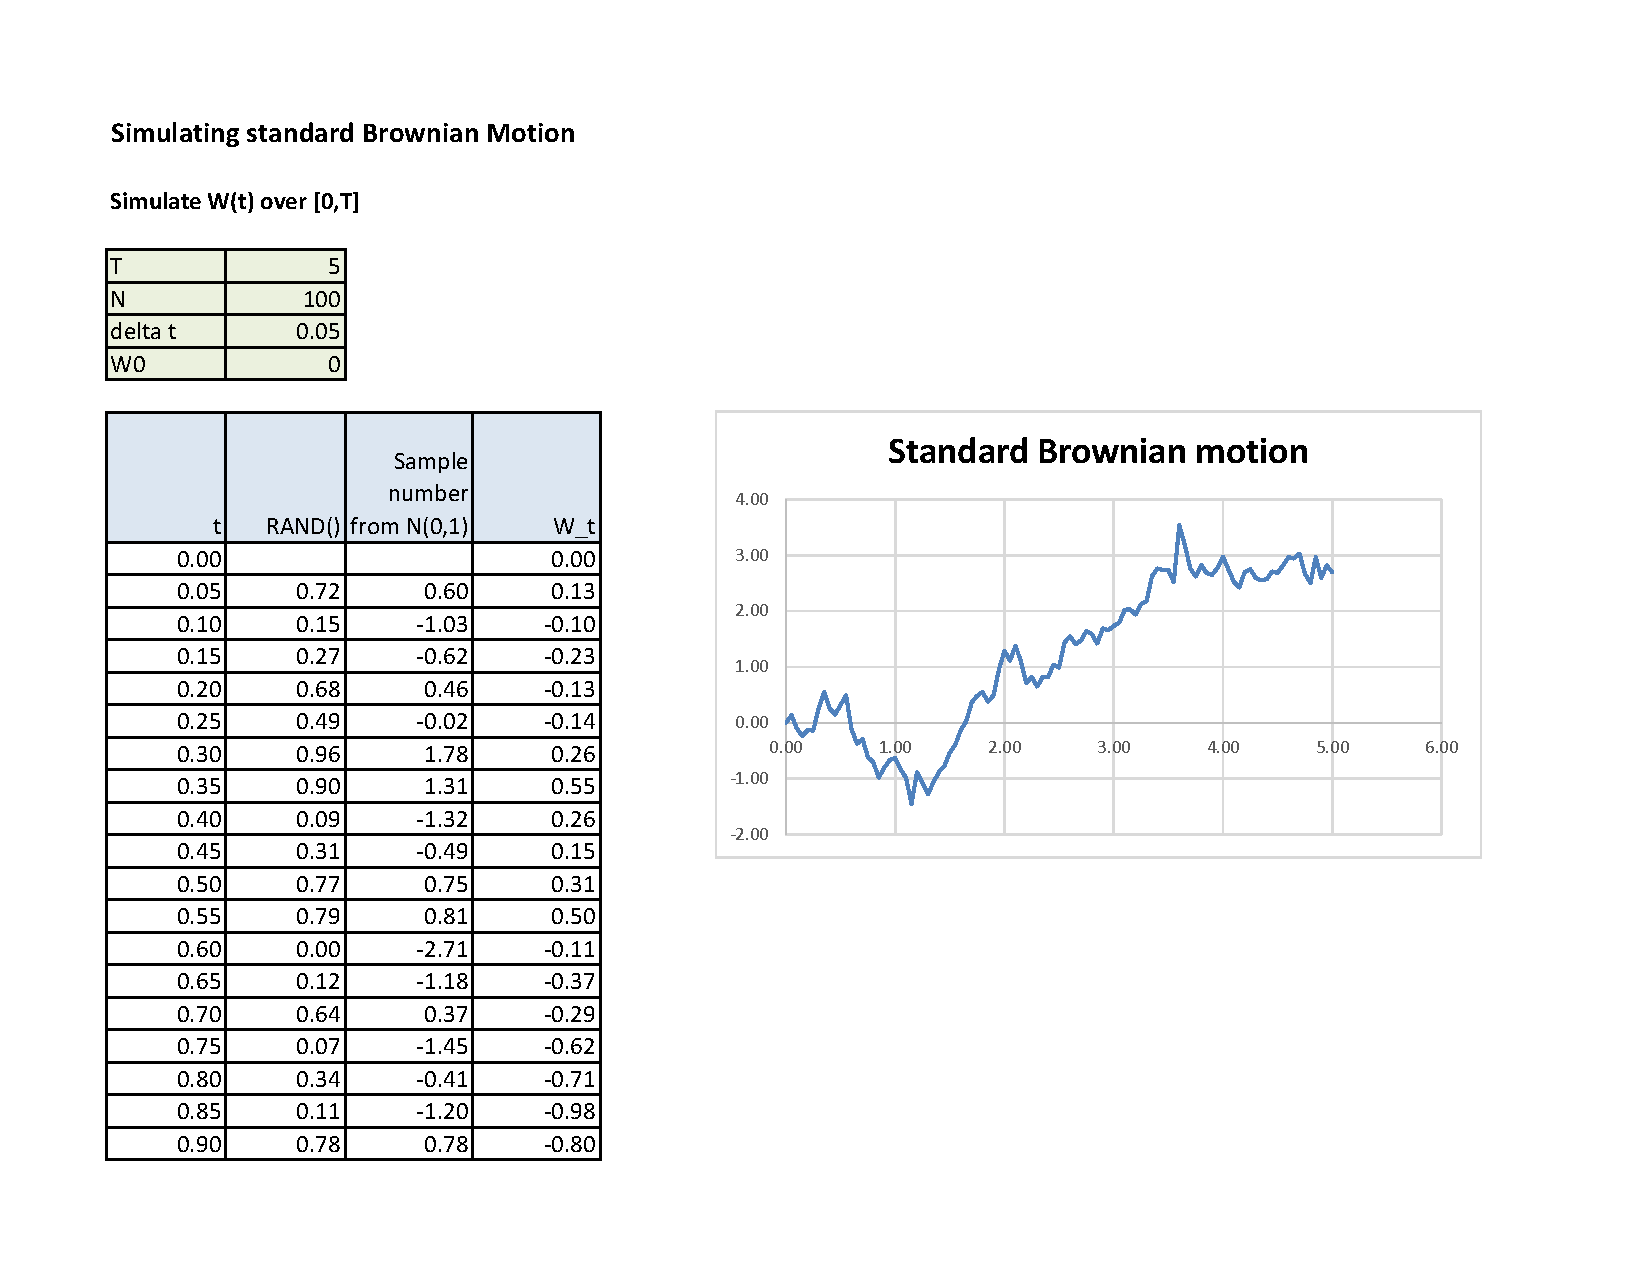
\includegraphics[width=8in,height=\textheight]{BM.pdf}
\caption{Simulating a sample path of the standard Brownian
motion}\label{fig:BM}
}
\end{figure}

In the following example, we do not assume that \(W_0 = 0\) with
probability 1.

\newpage \begin{example}
\protect\hypertarget{exm:unlabeled-div-68}{}\label{exm:unlabeled-div-68}

\emph{Consider a Wiener process denoted by \(W(t)\) with
\(W(0) = a\) with probability 1. The time is measured in years.}

\begin{enumerate}
\def\labelenumi{\arabic{enumi}.}
\item
  \emph{What is the probability distribution of the value of the variable
  at the end of one year, i.e.~\(W(1)\)?}
\item
  \emph{What is the probability distribution of the value of the variable,
  i.e.~\(W(4)\)? and what is the mean and the standard deviation of
  \(W(4)\).}
\end{enumerate}

\emph{What is the probability distribution of the change in the value of W
during 3 months, i.e.~\(W(0.25) - W(0) = W(0.25)\)?}

\end{example}

\hypertarget{generalised-wiener-process-brownian-motion-with-drift}{%
\section{Generalised Wiener process (Brownian Motion with Drift)}\label{generalised-wiener-process-brownian-motion-with-drift}}

In this section, we will consider a variant of the standard Wiener
process, which is modified by introducing the drift and variance
parameters. This new process is known as a \textbf{generalised Wiener
process} or \textbf{Brownian motion with drift}.

More precisely, a generalised Wiener process for a variable \(X\) is
defined in terms of \(dW\) as \[dX = a dt + b dW,\] where \(a\) is a drift
parameter and \(b^2\) is a variance parameter.

\textbf{Note} The process defined above is also known as a \textbf{linear
stochastic differential equation}.

\begin{itemize}
\item
  The term \(a dt\) (deterministic term) implies that \(X\) has an
  \textbf{expected drift rate} of \(a\) per unit of time (or the mean change
  per unit time). To see this, without the stochastic or random
  component \(b dW\), the equation is simply an ordinary differential
  equation \[dX = a dt \quad \text{ or } \quad \frac{dX}{dt} = a.\]
  The solution to this equation with an initial condition \(X(0) = X_0\)
  is \[X = X_0 + a t.\] Clearly, for each time unit the variable \(X\)
  increases by an amount \(a\).
\item
  The stochastic or random component \(b dW\), measured in terms of the
  variance of the change in \(X\), adds \textbf{uncertainty}, \textbf{noise} or
  \textbf{variability} to the path followed by \(X\). The term \(b^2\) is
  referred to as the \textbf{variance rate}.
\end{itemize}

The following example shows that properties of the generalised Wiener
processcan be obtained from the properties of the standard Wiener
process.

\newpage \begin{example}
\protect\hypertarget{exm:unlabeled-div-69}{}\label{exm:unlabeled-div-69}

\emph{Calculate the probability that the generalised Wiener
process \(X(t)\) with the drift parameter \(a = 0.5\) and the variance
\(b^2 = 0.16\) takes the values between 3 and 4 at time \(t = 4\). Assume
that its initial value \(X(0) = 1\).}

\end{example}

\textbf{Solution:} The change of process over 4 units of time is given by
\[X(t) - X(0) = 0.5 \cdot t + 0.4 \cdot (W(t) - W(0)) = 0.5 \cdot t + 0.4 \cdot W(t) .\]
The required probability is \[\begin{aligned}
        \Pr(3 \le X(4) \le 4) &= \Pr( 3 \le  X(0) + 0.5 \cdot 4 + 0.4 \cdot W(4)   \le 4  )\\
            &= \Pr(0 \le W(4) \le 2.5) \\
            &= \Pr(0 \le 2 Z \le 2.5), \text{ where }  Z \sim N(0,1) \\
            &= \Pr(0 \le Z \le 1.25) = 0.3944
    \end{aligned}\] Here we can use the standard normal distribution
table to obtain the probability, or use the Excel function
NORM.S.DIST(z, TRUE), which returns the cumulative distribution of the
standard normal distribution.

\textbf{Notes}

\begin{enumerate}
\def\labelenumi{\arabic{enumi}.}
\item
  The standard Wiener process has the expected drift rate of zero,
  \(a = 0\) and unit variance rate (noise or variability) \(b^2 = 1\). For
  the generalised Wiener process, the amount of this noise or
  variability is \(b\) times a Wiener process. For \textbf{each time unit},
  the Wiener increment \(dW\) follows the standard normal distribution
  \(N(0,1)\). Therefore, the variance per time unit time of the process
  \(X\) is equal to \(b^2\).
\item
  The change in the value of the process \(X\) in any time interval \(t\)
  is normal distributed with mean of \(at\) and variance of \(b^2 t\),
  i.e.~for \(s, t > 0\), \[X(s + t) - X(s) \sim N(at , b^2 t).\] This
  follows from the definition of the process: \[\begin{aligned}
    X(s + t) - X(s)   &= \Delta X  = a \Delta t + b \Delta W\\
                          &= a (s + t  - s) + b  \Delta W = a t + b (W(s + t) - w(s)) \\
                      &\sim at + b \cdot N(0, t) = N(at, b^2 t),\end{aligned}\]
  since \(W(s + t) - w(s) \sim N(0,t)\).
\item
  In general, the drift and variance rates of a stochastic process may
  depend on both \(X\) and \(t\). The process is called an Itô process and
  can be written as \[dX = a(X,t) dt + b(X,t) dW,\] where \(a\) and \(b\)
  are functions of \(X\) and \(t\).
\end{enumerate}

\newpage \begin{example}
\protect\hypertarget{exm:unlabeled-div-70}{}\label{exm:unlabeled-div-70}

\emph{Consider the cash position of a company measured in
millions of Thai baht. Assume that it follows a generalised Wiener
process with a drift of 10 per year and a variance rate of 400 per year.
Let \(X(0) = 50\).}

\begin{enumerate}
\def\labelenumi{\arabic{enumi}.}
\item
  \emph{What is the distribution of the process at the end of the first
  year, \(X(1)\)?}
\item
  \emph{What is the distribution of the process at the end of 6 months,
  \(X(1/2)\)?}
\item
  \emph{What is the probability that the cash position will be at least 60
  million baht at the end of 6 months?}
\end{enumerate}

\end{example}

\textbf{Solution:}

\begin{enumerate}
\def\labelenumi{\arabic{enumi}.}
\item
  At the end of the first year, we know that
  \[X(1) - X(0) \sim N(a \cdot 1, b^2 \cdot 1),\] where \(a = 10\) and
  \(b^2 = 400\). It follows that
  \[X(1) \sim N(X(0) + a , b^2 ) = N(60, 400).\]
\item
  Similarly, at the end of 6 months,
  \[X(1/2) - X(0) \sim N(a \cdot \frac{1}{2}, b^2 \cdot \frac{1}{2}),\]
  or \[X(1/2) \sim N(55,200).\]
\item
  The required probability is \[\begin{aligned}
          \Pr( X(1/2) \ge 60) &= \Pr( Z \ge \frac{60 - 55}{\sqrt{200}}  )\\
          &= \Pr(Z \ge 0.35) \\
          &= 1 - \text{NORM.S.DIST(0.35, TRUE)} \\
          &= 1 - 0.638 = 0.362.
      \end{aligned}\]
\end{enumerate}

\hypertarget{simulating-a-generalised-wiener-process}{%
\subsubsection{Simulating a generalised Wiener process}\label{simulating-a-generalised-wiener-process}}

Simulating a generalised Wiener process over \([0,T]\) is similar to a
standard Wiener process.

\begin{enumerate}
\def\labelenumi{\arabic{enumi}.}
\item
  We first discretise the interval by let \(\Delta t = T/N\) for some
  positive integer \(N\) and \(t_j = j \cdot \Delta t\).
\item
  Denote \(X(t_j)\) by \(X_j\). The value \(X_j\) can be approximated by
  \[X_j = X_{j-1} + a \Delta t + b \Delta W_j,\] where each
  \(\Delta W_j = W(t_j) - W(t_{j-1})\) is an independent random
  variable of the form \(\sqrt{\Delta t} N(0,1)\).
\end{enumerate}

\begin{figure}
\hypertarget{fig:GW}{%
\centering
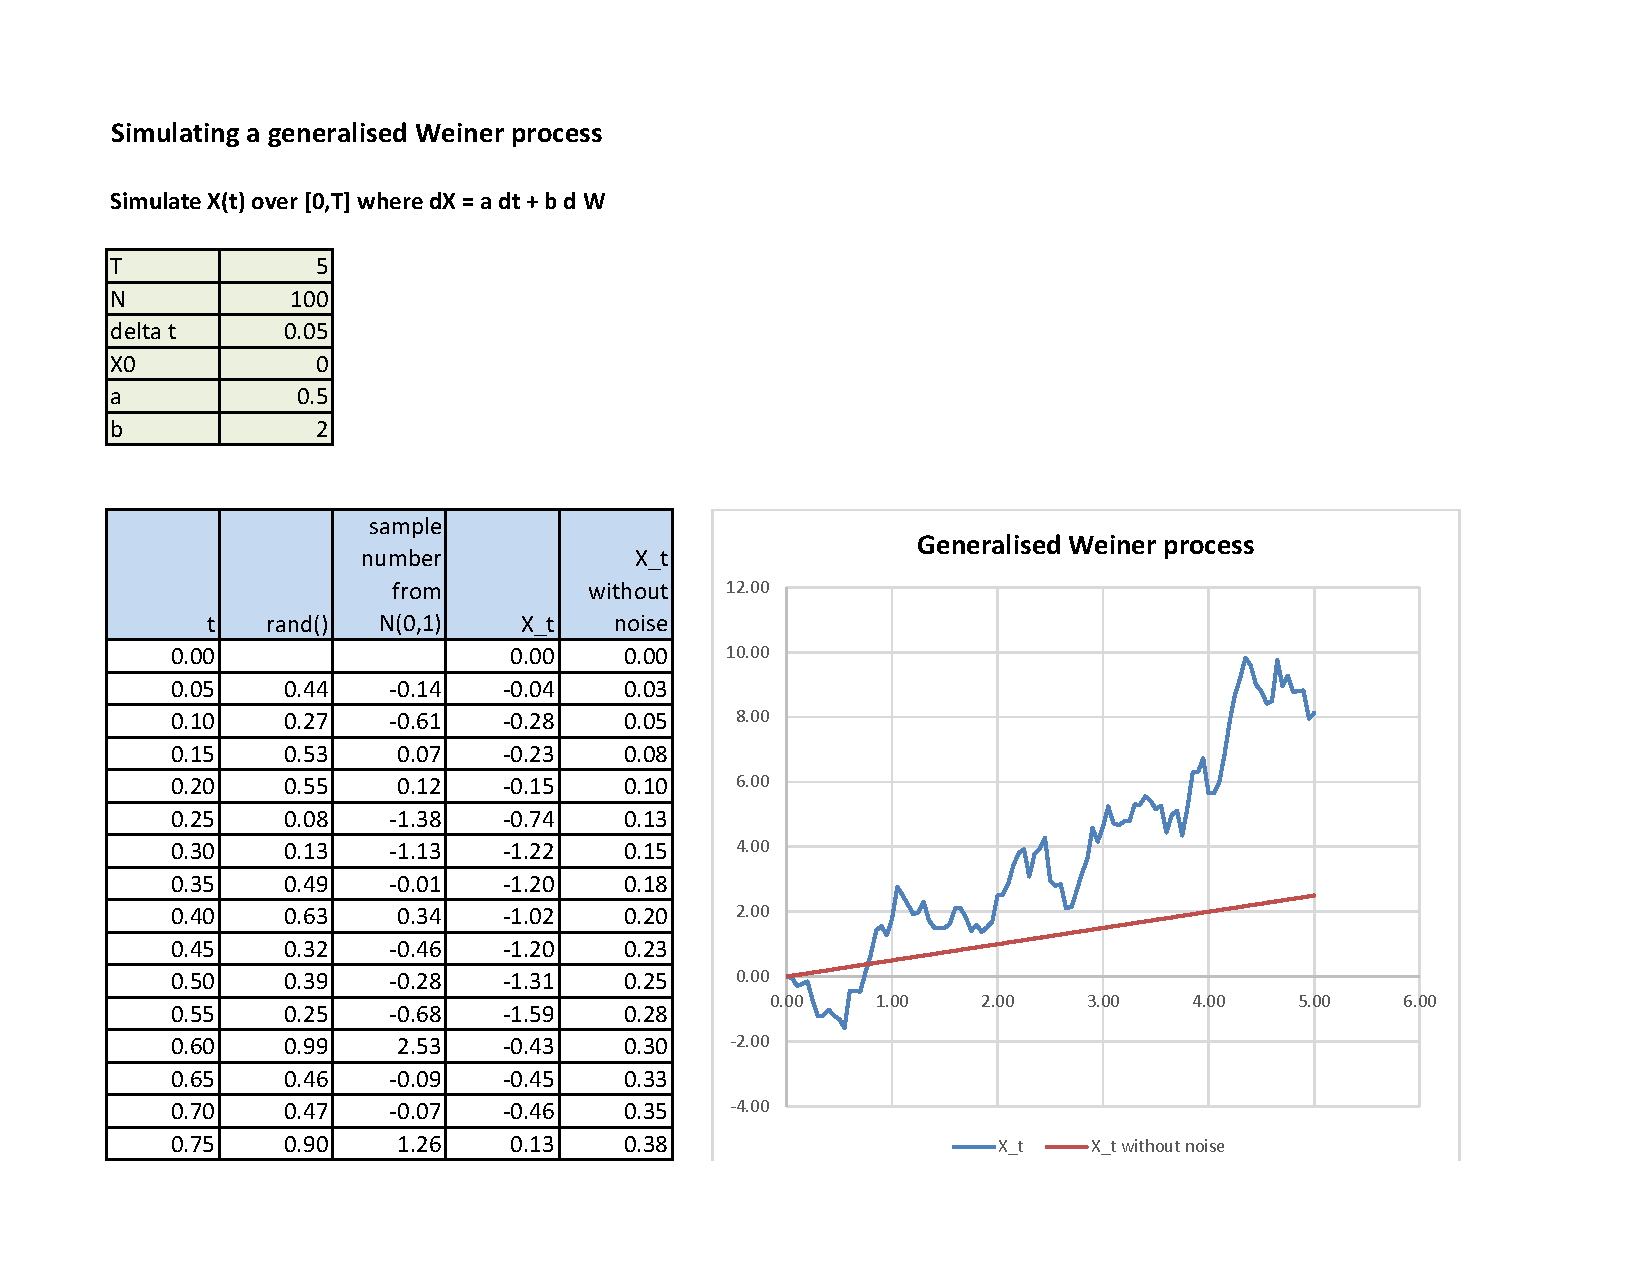
\includegraphics[width=8in,height=\textheight]{GW2.pdf}
\caption{Simulating a sample path of the generalised Wiener process with
\(a =0.5\) and \(b = 2\).}\label{fig:GW}
}
\end{figure}

\textbf{One-Period Simple Return}

Let \(P_t\) be the price of an asset at time index \(t\). Holding the asset
for one period from date t-1 to date t would result in a simple gross
return
\[1 + R_t =  \frac{P_t}{P_{t-1}}   \text{    or     }    P_t = P_{t-1} (1 + R_t).\]

\textbf{Continuously Compounded Return} The natural logarithm of the simple
gross return of an asset is called the continuously compounded return or
log return \[r_t = \ln(1 + R_t) = \ln\frac{P_t}{P_{t-1}}.\]

\hypertarget{the-process-for-a-stock-price}{%
\section{The process for a stock price}\label{the-process-for-a-stock-price}}

We will discuss a simple model (or a stochastic process) for the price
of a non-dividend-paying stock. The model is known as \textbf{geometric
Brownian motion}. We will show that this stochastic model assumes or
implies the following properties for stock prices.

\begin{enumerate}
\def\labelenumi{\arabic{enumi}.}
\item
  The process is \textbf{continuous in time and value}.
\item
  It possesses the \textbf{Markov property}, i.e.~future prices depend only
  on its the current stock price and not on its the past historical
  values.
\item
  The \textbf{proportional return on a stock} over a short time interval is
  normally distributed.
\item
  The \textbf{price of a stock} is lognormally distributed.
\item
  The \textbf{continuously compounded rate of return per year} for a stock
  is normally distributed.
\end{enumerate}

\newpage \begin{example}
\protect\hypertarget{exm:unlabeled-div-71}{}\label{exm:unlabeled-div-71}

\emph{Explain why a generalised Wiener (GW) process is
inappropriate to model a stock price.}

\end{example}

\textbf{Solution:} The GW model assumes that the expected change (not the
return) is independent of the stock price, which does not explain a key
aspect of stock prices. The expected percentage return (not the change
in stock price) required by an investor in a short period of time,
\(\Delta t\), should be the same regardless of the stock price.

In particular, when either the stock price is ฿100 or ฿1000, the
investor would require the same expected return.

\hypertarget{model-assumptions-of-the-geometric-brownian-motion}{%
\subsection{Model Assumptions of the Geometric Brownian Motion}\label{model-assumptions-of-the-geometric-brownian-motion}}

The geometric Brownian motion also consists of two components:

\begin{enumerate}
\def\labelenumi{\arabic{enumi}.}
\item
  \textbf{The deterministic component:} The model assumes that the expected
  drift rate in \(S\) (the mean change in \(S\) per unit of time) is
  proportion to the price \(S\), i.e.~equal to \(\mu S\), for some
  constant parameter \(\mu\). As a result, the expected increase in \(S\)
  in a short time interval \(\Delta t\) is \(\mu S \Delta t\). Therefore,
  without uncertainty, the model can be expressed as
  \[\Delta S = \mu S \Delta t\] As \(\Delta t \rightarrow 0,\) the model
  can be described by an ordinary differential equation
  \[\frac{dS}{dt} = \mu S,\] and the solution to this differential
  equation is \[S_{T} = S_0 \exp(\mu T),\] where \(S_0\) and \(S_T\) are
  the stock prices at time 0 and time \(T\).

  \textbf{Note} When there is no uncertainty, the stock price grows at a
  continuously compounded rate of \(\mu\) per unit of time (generally
  per year). If the price of the stock today is \(S_0\), then its price
  \(S_T\) at time \(T\) is \(S_{T} = S_0 \exp(\mu T)\).
\item
  \textbf{The stochastic component:}

  An additional assumption of the model is that the variability of the
  percentage return (\(\Delta S/S\)) in a short time period \(\Delta t\)
  is the same regardless of the stock price. This means that the
  uncertainty of the percentage return when the stock price is ฿100 is
  the same as that when the stock price is ฿250.

  This assumption adds stochastic or random component into the model.

  As a result, by adding the stochastic or random component to the
  deterministic component, the \textbf{geometric Brownian motion} can be
  expressed as \[dS = \mu S dt + \sigma S dW\] where \(W\) is a standard
  Brownian motion (or a Weiner process).
\end{enumerate}

\textbf{Notes}

\begin{enumerate}
\def\labelenumi{\arabic{enumi}.}
\item
  The geometric Brownian motion is the continuous-time version of a
  random walk.
\item
  The discrete-time version of the geometric Brownian motion is
  \[\frac{\Delta S}{S} = \mu \Delta t + \sigma \sqrt{\Delta t} \epsilon,\]
  where \(\epsilon\) has a standard normal distribution (with zero mean
  and unit variance ) The parameter \(\mu\) is the \textbf{expected rate of
  return per unit of time} from the stock, and \(\sigma\) is the
  \textbf{volatility} of the stock price.
\end{enumerate}

\hypertarget{proportional-return-on-stocks-are-normally-distributed}{%
\subsubsection{Proportional return on stocks are normally distributed}\label{proportional-return-on-stocks-are-normally-distributed}}

It follows from the definition of the the geometric Brownian motion that
the proportional return on the stock over a short time interval is
normally distributed with a mean \(\mu \Delta t\) and variance of
\(\sigma^2 \Delta t\). In particular, \[\begin{aligned}
\label{propReturn}
\frac{\Delta S}{S} = N( \mu \Delta t , \sigma^2  \Delta t).\end{aligned}\]

\newpage \begin{example}
\protect\hypertarget{exm:unlabeled-div-72}{}\label{exm:unlabeled-div-72}

\emph{Consider a stock that pays no dividends, provide an
expected return of 20\% per annum with continuous compounding and has a
volatility of 40\% per annum. Assume that the current stock price is ฿20
and \(\epsilon\) sampled from the standard normal distribution is 0.6.}

\begin{enumerate}
\def\labelenumi{\arabic{enumi}.}
\item
  \emph{Calculate the change of the stock price over 1 day, assuming that
  there are 250 trading days per year.}
\item
  \emph{Calculate the stock price over 10 days if the random samples for
  \(\epsilon\) are given in Figure~\protect\hyperlink{fig:GBM}{3.6}.}
\end{enumerate}

\end{example}

\textbf{Solution:}

\begin{enumerate}
\def\labelenumi{\arabic{enumi}.}
\item
  Given that \(\mu = 0.2\) and \(\sigma = 0.4\) per annum, the process of
  the stock price is \[\frac{dS}{S} = \mu dt + \sigma dW.\] Here \(S\)
  is the stock price at a particular time. If \(\Delta S\) is the change
  in the stock price in the next small interval \(\Delta\)t of time,
  then the discrete-time version of the model is \[\begin{aligned}
      \frac{\Delta S}{S} &= \mu \Delta t + \sigma \sqrt{\Delta t} \epsilon \\
                     &= 0.2 \Delta t + 0.4 \sqrt{\Delta t} \epsilon,
      \end{aligned}\] where \(\epsilon\) has a standard normal
  distribution.

  For a time interval of 1 day or 0.004 years,
  \[\frac{\Delta S}{S} = 0.2 \cdot 0.004 + 0.4 \sqrt{0.004} \epsilon.\]
  If the current stock price is 20 and \(\epsilon = 0.6\), then
  \[\Delta S = 20(0.2 \cdot 0.004 + 0.4 \sqrt{0.004} 0.6) = 0.3196,\]
  and \(S(0.004) = S(0) + \Delta S = 20.3196.\)
\item
  Leave as an exercise.
\end{enumerate}

\begin{figure}
\hypertarget{fig:GBM}{%
\centering
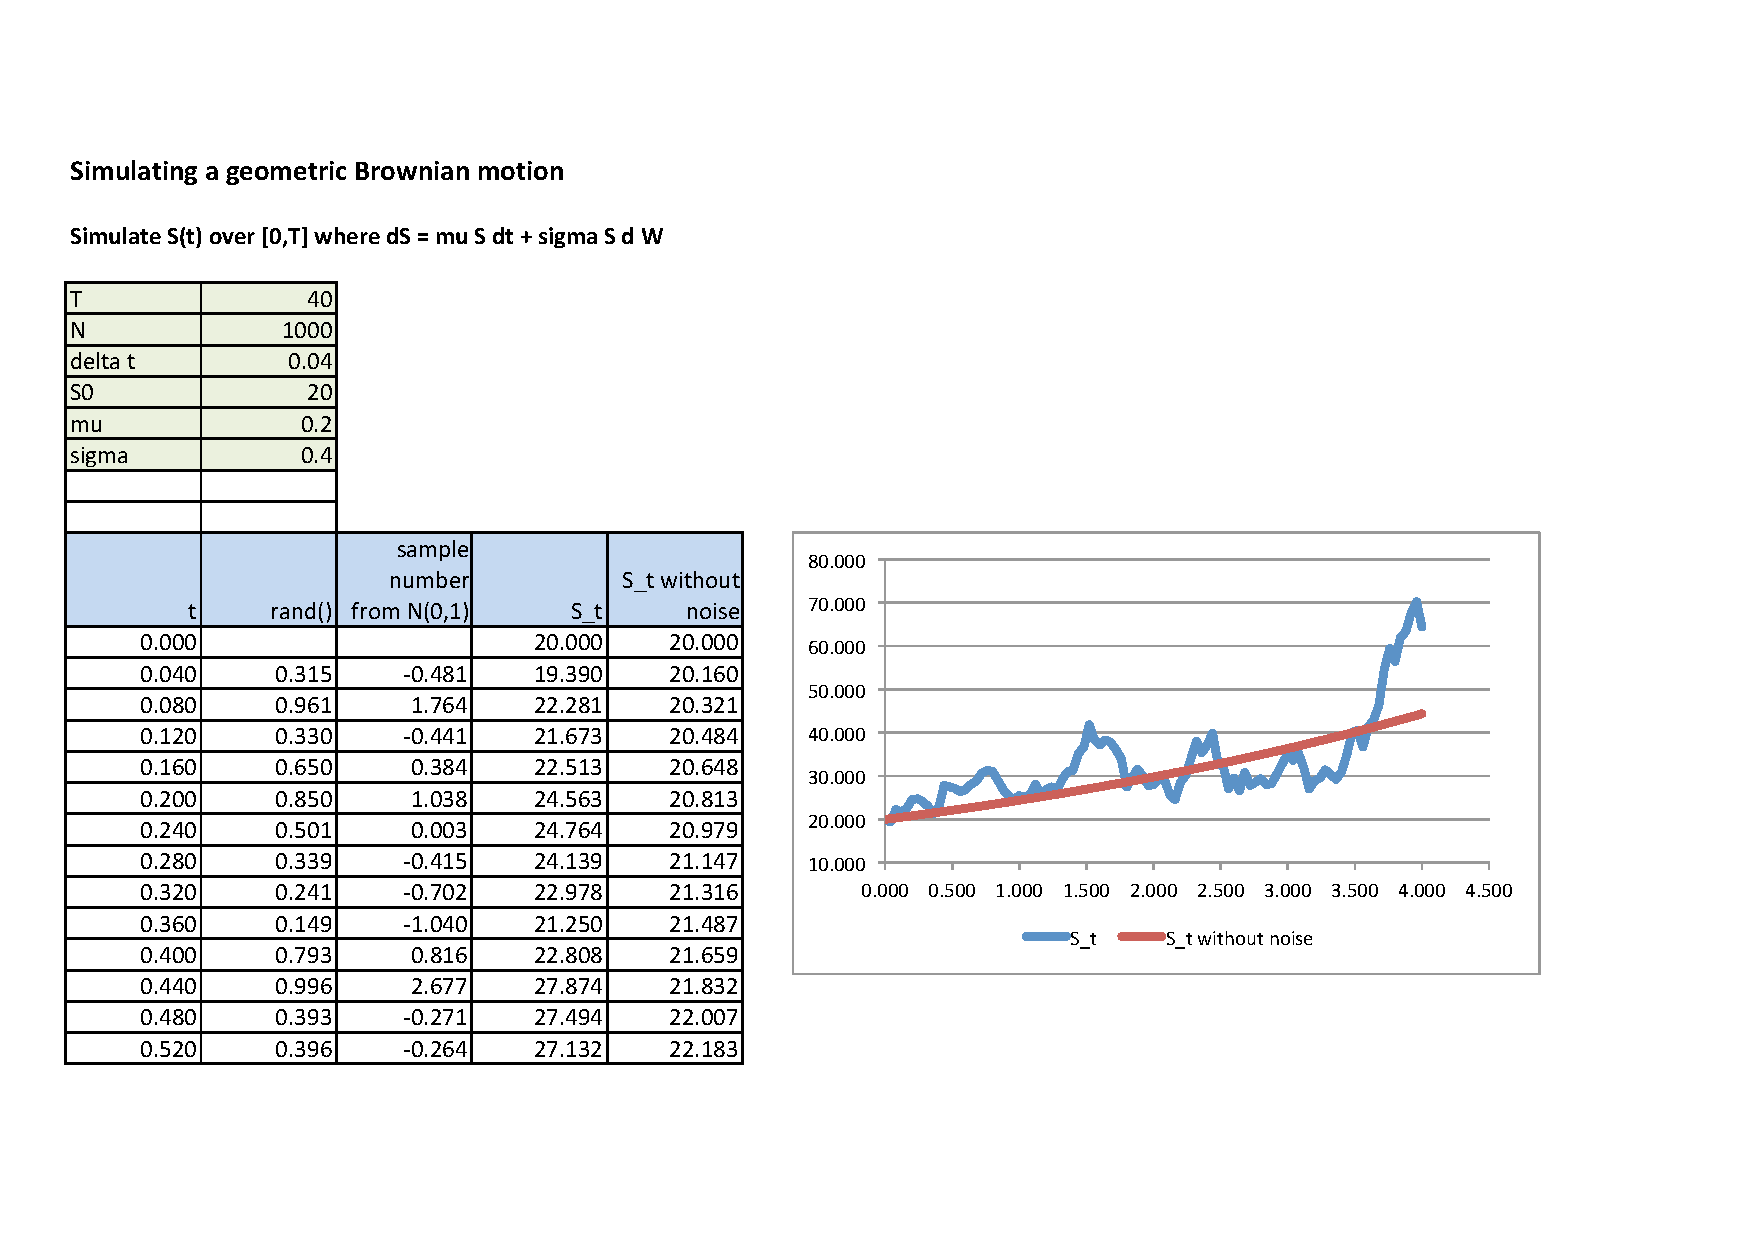
\includegraphics[width=8in,height=\textheight]{GBM.pdf}
\caption{Simulating a sample path of a geometric Brownian motion with
\(\mu =0.2\) and \(\sigma = 0.4\).}\label{fig:GBM}
}
\end{figure}

\textbf{Notes}

\begin{enumerate}
\def\labelenumi{\arabic{enumi}.}
\item
  The parameter \(\mu\) is the annualised expected return in a short
  period of time. It should depend on the risk of the return from the
  stock, and should also depend on the level of interest rates in the
  market. The higher the interest rates, the higher the expected
  return.
\item
  The value of a (financial) derivative, for example options, is
  independent of \(\mu\). So we do not need to concern with the
  estimation of \(\mu\).
\item
  The parameter \(\sigma\), the stock price volatility, is important to
  determine the value of (financial) derivatives. We will discuss how
  to estimate \(\sigma\).
\item
  The standard deviation of the proportional change in the stock price
  in a \textbf{small interval} \(\Delta t\) is \(\sigma \sqrt{\Delta t}\). For
  a \textbf{relatively long period} of time \(T\), it is approximately equal
  to \(\sigma \sqrt{T}\).

  As a result, \textbf{the volatility \(\sigma\) can be interpreted as the
  standard deviation of the change in the stock price in 1 year}.
\end{enumerate}

\hypertarget{stock-prices-are-lognormally-distributed}{%
\subsection*{Stock prices are lognormally distributed}\label{stock-prices-are-lognormally-distributed}}
\addcontentsline{toc}{subsection}{Stock prices are lognormally distributed}

Using Itô lemma (from stochastic calculus), it follows that stock prices
are lognormally distributed: \[\begin{aligned}
 \label{lognormal}
 \ln \frac{S_T}{S_0} \sim N\left((\mu - \frac{\sigma^2}{2})T,\sigma^2 T\right)
 \end{aligned}\] and
\[\ln S_T \sim N\left(\ln S_0 +  (\mu - \frac{\sigma^2}{2})T,\sigma^2 T\right)\]
where \(S_T\) is the stock price at time \(T\) and \(S_0\) is the stock price
at time 0. Here \(\ln S_T\) is normally distributed and hence \(S_T\) has a
lognormal distribution.

\textbf{Note}

\begin{enumerate}
\def\labelenumi{\arabic{enumi}.}
\item
  The logarithm of a price follows a generalised Wiener process with
  drift rate \(\mu - \sigma^2/2\) and variance rate \(\sigma^2\).
\item
  The mean of the distribution for the change in logarithm of price
  over each time unit (i.e.~log return) is not \(\mu\) but
  \(\mu - \sigma^2/2\).
\item
  Why do stock prices follow a lognormal random variable? Let \(X_i\)
  denotes the percentage change in the stock price during day \(i\).
  Then the stock price at day \(n\) satisfies
  \[S_n = S_0 \cdot X_1 \cdots X_n\] or
  \[\ln(S_n) = \ln(S_0) + \ln(X_1) + \cdots + \ln(X_n).\] Suppose that
  the changes in prices on different days are (identical) independent
  random variables. Then the central limit theorem implies that the
  sum of those independent random variables will be a normal random
  variable. Hence, the stock prices are lognormally distributed.
\item
  Recall that if the random variable \(X\) is lognormally distributed,
  then \(Y = \ln(X)\) has a normal distribution:
  \[X \sim \text{Lognormal}(\mu,\sigma^2)  \Longleftrightarrow \ln(X) \sim N(\mu,\sigma^2).\]

  \(\mathrm{E}[X] = e^{\mu + \frac{1}{2}\sigma^2}, \, \mathrm{Var}[X] = e^{2\mu + \sigma^2}\left( e^{\sigma^2 - 1} \right).\)
\end{enumerate}

\newpage \begin{example}
\protect\hypertarget{exm:unlabeled-div-73}{}\label{exm:unlabeled-div-73}

\emph{Consider a stock that pays no dividends, provide an
expected return of 20\% per annum with continuous compounding and has a
volatility of 40\% per annum. Assume that the current stock price is
฿20.}

\begin{enumerate}
\def\labelenumi{\arabic{enumi}.}
\item
  \emph{Find the probability distribution of the logarithm of the stock
  price \(S_T\) in 3 months' time.}
\item
  \emph{Calculate the mean and the standard deviation of \(\ln S_T\) in 3
  months' time.}
\item
  \emph{Find the 95\% confidence interval of \(S_T\) in 3 months' time.}
\end{enumerate}

\end{example}

\textbf{Solution:}

\begin{enumerate}
\def\labelenumi{\arabic{enumi}.}
\item
  Given that \(\mu = 0.2\), \(\sigma = 0.4\) per annum and \(S_0 = 20\), the
  probability distribution of \(\ln S_T\) in 3 months' time (\(T\) = 0.25
  years) is \[\begin{aligned}
      \ln S_T &\sim  N\left(\ln S_0 +  (\mu - \frac{\sigma^2}{2})T,\sigma^2 T\right) \\
          &= N\left(\ln 20 +  (0.2 - \frac{0.4^2}{2}) 0.25,0.4^2 \cdot 0.25\right) = N(3.026,0.04).\end{aligned}\]
\item
  It follows that for \(T\) = 0.25 years,
  \[\mathrm{E}[\ln S_T] = 3.026,   \text{ and    } \text{SD}(\ln S_T) = \sqrt{0.04} = 0.2.\]
\item
  The 95\% CI of \(\ln S_T\) for \(T\) = 0.25 years, is \[\begin{aligned}
      3.026 - 1.96 \cdot 0.2 &< \ln S_T < 3.026 + 1.96 \cdot 0.2 \\
      2.634 &< \ln S_T < 3.418.\end{aligned}\] Hence,
  \[\begin{aligned}
      e^{2.634} &<  S_T < e^{3.418}\\
          13.93 &<  S_T < 30.51.
      \end{aligned}\] There is a 95\% probability that the stock price
  in in 3 months' time will lie between 13.93 and 30.51.
\end{enumerate}

\textbf{Note} It should be noted that \[\begin{aligned}
    \mathrm{E}[S_T] &= S_0 e^{\mu T} = 20 e^{0.2 \cdot 0.25} = 21.025  \\
     &\neq e^{\mathrm{E}[\ln S_T]}  =  20.615.
    \end{aligned}\] In particular,
\(\ln \mathrm{E}[S_T] \neq \mathrm{E}[\ln S_T]\).

\textbf{Notes}

\begin{enumerate}
\def\labelenumi{\arabic{enumi}.}
\item
  A variable that has a lognormal distribution can take any value
  between zero and infinity. It is not symmetrical unlike the normal
  distribution.
\item
  From the properties of the lognormal distribution, the expected
  value of the stock price is given by (exercises)
  \[\mathrm{E}[S_T] = S_0 \exp (\mu T)\] and the variance of \(S_T\) is
  \[\mathrm{Var}[S_T] = S_0^2 \exp(2 \mu T) (\exp(\sigma^2 T) - 1).\]
\end{enumerate}

\newpage \begin{example}
\protect\hypertarget{exm:unlabeled-div-74}{}\label{exm:unlabeled-div-74}

\emph{Consider a stock that pays no dividends, provide an
expected return of 20\% per annum with continuous compounding and has a
volatility of 40\% per annum. Assume that the current stock price is ฿20.
Calculate the mean and the standard deviation of the stock price \(S_T\)
in 1 year.}

\end{example}

\textbf{Solution:} The mean of \(S_1\) is
\[\mathrm{E}[S_1] =  20 \exp (0.2 \cdot 1)  = 24.428.\] and the variance
of \(S_T\) is
\[\mathrm{Var}[S_1] = 20^2 \exp(2 \cdot 0.2 \cdot 1) (\exp(0.4^2 \cdot 1) - 1) = 103.539.\]
and \[\text{SD}(S_1) = \sqrt{ 103.539} = 10.175.\]

\hypertarget{more-accurate-simulation-the-lognormal-model}{%
\subsection{More accurate simulation : the lognormal model}\label{more-accurate-simulation-the-lognormal-model}}

Because \(T\) can be any time interval, we can use the lognormal
distribution of stock prices to simulate the price of a stock at time
\(t + \Delta t\) given its price at time \(t\). This provides accurately
simulated points along a typical path, regardless of the size of
\(\Delta t\).

The following equations can be use to simulate stock price and estimate
volatility: \[\begin{aligned}
 \label{lognormalModel}
\ln\left(  \frac{S_{t+\Delta t}}{S_t} \right) = (\mu - \frac{1}{2}\sigma^2 )\Delta t + \sigma \epsilon \sqrt{\Delta t}\end{aligned}\]
and
\[S_{t+ \Delta t}  = S_t \exp(   (\mu - \frac{1}{2}\sigma^2 )\Delta t + \sigma \epsilon \sqrt{\Delta t}  )\]

\textbf{Note} The above equations follows from the fact that the process
\(\ln S\) satisfies the following stochastic differential equation
\[d \ln S =  (\mu - \frac{1}{2}\sigma^2 ) \, dt + \sigma \, d W.\]

\hypertarget{the-distribution-of-the-rate-of-return}{%
\subsection{The distribution of the rate of return}\label{the-distribution-of-the-rate-of-return}}

The lognormal property of stock prices can be used to show that the
probability distribution of the \textbf{continuously compounded rate of return
per year} for a stock is \textbf{normally distributed}.

Recall that with the continuously compounded rate \(\delta\) of return per
year, the accumulated value at time \(T\) of the stock \(S_0\) at time 0 is
\[S_T = S_0 \exp(\delta T),\] or
\[\delta = \frac{1}{T} \ln \frac{S_T}{S_0}.\] Hence, it follows that
\[\begin{aligned}
\label{returnRate}
     \delta \sim N\left( \mu - \frac{1}{2}\sigma^2 , \frac{\sigma^2}{T} \right).\end{aligned}\]

\textbf{Notes}

\begin{enumerate}
\def\labelenumi{\arabic{enumi}.}
\item
  The standard deviation of \(\delta\) declines as we consider longer
  time intervals. This means that

  \begin{itemize}
  \item
    if we hold a stock for a short time, our actual return may vary
    significantly from the expected return,
  \item
    but the longer we holder a stock, the more likely we are to earn
    a return close to the expect return.
  \end{itemize}
\item
  When \(T = 1\), the standard deviation of the stock return equal
  \(\sigma\). As been seen earlier, the \textbf{volatility of a stock is the
  standard deviation of the distribution of its continuously
  compounded return per year}.
\end{enumerate}

\hypertarget{the-two-expected-returns-this-section-may-be-skipped}{%
\subsection{The two expected returns (this section may be skipped)}\label{the-two-expected-returns-this-section-may-be-skipped}}

As we have seen, there are two different expected returns of stocks,
\(\mu\) and \(\mu - \sigma^2/2\).

\begin{itemize}
\item
  Equation \protect\hyperlink{propReturn}{\[propReturn\]} shows that the expected percentage change
  (or proportional change) in the stock price in a very short period
  of time, \(\Delta t\) is \(\mu \Delta t\).

  Hence, \(\mu\) is the \textbf{expected rate of return per year for the stock
  for infinitesimal interval of time}.
\item
  Whereas, \(\mu - \sigma^2/2\) is the \textbf{expected continuously
  compounded rate of return per year for finite intervals of time}
  (like days or years), i.e.~realised over a period of time of length
  \(T\) (as shown in Equation
  \protect\hyperlink{returnRate}{\[returnRate\]}).
\end{itemize}

\textbf{Notes}

\begin{enumerate}
\def\labelenumi{\arabic{enumi}.}
\item
  Recall that the expected price of a stock grows at the continuously
  compounded rate of \(\mu\) and we can write
  \[\mathrm{E}[S_T] = S_0 \exp(\mu T).\]
\item
  However, the expected continuously compounded rate of return per
  year for a stock is \(\mu - \sigma^2/2\). This is not the same as the
  rate of return we would calculate from the expected future price of
  stock return. \(\mu\) is not the expected continuously compounded
  return on the stock.
\item
  As a result, we cannot get the expected future price of the stock by
  growing its current price at the expected continuously compounded
  rate of return per year.
\item
  If two stocks have the same price today and the same \(\mu\), then
  their expected prices at any time in the future will be the same.
  The stock with the higher volatility will have a lower continuously
  compounded expected rate of return.
\end{enumerate}

\hypertarget{estimating-volatility}{%
\subsection{Estimating volatility}\label{estimating-volatility}}

There are many different methods to estimate the volatility of a stock.
Here the method is based on a stock's historical volatility calculated
from its daily prices for a certain number of days. As we have seen, the
simulations of a stock price can be simulated by using the following
equation
\[\ln\left(  \frac{S_{t+\Delta t}}{S_t} \right) = (\mu - \frac{1}{2}\sigma^2 )\Delta t + \sigma \epsilon \sqrt{\Delta t}.\]
The estimation of the volatility of the stock price can be done as
follows: Let \(n+1\) denote the number of observations and \(\tau\) to be
the length of observation time interval in years.

\begin{enumerate}
\def\labelenumi{\arabic{enumi}.}
\item
  Given the stock price \(S_i\) at end of the \(i\)th interval for
  \(i = 0,1, \ldots, n\), we define
  \[u_i = \ln \left(\frac{S_i}{S_{i-1}} \right), \quad \text{ for } i = 0,1, \ldots, n\]
\item
  The estimates of the mean and standard deviation of the \textbf{daily
  returns} are given by \[\begin{aligned}
      \bar{u} &= \frac{1}{n} \sum_{i=1}^n u_i \\
      s &= \sqrt{\frac{1}{n-1} \sum_{i=1}^n (u_i - \bar{u})^2 } \\
          &= \sqrt{\frac{1}{n-1} \sum_{i=1}^n    u_i^2 - \frac{1}{n(n-1)}  \left(\sum_{i=1}^n u_i  \right)^2 }\end{aligned}\]
\item
  Because we are using observations at intervals of \(\tau\) measured in
  years, the estimate of the \textbf{annualised volatility} is given by
  \[\hat{\sigma} = \frac{s}{\sqrt{\tau}}.\] The \textbf{standard error of
  this estimate} is approximately \(\hat{\sigma}/\sqrt{2n}\).

  For example, if we use daily prices and assume that there are 250
  trading days in a year, then the time interval is 1/250 years. To
  annualise the daily volatility, we have to multiply \(s\) by
  \(\sqrt{250}\).
\end{enumerate}

\textbf{Note} It follows from
\protect\hyperlink{returnRate}{\[returnRate\]} that the estimated expected return \(\hat{\mu}\)
is given by
\[\hat{\mu}  =  \frac{\bar{u}}{\tau}  + \frac{\hat{\sigma}^2}{2} = \frac{\bar{u}}{\tau}  + \frac{s^2}{2\tau} .\]

\newpage \begin{example}
\protect\hypertarget{exm:unlabeled-div-75}{}\label{exm:unlabeled-div-75}

\emph{Verify the calculation using the stock price
historical data from the table below.}

\end{example}

\textbf{Solution:} See an accompanied Excel file.

\begin{figure}
\hypertarget{fig:volatility}{%
\centering
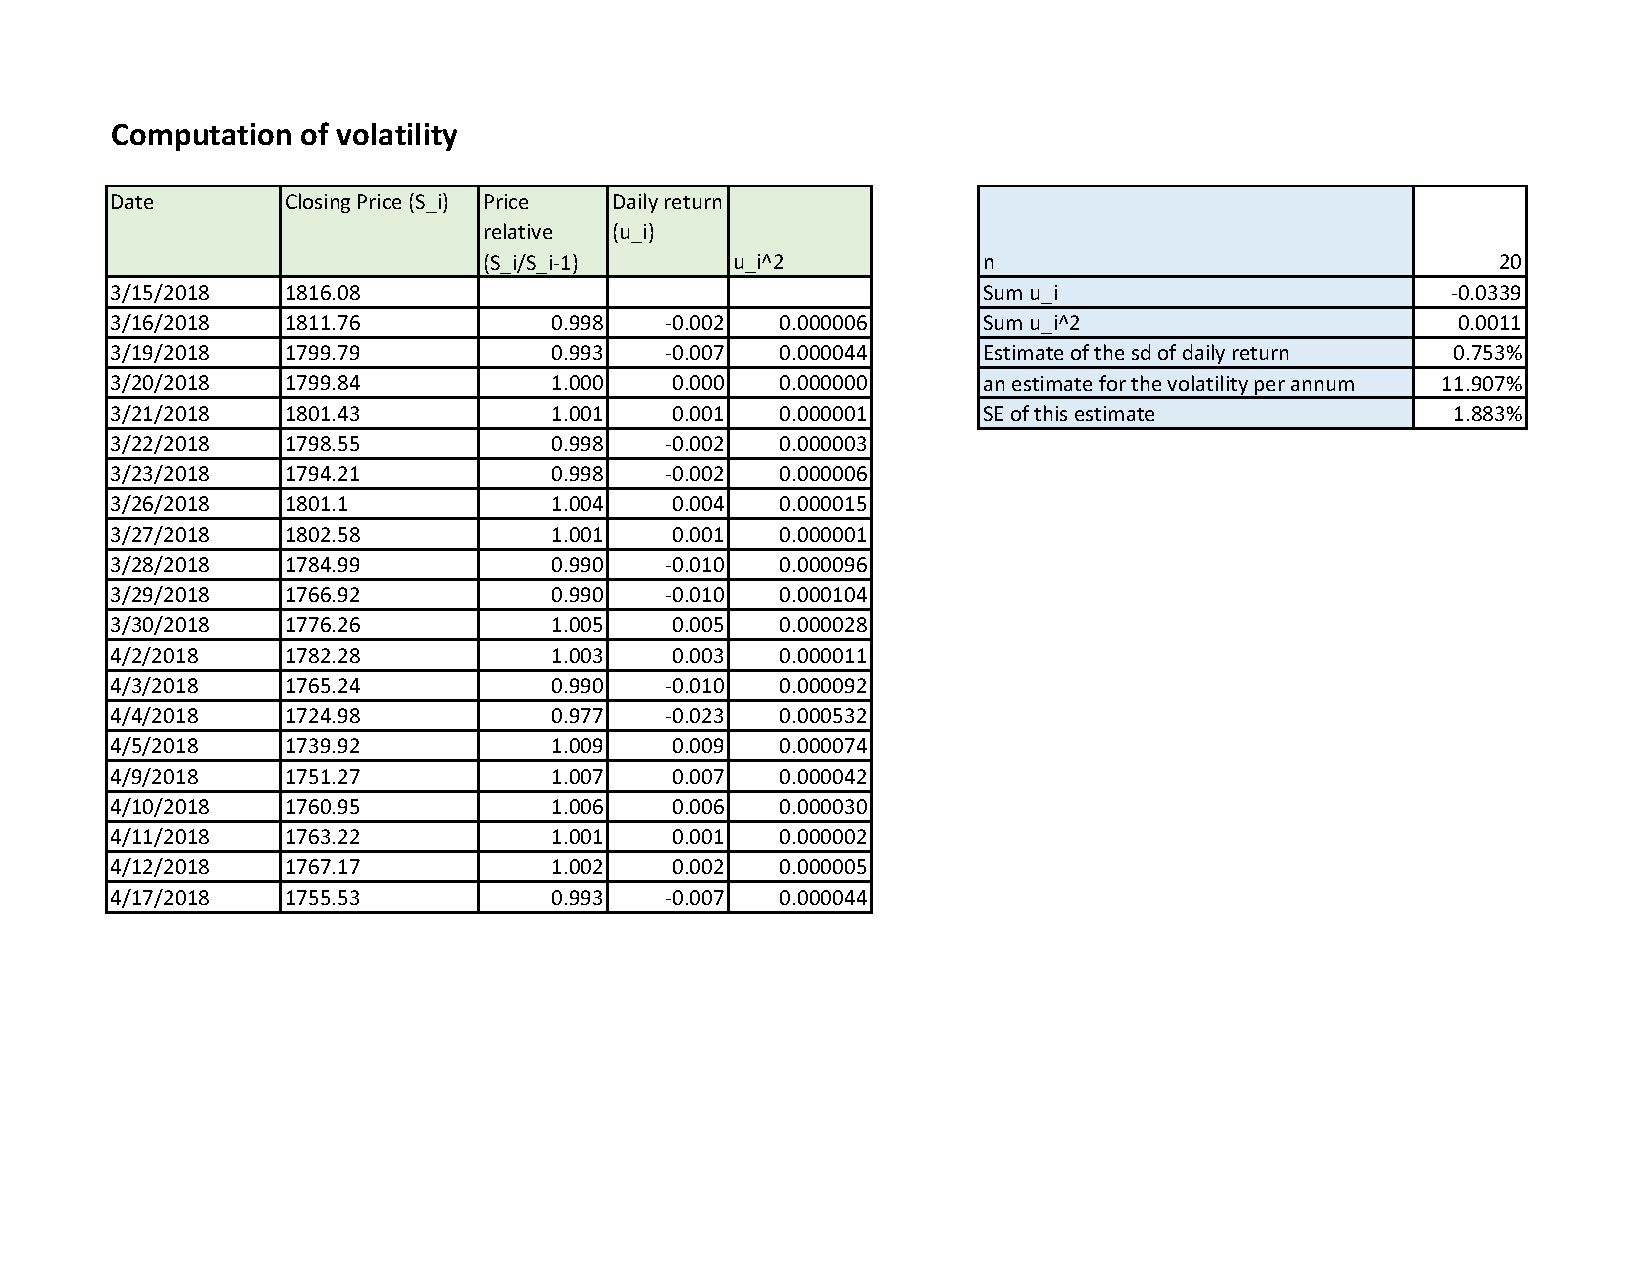
\includegraphics[width=7in,height=\textheight]{VolatilityEstimation2.pdf}
\caption{Computation of volatility}\label{fig:volatility}
}
\end{figure}

\hypertarget{chapter-two}{%
\section{Chapter TWO}\label{chapter-two}}

\hypertarget{chapter-three}{%
\chapter{Chapter THREE}\label{chapter-three}}

\hypertarget{applications}{%
\chapter{Applications}\label{applications}}

Some \emph{significant} applications are demonstrated in this chapter.

\hypertarget{datacamp-light}{%
\section{DataCamp Light}\label{datacamp-light}}

By default, \texttt{tutorial} will convert all R chunks.

eyJsYW5ndWFnZSI6InIiLCJzYW1wbGUiOiJhIDwtIDJcbmIgPC0gM1xuYSArIGIifQ==

  \bibliography{book.bib,packages.bib}

\end{document}
